%-------------------------------------------------------------------------------
% This file provides a skeleton ATLAS note.
% \pdfinclusioncopyfonts=1
% This command may be needed in order to get \ell in PDF plots to appear. Found in
% https://tex.stackexchange.com/questions/322010/pdflatex-glyph-undefined-symbols-disappear-from-included-pdf
%-------------------------------------------------------------------------------
% Specify where ATLAS LaTeX style files can be found.
\newcommand*{\ATLASLATEXPATH}{latex/}
% Use this variant if the files are in a central location, e.g. $HOME/texmf.
% \newcommand*{\ATLASLATEXPATH}{}
%-------------------------------------------------------------------------------
\documentclass[NOTE, atlasdraft=true, texlive=2016, UKenglish]{\ATLASLATEXPATH atlasdoc}
% The language of the document must be set: usually UKenglish or USenglish.
% british and american also work!
% Commonly used options:
%  atlasdraft=true|false This document is an ATLAS draft.
%  texlive=YYYY          Specify TeX Live version (2016 is default).
%  coverpage             Create ATLAS draft cover page for collaboration circulation.
%                        See atlas-draft-cover.tex for a list of variables that should be defined.
%  cernpreprint          Create front page for a CERN preprint.
%                        See atlas-preprint-cover.tex for a list of variables that should be defined.
%  NOTE                  The document is an ATLAS note (draft).
%  PAPER                 The document is an ATLAS paper (draft).
%  CONF                  The document is a CONF note (draft).
%  PUB                   The document is a PUB note (draft).
%  BOOK                  The document is of book form, like an LOI or TDR (draft)
%  txfonts=true|false    Use txfonts rather than the default newtx
%  paper=a4|letter       Set paper size to A4 (default) or letter.

%-------------------------------------------------------------------------------
% Extra packages:
\usepackage{\ATLASLATEXPATH atlaspackage}
% Commonly used options:
%  biblatex=true|false   Use biblatex (default) or bibtex for the bibliography.
%  backend=bibtex        Use the bibtex backend rather than biber.
%  subfigure|subfig|subcaption  to use one of these packages for figures in figures.
%  minimal               Minimal set of packages.
%  default               Standard set of packages.
%  full                  Full set of packages.
%-------------------------------------------------------------------------------
% Style file with biblatex options for ATLAS documents.
\usepackage{\ATLASLATEXPATH atlasbiblatex}

% Package for creating list of authors and contributors to the analysis.
\usepackage{\ATLASLATEXPATH atlascontribute}

% Useful macros
\usepackage{\ATLASLATEXPATH atlasphysics}
% See doc/atlas_physics.pdf for a list of the defined symbols.
% Default options are:
%   true:  journal, misc, particle, unit, xref
%   false: BSM, heppparticle, hepprocess, hion, jetetmiss, math, process, other, texmf
% See the package for details on the options.

% Files with references for use with biblatex.
% Note that biber gives an error if it finds empty bib files.
% \addbibresource{ANA-HDBS-2019-04-INT1.bib}
\addbibresource{bib/ATLAS.bib}
\addbibresource{bib/CMS.bib}
\addbibresource{bib/ConfNotes.bib}
\addbibresource{bib/PubNotes.bib}

% Paths for figures - do not forget the / at the end of the directory name.
\graphicspath{{logos/}{figures/}}

% Add you own definitions here (file ANA-HDBS-2019-04-INT1-defs.sty).
\usepackage{ANA-HDBS-2019-04-INT1-defs}

%-------------------------------------------------------------------------------
% Generic document information
%-------------------------------------------------------------------------------

% Title, abstract and document
%-------------------------------------------------------------------------------
% This file contains the title, author and abstract.
% It also contains all relevant document numbers used for an ATLAS note.
%-------------------------------------------------------------------------------

% Title
\AtlasTitle{DiHiggs HH multilepton full Run2}

% Draft version:
% Should be 1.0 for the first circulation, and 2.0 for the second circulation.
% If given, adds draft version on front page, a 'DRAFT' box on top of each other page, 
% and line numbers.
% Comment or remove in final version.
\AtlasVersion{0.1}

% Abstract - % directly after { is important for correct indentation
\AtlasAbstract{%
  This is a bare bones ATLAS document. Put the abstract for the document here.
}

% Author - this does not work with revtex (add it after \begin{document})
\author{The ATLAS Collaboration}

\AtlasAuthorContributor{Merve Nazlim Agaras}{d}{Int. note editor. Group framework developer and coordinator. Fit contact.}
\AtlasAuthorContributor{Xiaohu Sun}{a}{HH -> yy + 2L: MC signal, statistical analysis}
\AtlasAuthorContributor{Abdualazem Fadol}{b}{HH--> yy + 1/2L, HH -->2LSS, object/event selection, software framework}
\AtlasAuthorContributor{Yaquan Fang}{b}{Analysis contact. HH--> yy + 1/2L, HH -->2LSS, object/event selection, software framework}
\AtlasAuthorContributor{Kaili Zhang}{b}{Combination liason. HH--> yy + 1/2L, HH -->2LSS, object/event selection, software framework}
\AtlasAuthorContributor{Djamel Eddine Boumediene}{d}{QMisID DD estimates. Supervisor of Merve Nazlim Agaras.}
\AtlasAuthorContributor{Maosen Zhou}{b}{HH--> yy + 1/2L, HH -->2LSS, object/event selection, software framework}
\AtlasAuthorContributor{Weiming Yao}{c}{HH -> 1L + jets / 2had taus + jets: Tau selection and fakes}
\AtlasAuthorContributor{Rohin Narayan}{e}{HH -> 2L/3L: Fake leptons, kinematic discriminants, software framework} 
\AtlasAuthorContributor{Allison McCarn Deiana}{e}{HH -> 2L/3L: Fake leptons, kinematic discriminants, software framework}
\AtlasAuthorContributor{Xingguo Li}{f}{HH -> 2/3L + jets}
\AtlasAuthorContributor{Chihao Li}{g}{HH -> 4L + 2b: MC generation, object definition, event selection, combination}
\AtlasAuthorContributor{Yusheng Wu}{g}{HH -> 4L + 2b: MC generation, object definition, event selection, combination}
\AtlasAuthorContributor{Bartlomiej Zabinski}{h}{HH -> taus + X: Tau optimisation, machine learning, fit, framework}
\AtlasAuthorContributor{Anna Kaczmarska}{h}{HH -> taus + X: Tau optimisation, machine learning, fit, framework}
%\AtlasAuthorContributor{Ana Elena Dumitriu}{j, i}{Support in group framework 1.} Tiesheng Dai, Hang Qi, Bing Li, Bing Zhou
\AtlasAuthorContributor{Tiesheng Dai}{i}{HH -> 4L + 2b: MC signal, object definition, event selection, interpretation, combination}
\AtlasAuthorContributor{Hang Qi}{i}{HH -> 4L + 2b: MC signal, object definition, event selection, interpretation, combination}
\AtlasAuthorContributor{Bing Zhou}{i}{HH -> 4L + 2b: MC signal, object definition, event selection, interpretation, combination}
\AtlasAuthorContributor{Huirun Chen}{j}{HH->1L+3tau had: MC signal production, truth studies}
\AtlasAuthorContributor{Xiaozhong Huang}{j}{HH->1L+3tau had: MC signal production, truth studies}
\AtlasAuthorContributor{Bowen Zhang}{j}{HH->1L+3tau had: MC signal production, truth studies}
\AtlasAuthorContributor{Lei Zhang}{j}{HH->1L+3tau had: MC signal production, truth studies}
\AtlasAuthorContributor{Liang Li}{k}{HH -> 2/3L + jets}
\AtlasAuthorContributor{Jiannan Tang}{k}{HH -> 2/3L + jets}
\AtlasAuthorContributor{Lebohang Mokoena}{l}{X -> SH -> 2L + jets: MC signal, event selection, bkg estimation, statistical analysis}
\AtlasAuthorContributor{Bruce Mellado}{l}{X -> SH -> 2L + jets: MC signal, event selection, bkg estimation, statistical analysis}
\AtlasAuthorContributor{Lehumo Mashishi}{l}{X -> SH -> 2L + jets: MC signal, event selection, bkg estimation, statistical analysis}
\AtlasAuthorContributor{Jeremiah Kgomotso Monnakgotla}{l}{X -> SH -> 2L + jets: MC signal, event selection, bkg estimation, statistical analysis}
%\AtlasAuthorContributor{Dylan Kisliuk}{f}{Tau fake estimates.}
\AtlasAuthorContributor{Yesenia Hernandez}{l}{Analysis contact. X -> SH -> 2L + jets: MC signal, event selection, bkg estimation, statistical analysis}

\affil[a]{Manchester}
\affil[b]{Beijing IHEP	}
\affil[c]{Berkeley LBNL	}
\affil[d]{LPC Clermont-Ferrand}
\affil[e]{Dallas SMU}
\affil[f]{DESY}
\affil[g]{USTC}
\affil[h]{Krakow IFJ PAN}
\affil[i]{Michigan}
\affil[j]{Nanjing}
\affil[k]{Shanghai}
\affil[l]{Witwatersrand}






% Authors and list of contributors to the analysis
% \AtlasAuthorContributor also adds the name to the author list
% Include package latex/atlascontribute to use this
% Use authblk package if there are multiple authors, which is included by latex/atlascontribute
% \usepackage{authblk}
% Use the following 3 lines to have all institutes on one line
% \makeatletter
% \renewcommand\AB@affilsepx{, \protect\Affilfont}
% \makeatother
% \renewcommand\Authands{, } % avoid ``. and'' for last author
% \renewcommand\Affilfont{\itshape\small} % affiliation formatting
% \AtlasAuthorContributor{First AtlasAuthorContributor}{a}{Author's contribution.}
% \AtlasAuthorContributor{Second AtlasAuthorContributor}{b}{Author's contribution.}
% \AtlasAuthorContributor{Third AtlasAuthorContributor}{a}{Author's contribution.}
% \AtlasContributor{Fourth AtlasContributor}{Contribution to the analysis.}
% \author[a]{First Author}
% \author[a]{Second Author}
% \author[b]{Third Author}
% \affil[a]{One Institution}
% \affil[b]{Another Institution}


% If a special author list should be indicated via a link use the following code:
% Include the two lines below if you do not use atlasstyle:
% \usepackage[marginal,hang]{footmisc}
% \setlength{\footnotemargin}{0.5em}
% Use the following lines in all cases:
% \usepackage{authblk}
% \author{The ATLAS Collaboration%
% \thanks{The full author list can be found at:\newline
%   \url{https://atlas.web.cern.ch/Atlas/PUBNOTES/ATL-PHYS-PUB-2016-007/authorlist.pdf}}
% }

% ATLAS reference code, to help ATLAS members to locate the paper
\AtlasRefCode{ANA-HDBS-2019-04}

% ATLAS note number. Can be an COM, INT, PUB or CONF note
\AtlasNote{ANA-HDBS-2019-04-INT1}

% Author and title for the PDF file
\hypersetup{pdftitle={ATLAS document},pdfauthor={The ATLAS Collaboration}}
\usepackage{multirow}

%-------------------------------------------------------------------------------
% Content
%-------------------------------------------------------------------------------
\begin{document}

\maketitle

\tableofcontents

% List of contributors - print here or after the Bibliography.
\PrintAtlasContribute{0.30}
%\clearpage

% Tex for mainbody
\clearpage
%\input{Tex/Status.tex}
\clearpage
\section{Introduction}
\label{sec:intro}

With the discovery of a new scalar particle the Higgs boson~\cite{HIGG-2012-27,CMS-HIG-12-028} at the LHC~\cite{Evans:2008zzb} by the ATLAS and CMS collaborations with a mass of 125 GeV~\cite{HIGG-2016-33,HIGG-2013-12,HIGG-2014-14,CMS-HIG-14-009}, the whole content of the Standard Model (SM) of particle physics became complete. A priority of the ATLAS and CMS collaborations has been to better understand its properties and couplings.
After the EWSB and the higgs field acquires the vev, the higgs potential obtained in Equation.. can be obtained as following:
\begin{align}
	V(\phi) \rightarrow V(\phi)_{\text{EWSB}} =  -\lambda \nu^2 h^2 - \lambda \nu h^3 - \frac{1}{4} \lambda h^4 + \text{const.}
	\label{eq:higgs_pot}
\end{align}
The first term of the above equation is the Higgs mass term, and the remaining are the trilinear and quadri-linear Higgs-self couplings,
\begin{align}
	\underbrace{m_{h} = \sqrt{ - 2 \mu^2} = \sqrt{ 2 \lambda v^2 }}_\text{Higgs boson mass} \hspace{1cm} \underbrace{\lambda_{hhh} \propto \frac{m_h^2}{v} \hspace{1cm} \lambda_{hhhh} \propto \frac{m_h^2}{v^2}}_\text{Trilinear and quadri-linear Higgs self-couplings}.
	\label{eq:higgs_self_couplings}
\end{align}
A measurements of this couplings would therefore give a hint about the actual structure of the potential, whose shape can have  theoretical consequences. The quartic Higgs coupling, $\lambda_{hhhh}$, can not be measured at LHC since the cross-section of triple Higgs production is small~\cite{PhysRevD.74.113008}~\cite{PhysRevD.93.035026}, while the trilinear coupling can be probed directly in Higgs pair production. 

The trilinear coupling leads to non-resonant pair production of Higgs bosons, where an off-shell
Higgs decays to a pair of Higgs bosons, the leading production mechanism being $gg$-fusion.
Direct observation of Higgs pair production would lead to measurements directly sensitive to
$\lambda$ but in the SM there are competing diagrams, proceeding via quark (re: top quark) loops
that are instead senstive to the Yukawa coupling of the Higgs rather than the trilinear coupling
$\lambda$. These \dihiggs production mechanisms are illustrated in the Feynman diagrams presented
in Figure \ref{fig:sm_nonres_hh}. Not only does the quark-loop induced process present
itself as an irreducible background to the process senstive to the Higgs self-coupling, but
it interfereces \textit{destructively} with the latter, making the observation of this
type of Higgs pair production more challenging.


% Due to its lower cross section, diHiggs production is not expected to be observed in the current data taking setup, however it is possible to define limits on the measurement to constrain the BSM physics theories. 
\begin{figure}[!htb]
    \centering
    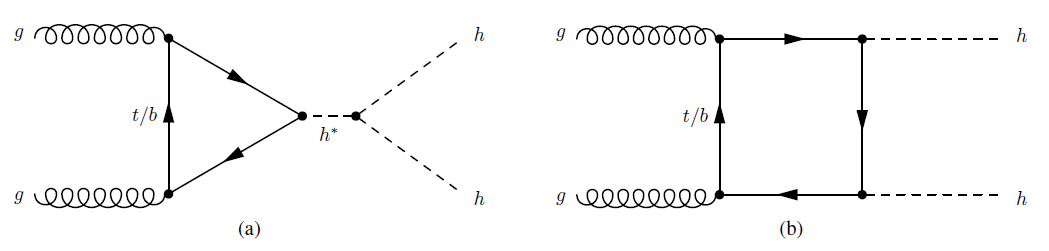
\includegraphics[width=0.9\textwidth]{figures/sm_nonres_hh_production}
    \caption{Representative diagrams that contribute to non-resonant \hh production.
    \textit{Left}: Diagram that is sensitive to the trilinear coupling, $\lambda$.
    \textit{Right}: Box diagram that interferese destructively with the $\lambda$-sensitive
    process.} 
    \label{fig:sm_nonres_hh}
\end{figure}


As a result of the destructive interference, and the already relatively large Higgs mass of
125 \GeV, the SM \dihiggs production has a total cross-section of $\sim 33.4$ fb ~\cite{CERN-YR-4}
at a \pp center-of-mass collision energy of 13 \TeV. The inclusive cross-section for the pair-production
of top quarks, which will be one of the dominant SM backgrounds in the present
analysis, is nearly 1000 pb, or $1\times10^6$ fb ~\cite{TOPQ-2015-09, ATLAS-CONF-2015-049}. That
of \textit{single} Higgs production is $\sim 50$ pb, or $5 \times 10^4$ fb ~\cite{ATLAS-CONF-2015-060}.

Furthermore, enhancements to the di-Higgs production rate, either non-resonantly or through a resonance, may be observable with the full Run2 dataset and would point to new physics beyond the Standard Model, making such analyses interesting now. The wide class of two Higgs double models (2HDM) predict an altered and enlarged
Higgs sector from which the currently Higgs is built.
The Minimal Supersymmetric Standard Model
(MSSM) is a  class of 2HDM. For the latter set, one such model is a Randall-Sundrum
type graviton or the lightest Kaluza-Klein excitation which have masses of at least
$2\times$ the mass of the SM Higgs boson. The presence of such BSM scenarios would act to alter
the measured value of $\lambda$ with respect to that of the SM, potentially enlarging it.
As a result, early evidence for the pair-production of Higgs bosons within the current
Run-2 dataset may indicate the presence of new physics without having to resort to
precision measurements of $\lambda$. Examples of such decay
scenarios are illustrated in example Feynman diagrams in Figure \ref{fig:2hdm_feynman_diagrams}.

\begin{figure}[!htb]
    \centering
    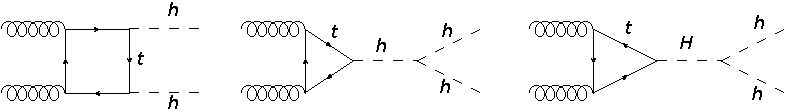
\includegraphics[width=0.8\textwidth]{figures/mg5_hh_heavy_scalar.png}
    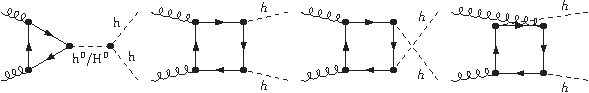
\includegraphics[width=0.8\textwidth]{figures/mg5_hh_2hdm_cp_even.png}
    \caption
    {
        Diagrams contributing to enhanced $hh$ production scenarios.
        \textit{Top}: A heavy scalar, $H$, that couples to the Standard Model Higgs
        boson, $h$, contributes to the Standard Model processes (left two diagrams).
        \textit{Bottom}: CP-even diagrams in 2HDM scenario that contribute to enhanced
        non-resonant production of Standard Model Higgs bosons as well as resonant
        channels with the heavy CP-even Higgs, $H^0$, decaying to the Standard Model
        low-mass CP-even Higgs, $h$.
    }
    \label{fig:2hdm_feynman_diagrams}
\end{figure}


In addition to the hh production mechanisms described above, the searches for evidence of an dditional extended Higgs sector model that introduces two new heavy Higgs bosons, X and S~\cite{vonBuddenbrock:2016rmr}. In this model, $X$ couples strongly to both $S$ and $h$. $S$ couples weakly to SM particles, suppressing direct production, but has the same mass-dependent branching ratios as $h$. 

Searches for resonant Higgs pair production have been performed in a number of final states, $b\bar{b}b\bar{b}$, $b\bar{b}\tau^{\pm}\tau^{\mp}$, $b\bar{b}\gamma\gamma$, $W^{\pm}W^{\mp *}\gamma\gamma$, $b\bar{b}VV$ (With $V$ either $Z$ or $W$) and $W^+W^-W^+W^-$ at $\sqrt{s}=8\,\TeV$ and $\sqrt{s}=13\,\TeV$ by ATLAS~\cite{HIGG-2013-33,Aad:2019uzh} and CMS collaborations~\cite{CMS-HIG-13-032,CMS-HIG-15-013,PhysRevLett.122.121803} including the combination of multiple final states. 

In this note, the searches for the \dihiggs non-resonant production in multilepton final states is described. Typically the decay modes of \dihiggs of $W^+W^-W^+W^-$, $ZZ^*bb$, $VV\tauh\tauh$, $\tauh\tauh\tauh\tauh$, $ZZZZ$ are the dominant ones which corresponds to 5.7\% of all \dihiggs decays. Additionally, $\gamma\gamma + X$ final states are studied which corresponds to 0.13\% of \dihiggs decays. Simple extension of the SM by introducing two new scalars $gg \rightarrow X \rightarrow SH$ signature is investigated.


This note is organised as follows: Section~\ref{sec:dataset} describes the Monte Carlo (MC) samples as well as the 
recorded dataset used in this analysis. The object definition and event preselection are detailed in Section~\ref{sec:objselec}. 
The signal region definitions and the multivariate analysis discriminants are described in Section~\ref{sec:eventselec}. 
The reducible background estimates using data-driven method are explained in Section~\ref{sec:nonpromptbkg}. 
%Section~\ref{sec:bkgval} shows the data and MC agreement of the prompt lepton background contributions in 
various validation regions.  
Theoretical and experimental systematic uncertainties are described in Section~\ref{sec:systematics}. 
An overview of the signal regions before the fit can be found in Section~\ref{sec:signalregion}.
Section~\ref{sec:results} describes the expected fit results for each individual channel and the 
expected and observed fit results for the combination. 
Finally, the conclusions are summarised in Section~\ref{sec:conclusion}.




\clearpage
\section{Data and Monte Carlo samples}
\label{sec:dataset}
This analysis uses 139~fb$^{-1}$ of data collected from proton-proton collision recorded by the ATLAS 
detector at $\sqrt{s}=13$ TeV during 2015-2018. The data set has been collected with a 
bunch crossing of 25 ns, IBL on, and verifying data quality cuts namely which must be in the
recommended Good Run List.
%\footnote{For 2015 dataset:
%\textit{data15\_13TeV.periodAllYear\_DetStatus-v79-repro20-02\_DQDefects-00-02-02\_PHYS\_StandardGRL\_All\_Good\_25ns.xml};
%for 2016 dataset: 
%\textit{data16\_13TeV.periodAllYear\_DetStatus-v88-pro20-21\_DQDefects-00-02-04\_PHYS\_StandardGRL\_All\_Good\_25ns.xml} \\}.  

The analysis uses data being prepared with \verb|xAOD| format and further produced to \verb|DxAOD| 
format using \verb|HIGG8D1| derivation framework. This \verb|xAOD| to \verb|DxAOD| derivation 
provides a reduction specifically for the \tth events with multileptons in the final states. 
The total size of data set has been reduced to 3.6 \% for simulated \ttbar 
events and 0.1\% for collision data set. The size reduction is the result of applying 
smart slimming (remove un-needed variables), thinning (remove entire objects from events) and 
additional skimming on both collision dataset and MC samples. The skimming in \verb|HIGG8D1| derivations consists of removing an event if 
it does not fulfil the following selection: 
\begin{itemize}
  \item at least two light leptons passing loose identification criteria with leading lepton $p_{T}>$ 15 GeV and subleading
  lepton $p_{T}>$ 5GeV, within $|\eta|<$ 2.6
  \item at least one light lepton passing loose identification criteria with $p_{T}>$ 15 GeV and $|\eta|<$ 2.6, and at least
  two hadronic taus. The tau lepton has to pass \verb|JetBDTSigLoose| requirement with $p_{T}>$ 15 GeV, its charge must be
  one and it must have one or three associated tracks.
\end{itemize}

\subsection{Monte Carlo samples}
\label{subsec:ms}

\begin{table}
\begin{center}
{\small
\setlength\tabcolsep{1.5pt}
\begin{tabular}{llllll}
\hline\hline
Process & Generator & Parton Shower & PDF & Tune  \\
& (alternative) & (alternative) & & \\
\hline
\ttH & \textsc{Powheg-BOX} \cite{powhegtt}  & \textsc{Pythia} 8\ & NNPDF 3.0 NLO \cite{Ball:2014uwa}/ & A14 \\
     &                                         &                                       & NNPDF 2.3 LO \cite{Ball:2012cx} \\
     & (-) & (\textsc{Herwig++}) &  \\
$tHqb$ & \textsc{MG5\_aMC} & \textsc{Pythia} 8 & CT10 \cite{ct10} & A14  & \\
$tHW$ & \textsc{MG5\_aMC} & \textsc{Herwig++}  & CT10 & UE-EE-5   \cite{Seymour:2013qka}   \\
& & & /CTEQ6L1 \cite{cteq6l1,cteq6}  \\
%$\ttbar W$ & \textsc{MG5\_aMC} & \textsc{Pythia} 8 & NNPDF 3.0 NLO & A14   \\
%& & & /2.3 LO \\
$\ttbar W$ & \textsc{Sherpa 2.2.1}~\cite{sherpa} & \textsc{Sherpa 2.2.1}  & NNPDF 3.0 NNLO  & \textsc{Sherpa} default   \\
& (\textsc{MG5\_aMC}) & (\textsc{Pythia} 8) &  \\
$\ttbar (Z/\gamma^*)$ & \textsc{MG5\_aMC} & \textsc{Pythia} 8 & NNPDF 3.0 NLO & A14  \\
&&& /2.3 LO \\
& (\textsc{Sherpa}) & (\textsc{Sherpa}) &  \\
$t (Z/\gamma^*)$ & \textsc{MG5\_aMC} & \textsc{Pythia} 8  & CTEQ6L1 & Perugia2012 \cite{perugia}  \\
$t W (Z/\gamma^*)$ & \textsc{MG5\_aMC} & \textsc{Pythia} 8 & NNPDF 2.3 LO  & A14  \\
$t\bar t t$, $t\bar t t\bar t$ & \textsc{MG5\_aMC} & \textsc{Pythia} 8 & NNPDF 2.3 LO & A14 \\
$t\bar t W^+ W^-$ & \textsc{MG5\_aMC} & \textsc{Pythia} 8 & NNPDF 2.3 LO & A14  \\
$\ttbar$ & \textsc{Powheg-BOX} \cite{powhegtt} & \textsc{Pythia} 8 & CT10/CTEQ6L1 & Perugia2012  \\
$\ttbar\gamma$ & \textsc{MG5\_aMC} & \textsc{Pythia} 8 & NNPDF 2.3 LO & A14  \\
$s$-, $t$-channel, & \textsc{Powheg-BOX} \cite{powhegstp,powhegstp2} & \textsc{Pythia} 6 & CT10 & Perugia2012   \\
 $Wt$ single top & & & /CTEQ6L1 \\
$VV$, $qqVV$, & \textsc{Sherpa} 2.2.2 \cite{sherpa} & \textsc{Sherpa} & NNPDF 3.0 NNLO & \textsc{Sherpa} default  \\
$VVV$ & & & \\
$Z \to \ell^+\ell^-$ & \textsc{Sherpa} 2.2 & \textsc{Sherpa} & NNPDF 3.0 NLO & \textsc{Sherpa} default \\
%$W \to \ell\nu$ & \textsc{Sherpa} & \textsc{Sherpa} & CT10 & \textsc{Sherpa} default \\
\hline\hline
\end{tabular}
}
\caption{\label{tab:mcconfig} The configurations used for event generation of signal and background processes. 
If only one parton distribution function (PDF) is shown, the same one is used for both the matrix element (ME) and parton shower generators; 
if two are shown, the first is used for the matrix element calculation and the second for the parton shower.  ``V'' refers to production of 
an electroweak boson ($W$ or $Z/\gamma^*$).  ``Tune'' refers to the underlying-event tune of the parton shower generator. ``\textsc{MG5\_aMC}'' 
refers to \textsc{MadGraph5\_aMC@NLO} 2.2.1~\cite{Alwall:2014hca}; ``\textsc{Pythia} 6'' refers to version 6.427~\cite{Pythia6}; ``\textsc{Pythia} 8'' 
refers to version 8.2~\cite{Pythia8}; ``\textsc{Herwig++}'' refers to version 2.7~\cite{Bahr:2008pv}.  Samples using \textsc{Pythia} 6 or \textsc{Pythia} 8  
have heavy flavour hadron decays modelled by \textsc{EvtGen} 1.2.0~\cite{Lange:2001uf}.  All samples include leading-logarithm photon emission, either modelled 
by the parton shower generator or by \textsc{PHOTOS}~\cite{Golonka:2005pn}.}
\end{center}
\end{table}


\clearpage
\section{Object reconstruction and selection}
\label{sec:objselec}

\subsection{Event preselection}
\label{subsec:eventpreselec}

The primary vertex in an event is chosen as the vertex with the highest $\sum \pt^2$ of associated tracks \cite{ATL-PHYS-PUB-2015-026}.  Events with significant noise in the calorimeters or data corruption are removed. 

\subsection{Trigger}
\label{subsec:trigger}
\begin{table}[h!]
 \begin{center}
   \begin{tabular}{cc}
     \toprule
%              & Single lepton triggers (2015) \\
%     \midrule
%      $\mu$   & \verb!HLT_mu20_iloose_L1MU15, HLT_mu50! \\
%      $e$     & \verb!HLT_e24_lhmedium_L1EM20VH, HLT_e60_lhmedium, HLT_e120_lhloose! \\
%     \midrule
                  & Dilepton triggers (2015) \\
     \midrule
      $\mu\mu$ (asymm.)          & \verb!HLT_mu18_mu8noL1! \\
      $ee$ (symm.)               & \verb!HLT_2e12_lhloose_L12EM10VH! \\
      $e\mu,\mu e$ ($\sim$symm.) & \verb!HLT_e17_lhloose_mu14! \\
     \bottomrule
%   \end{tabular}
%   \caption{\label{tab:triggers2015_mb} List of lowest $p_{T}$-threshold, unprescaled triggers used for the whole 2015 data taking.}
% \end{center}
%\end{table}
%
%\begin{table}[h!]
% \begin{center}
%   \begin{tabular}{cc}
%     \toprule
%              & Single lepton triggers (2016) \\
%     \midrule
%      $\mu$              & \verb!HLT_mu26_ivarmedium, HLT_mu50!	\\
%     \multirow{2}*{$e$}  & \verb!HLT_e26_lhtight_nod0_ivarloose, HLT_e60_lhmedium_nod0,! \\
%                         & \verb!HLT_e140_lhloose_nod0!	\\
%     \midrule
                  & Dilepton triggers (2016) \\
     \midrule
      $\mu\mu$ (asymm.)                   & \verb!HLT_mu22_mu8noL1! \\
      $ee$ (symm.)                        & \verb!HLT_2e17_lhvloose_nod0! \\
      $e\mu,\mu e$ ($\sim$symm.)          & \verb!HLT_e17_lhloose_nod0_mu14! \\
     \bottomrule
%   \end{tabular}
%   \caption{\label{tab:triggers2016_mb} List of lowest $p_{T}$-threshold, unprescaled triggers used for the whole 2016 data taking.}
% \end{center}
%\end{table}
%
%\begin{table}[h!]
% \begin{center}
%   \begin{tabular}{cc}
%     \toprule
%              & Single lepton triggers (2017) \\
%     \midrule
%      $\mu$              & \verb!HLT_mu26_ivarmedium, HLT_mu50!	\\
%     \multirow{2}*{$e$}  & \verb!HLT_e26_lhtight_nod0_ivarloose, HLT_e60_lhmedium_nod0,! \\
%                         & \verb!HLT_e140_lhloose_nod0!	\\
%     \midrule
                  & Dilepton triggers (2017) \\
     \midrule
      $\mu\mu$ (asymm.)                   & \verb!HLT_mu22_mu8noL1! \\
      $ee$ (symm.)                        & \verb!HLT_2e24_lhvloose_nod0! \\
      $e\mu,\mu e$ ($\sim$symm.)          & \verb!HLT_e17_lhloose_nod0_mu14! \\
     \bottomrule
   \end{tabular}
   \caption{\label{tab:triggers_mb} List of lowest $p_{T}$-threshold, un-prescaled dilepton triggers used for 2015-2017 data taking.}
 \end{center}
\end{table}


\begin{table}[h!]
 \begin{center}
   \begin{tabular}{cc}
     \toprule
              & Single lepton triggers (2015) \\
     \midrule
      $\mu$   & \verb!HLT_mu20_iloose_L1MU15, HLT_mu50! \\
      $e$     & \verb!HLT_e24_lhmedium_L1EM20VH, HLT_e60_lhmedium, HLT_e120_lhloose! \\
     \midrule
              & Single lepton triggers (2016, 2017) \\
     \midrule
      $\mu$              & \verb!HLT_mu26_ivarmedium, HLT_mu50!	\\
     \multirow{2}*{$e$}  & \verb!HLT_e26_lhtight_nod0_ivarloose, HLT_e60_lhmedium_nod0,! \\
                         & \verb!HLT_e140_lhloose_nod0!	\\
     \bottomrule
   \end{tabular}
   \caption{\label{tab:triggers_mb2} List of lowest $p_{T}$-threshold, un-prescaled single lepton triggers used for selecting \ltwotau events in 2015-2017 data taking.}
 \end{center}
\end{table}

\subsection{Object definition}
\label{subsec:objdef}


\clearpage
\section{The  analysis of two Same Signed Lepton }
\label{sec:TwoLSS}

\subsection{Overview of the electron charge flip background estimation in two lepton same-sign}

Charge-flip events originite mainly from Z+jets, di-boson and $t\bar{t}$ processes. 
These events pollute $ee$ and $e\mu$ regions because of one electron having hard bremsstrahlung plus asymmetric conversion
($e^\pm \rightarrow e^\pm \gamma^* \rightarrow e^\pm e^+e^-$) or a wrongly measured track curve. Muon charge-flip is negligible in 
in the $\pT$ range relevant to this analysis. A dedicated tool to reduce electron charge flip is 
used (ref to ECID cut).

The rate of electron charge flips is measured from the data, based on the measured ratio of $Z\rightarrow e^{+}e^{-}$ that are 
reconstructed as a same-sign electron pair ($e^{+}e^{+}$ or $e^{-}e^{-}$). For
this, a likelihood-based method has been developed to provide the charge flip
rates, $\epsilon_{\textrm{mis id}}$, as a function of the electron $|\eta|$
and $\pT$, as shown in Fig.~\ref{fig:Lik2Ddata_main}. Sources of systematical
uncertainties on $\epsilon_{\textrm{mis id}}$ are summarized as follows:
\begin{itemize}
\item The statistical uncertainty from the likelihood method $\sigma_\epsilon^\mathrm{likelihood}(|\eta|,p_{\textrm T})$. 
\item The difference between rates measured with the likelihood method and truth-matching with simulated $Z\rightarrow e^+e^-$ events.
\item The variation of the rates with the definition of the dilepton invariant mass region, defining the $Z$-peak, and its sidebands which are used to subtract the contamination from non-prompt leptons.
\end{itemize}

The values of the total systematic uncertainties are shown in Fig.~\ref{fig:QMisID:systtight1} for tight and anti-tight electrons.

\begin{figure}[h!]
\centering
  {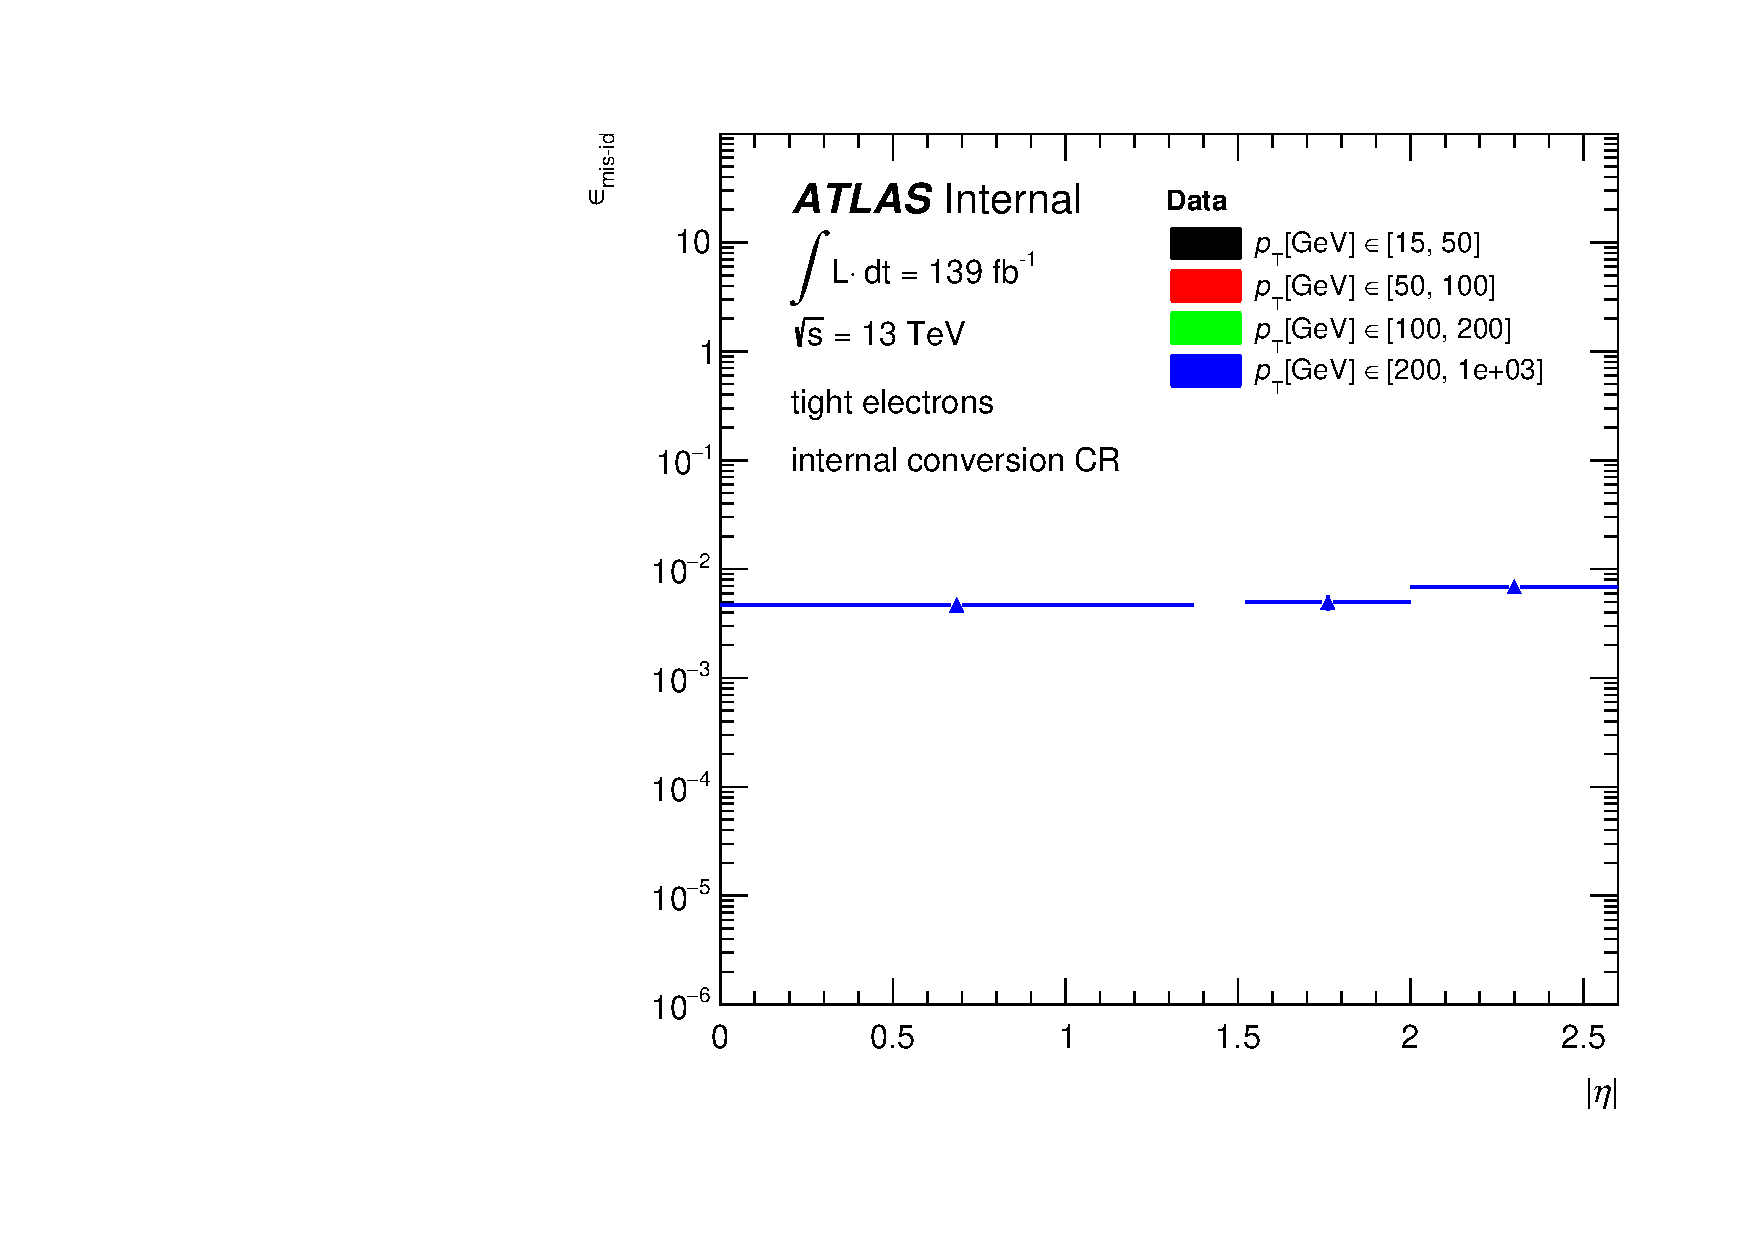
\includegraphics[width=0.32\textwidth]{figures/qmisid/crateData_tight_m0}}
  {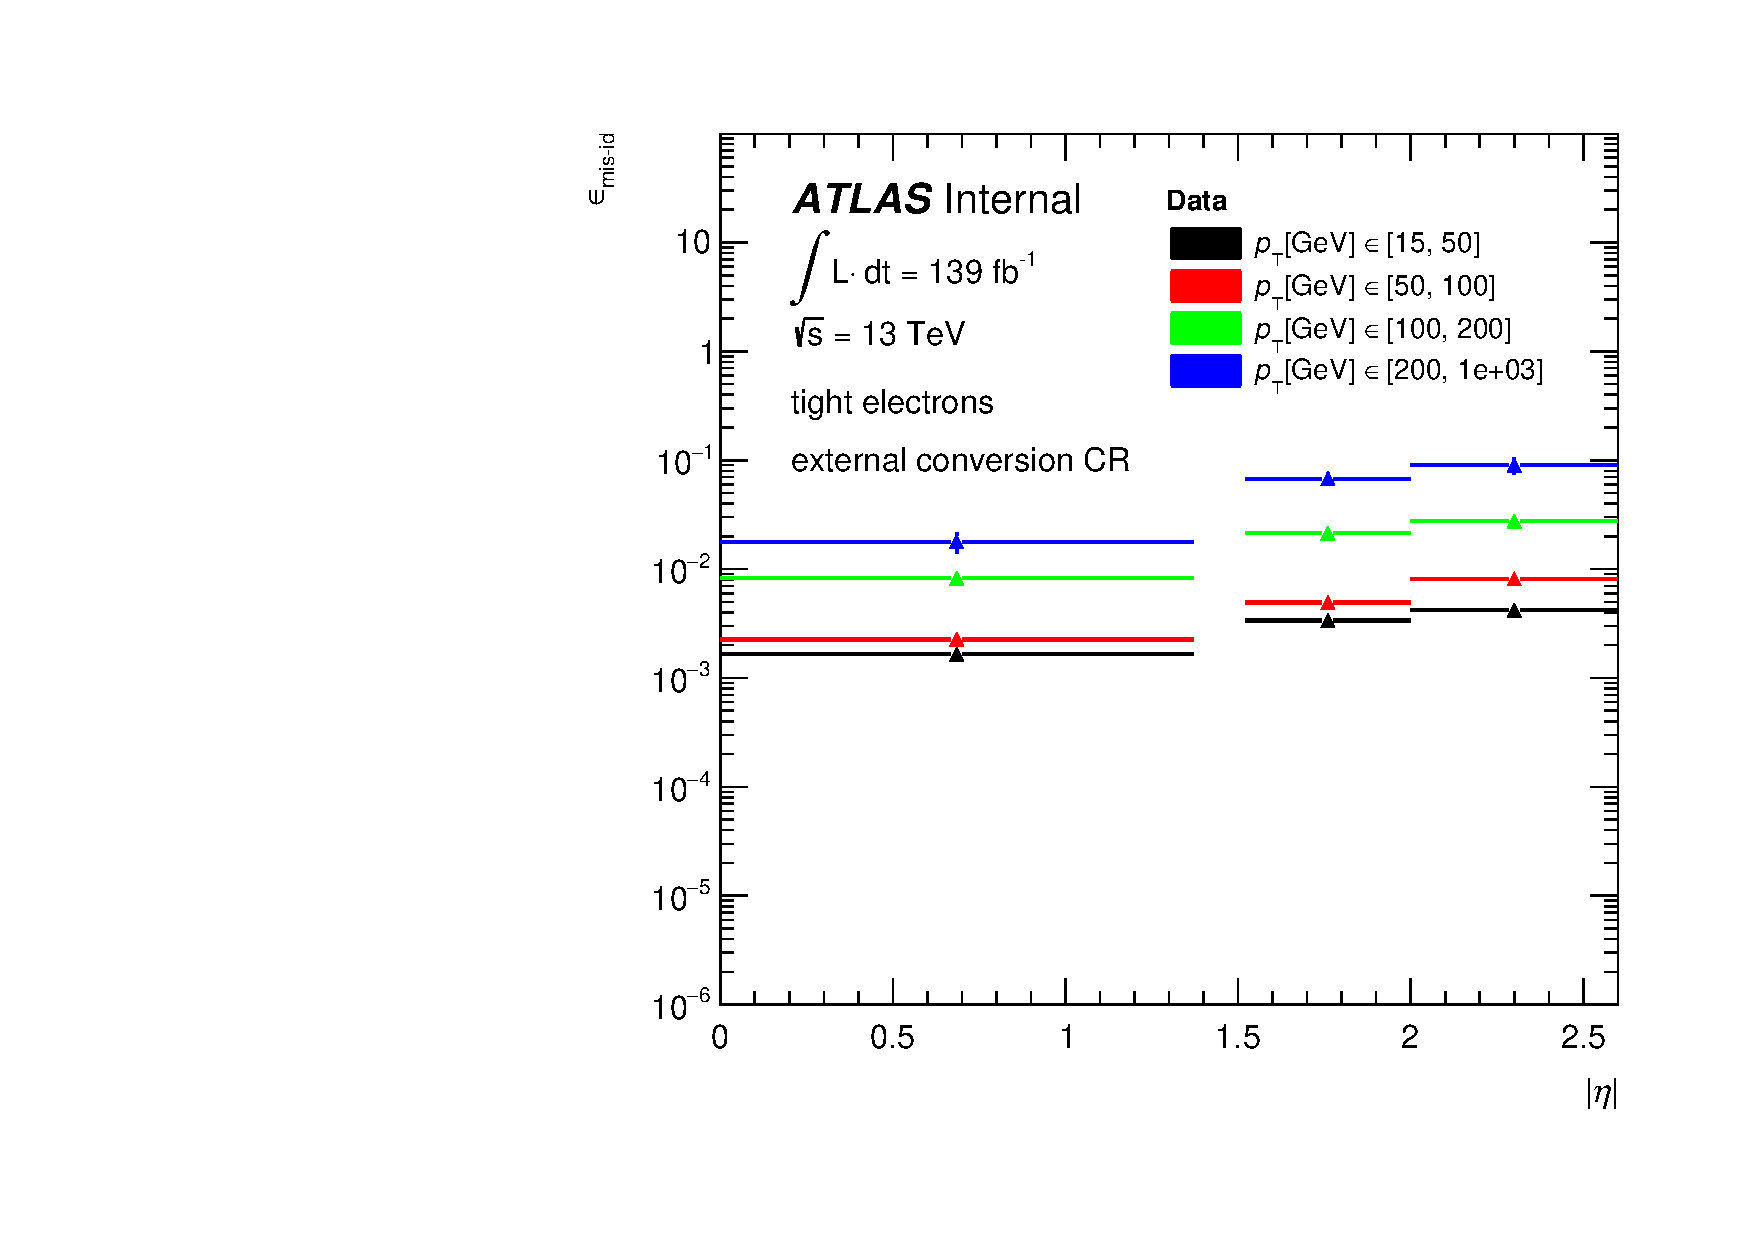
\includegraphics[width=0.32\textwidth]{figures/qmisid/crateData_tight_m1}}
  {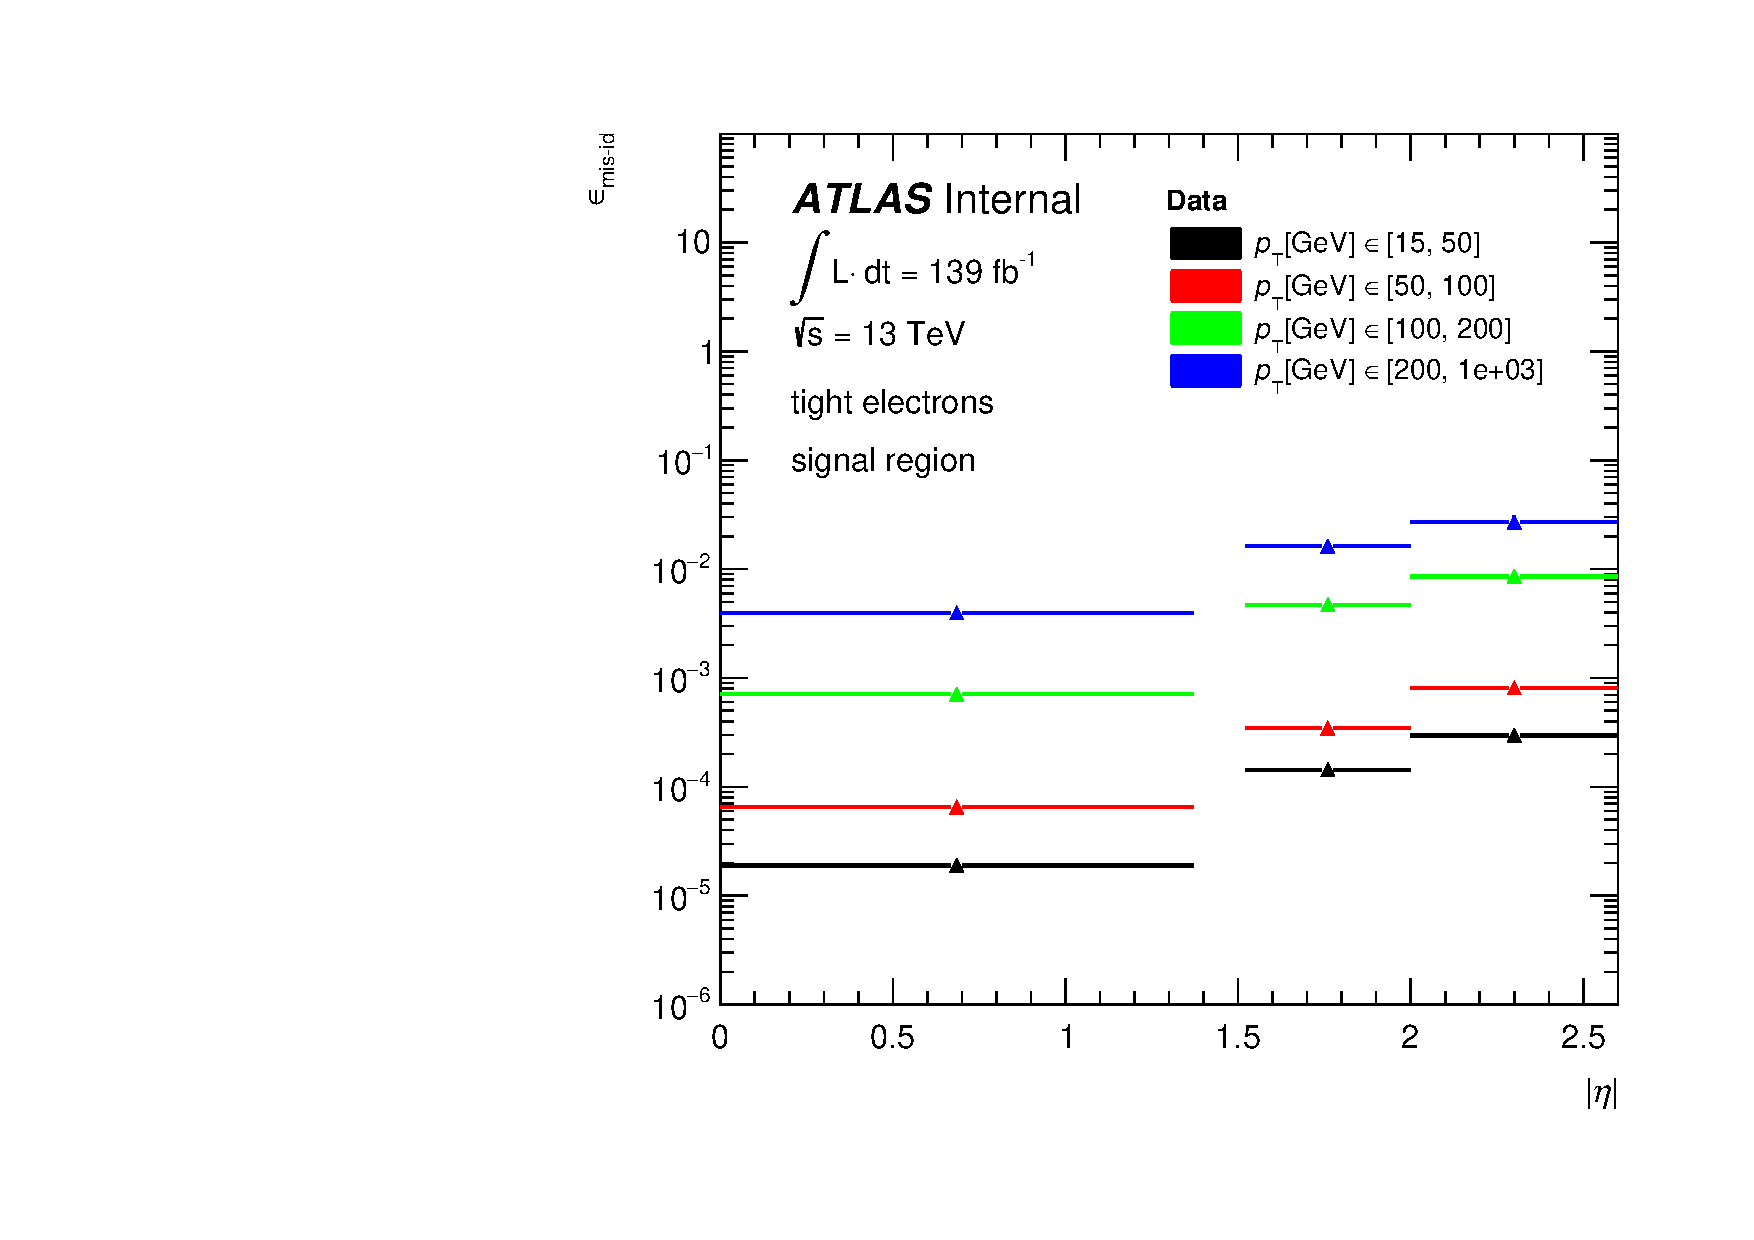
\includegraphics[width=0.32\textwidth]{figures/qmisid/crateData_tight_m2}}
  \caption{Electron charge-flip rates derived from the data with the likelihood method. The rates are presented 
           as a function of $|\eta|$, parameterised in $\pT$ for (a) internal-conversion (b) external-conversion 
           and (c) prompt candidates.\label{fig:Lik2Ddata_main}}
\end{figure}

\begin{figure}[htp!] 
  \centering
  {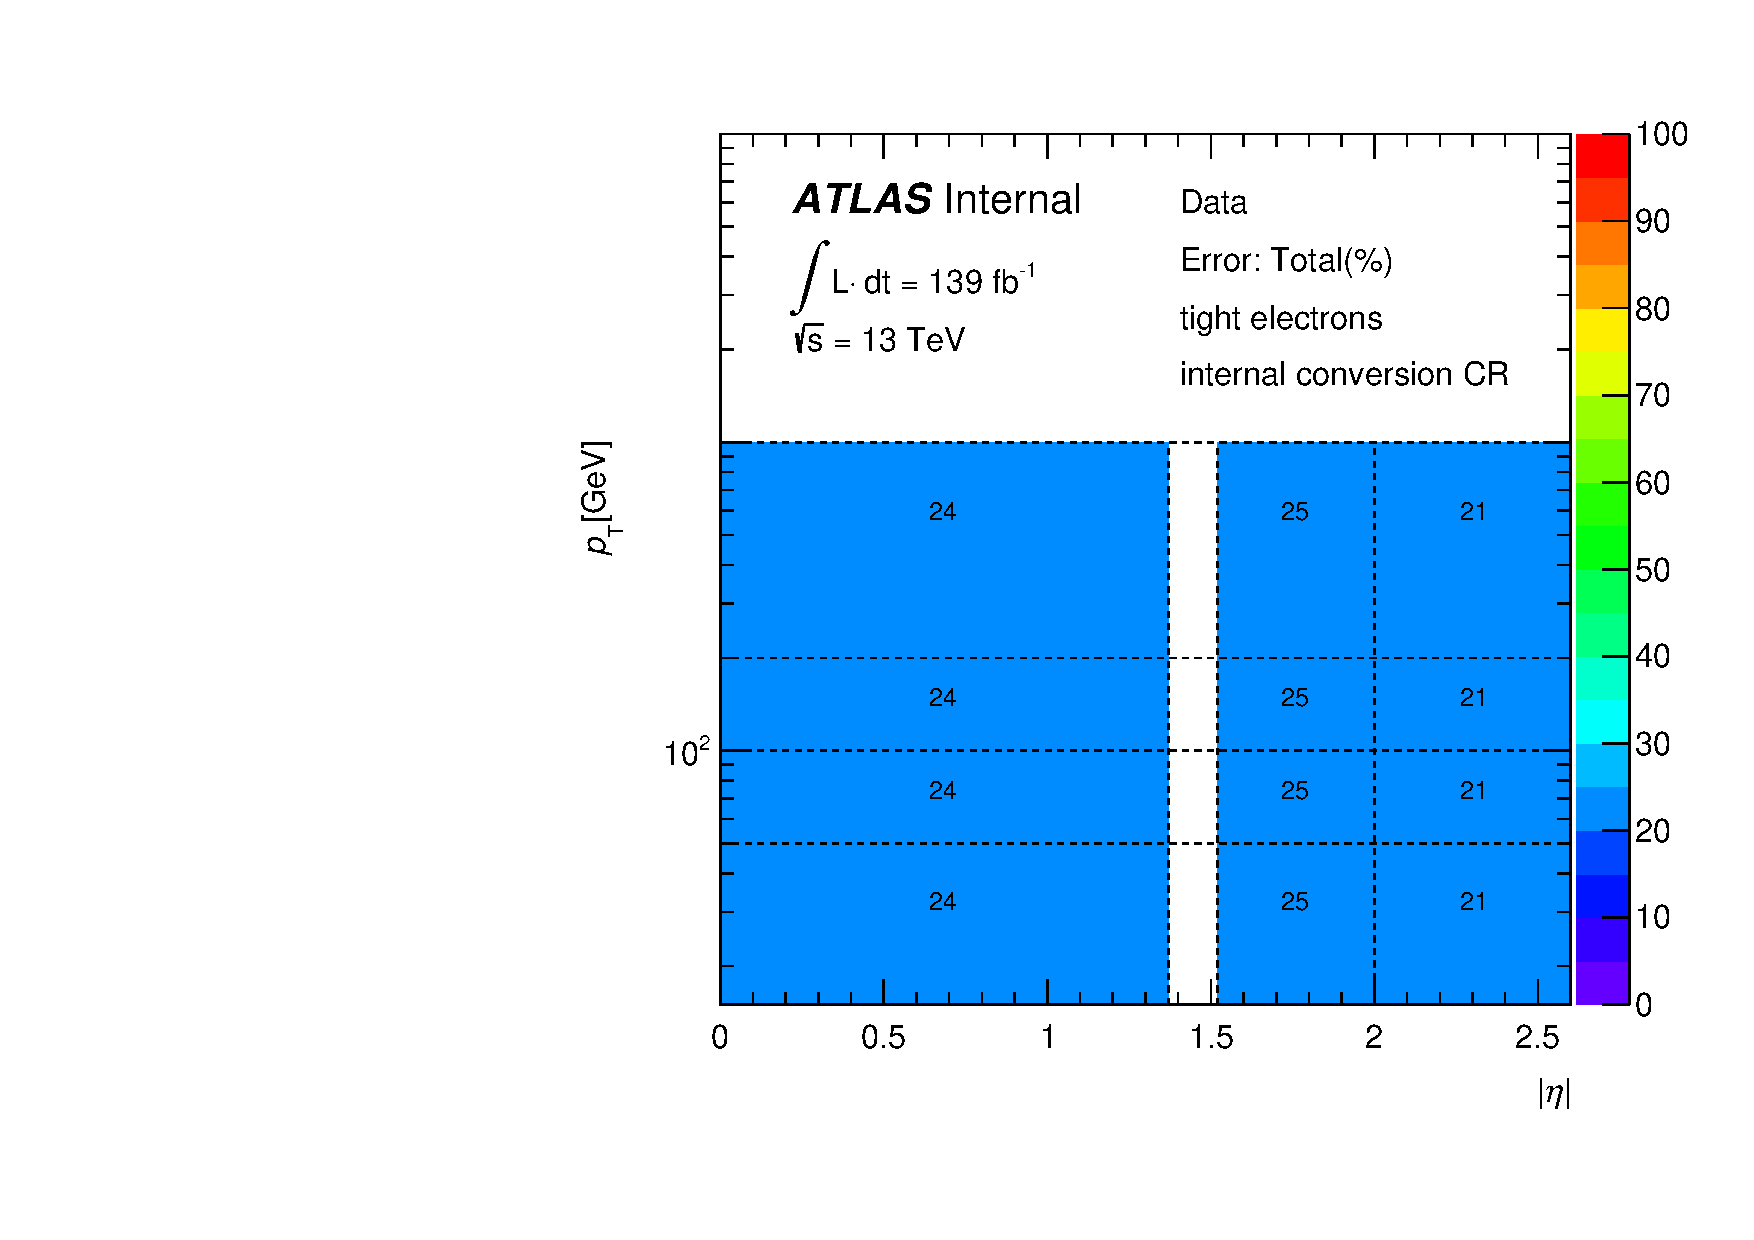
\includegraphics[width=0.32\textwidth]{figures/qmisid/syst_Data_Total_tight_intcr}}
  {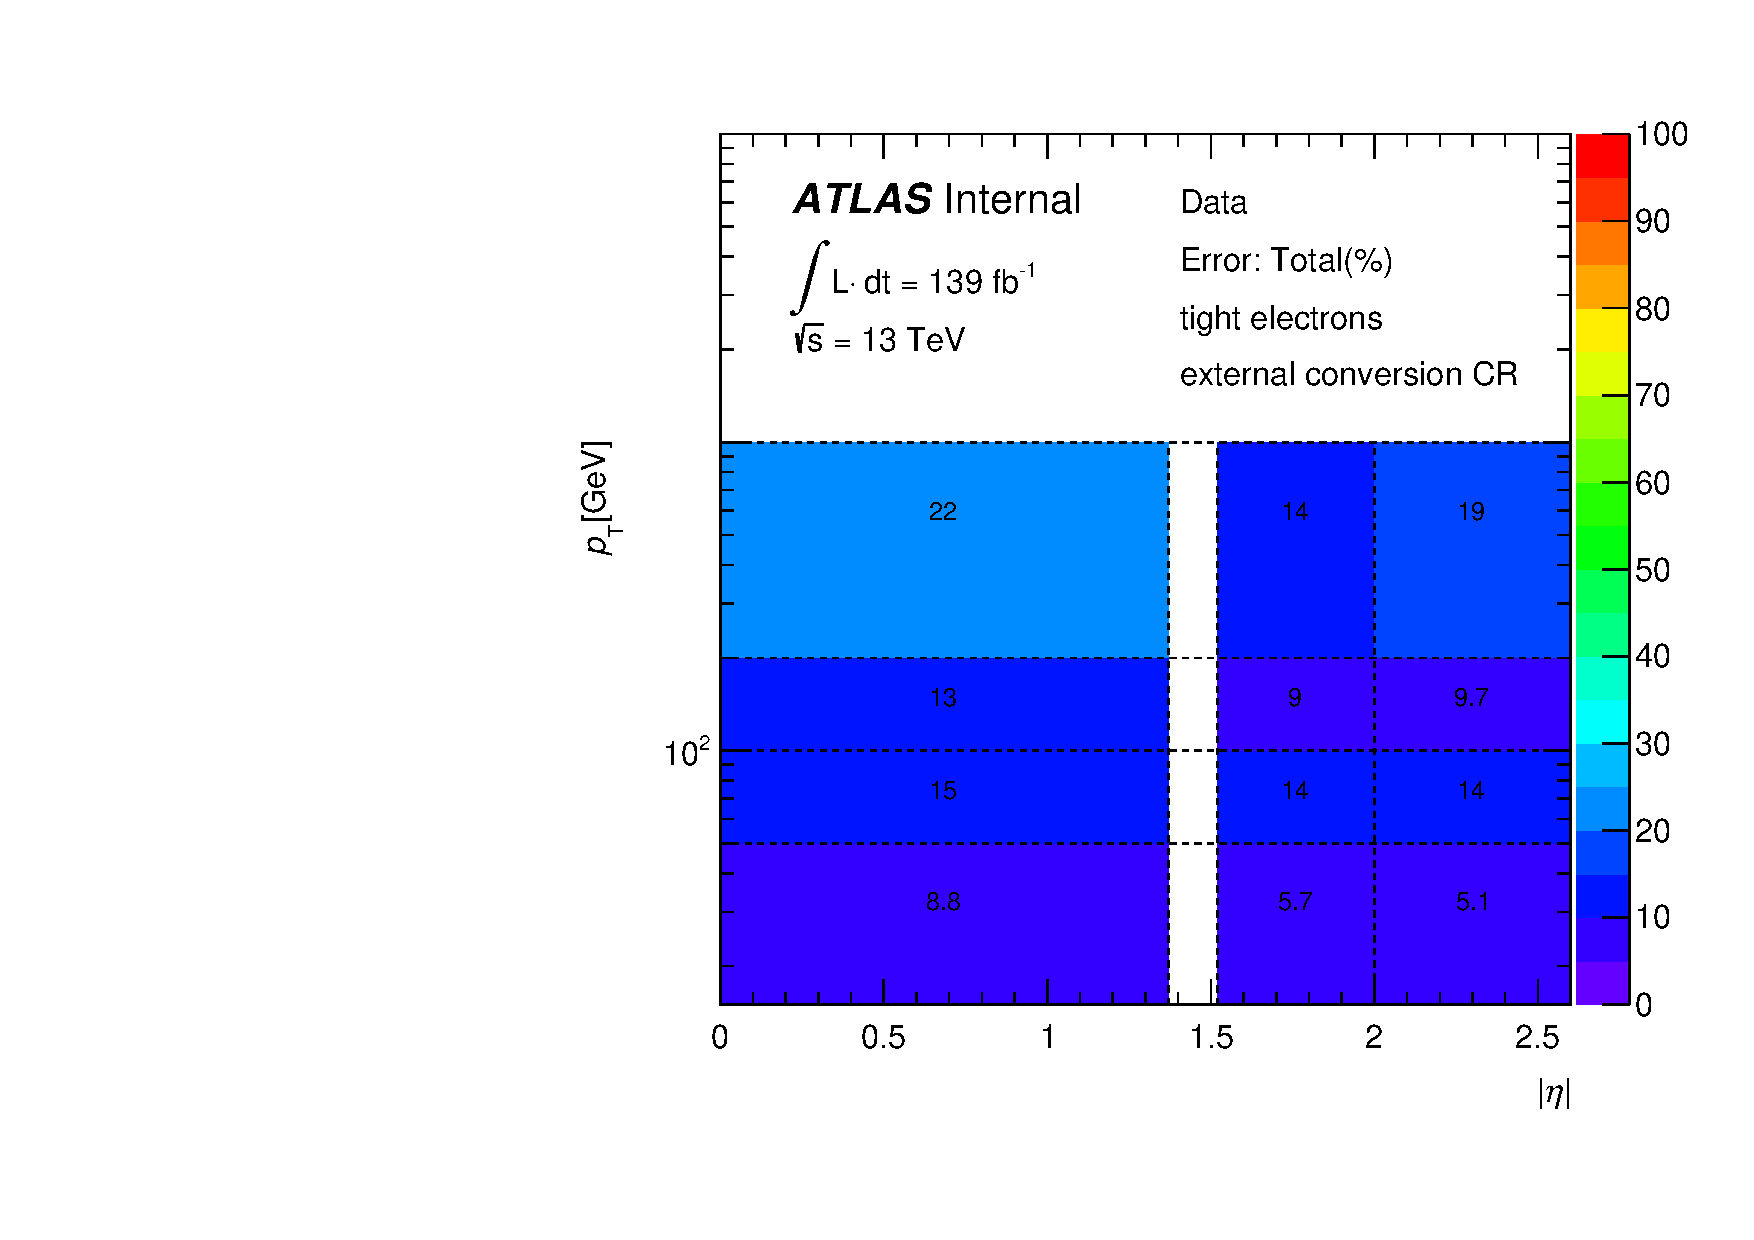
\includegraphics[width=0.32\textwidth]{figures/qmisid/syst_Data_Total_tight_extcr}}
  {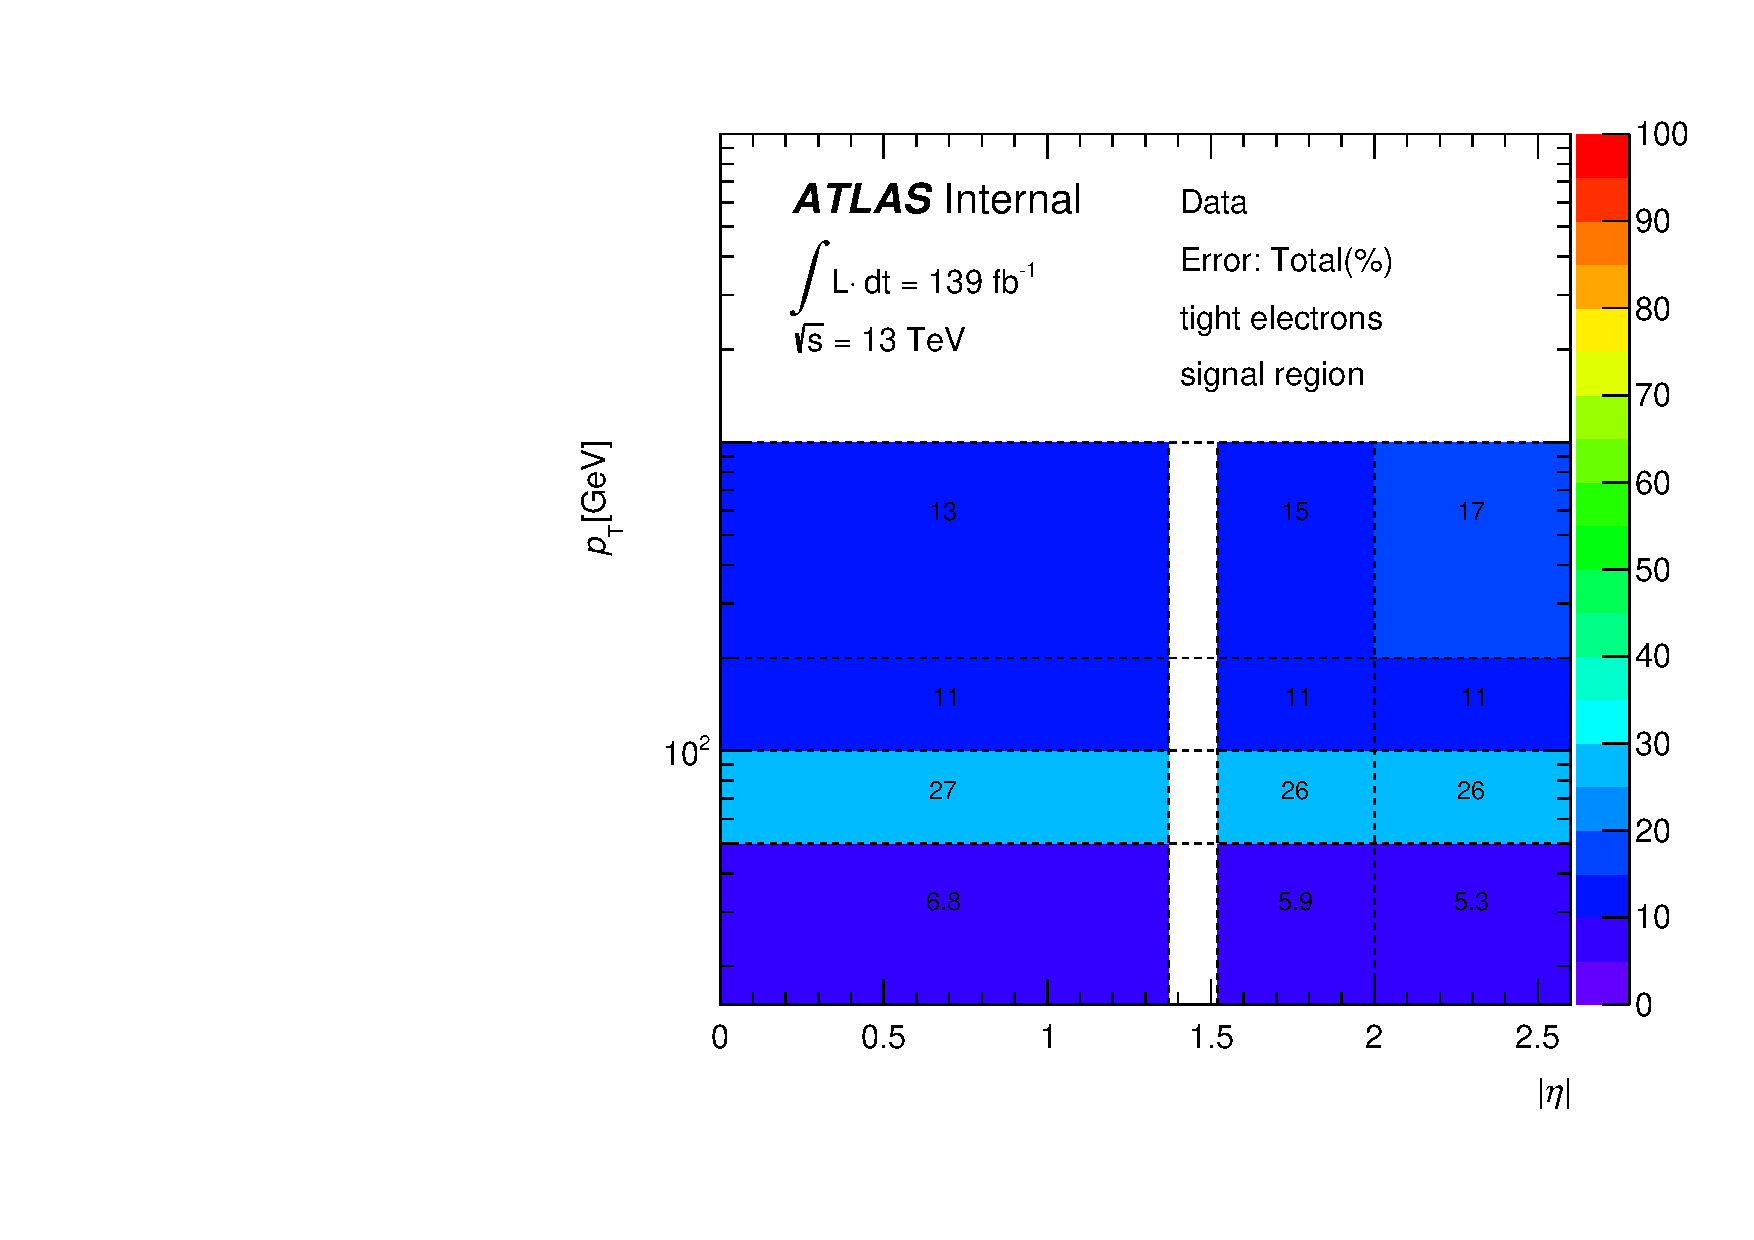
\includegraphics[width=0.32\textwidth]{figures/qmisid/syst_Data_Total_tight_sr}}
  \caption{Total relative systematic uncertainty (in \%) on the charge-flip rate in bins of $|\eta|$ and 
           $\pT$ for (a) internal-conversion (b) external-conversion and (c) prompt electron candidates.
           \label{fig:QMisID:systtight1} }
\end{figure}

Event yields with charge flip electrons are obtained by weighing pre-selected events but asking for 
opposite-sign lepton instead of same-sign. The event weights ($w_{QmisID}$) are defined as:
with the expression:
\begin{equation}
w_{QmisID} = \frac{\epsilon_{\textrm{mis id},1} + \epsilon_{\textrm{mis id},2} - 2\epsilon_{\textrm{mis id},1}\epsilon_{\textrm{mis id},2}}{1-(\epsilon_{\textrm{mis id},1} + \epsilon_{\textrm{mis id},2} - 2\epsilon_{\textrm{mis id},1}\epsilon_{\textrm{mis id},2})}
\label{eq:QmisID_weight}
\end{equation}

where $\epsilon_{\textrm{mis id},1}(1-\epsilon_{\textrm{mis
    id},2})+\epsilon_{\textrm{mis id},2}(1-\epsilon_{\textrm{mis id},1}) =
\epsilon_{\textrm{mis id},1} + \epsilon_{\textrm{mis id},2} -
2\epsilon_{\textrm{mis id},1}\epsilon_{\textrm{mis id},2}$ is the rate of
events in which exactly one electron is reconstructed with charge flip.
In order to account for the strong dependence of the rates to the $\pT$ and to
improve the modeling of the kinematical observables, $\pT$ continuous rates are used.

\subsection{Electron charge flip background study}

The following paragraphs present the measurement of the background, introduced to final states with two 
same-sign light leptons ($e^{\pm}e^{\pm}$, $e^{\pm}\mu^{\pm}$) due to electron charge misidentification 
(QMisID).\footnote{Unless specified otherwise, positrons and electrons are both called electrons.} There 
are two main mechanisms contributing to QMisID:
%
\begin{itemize}
  \item Hard Bremsstrahlung ($e^\pm \rightarrow e^\pm \gamma^* \rightarrow e^\pm e^+e^-$). In this 
  case, QMisID occurs when the EM cluster is coupled to the track of the opposite-sign electron 
  in the trident. Since the probability of this process depends on the traversed detector material, 
  dependence of the QMisID rate on $|\eta|$ is expected.
  \item Mismeasurement of the electron track-curvature. This effect is more important in the high 
  $p_{\mathrm T}$ range (smaller curvature), therefore dependence of the rate on $p_{\mathrm T}$ 
  is also expected.
\end{itemize}
%
The misidentification of the muon charge-sign is not considered in this study. It may occur by mismeasurement 
of the track curvature, however, due to the long lever arm in the muon system and the fact that the charge is 
measured both in the inner detector and the muon spectrometer, the QMisID rate is marginal.

The estimation of the QMisID background is based on the electron QMisID rates $\vec{\epsilon}$. The latter 
are derived from the data, in three-dimensional (3D) bins according to $|\eta|$, $p_{\mathrm T}$ and the 
region to which the electron belongs with respect to photon conversions, i.e. it designated as internal- 
or external-conversion candidate or as prompt lepton (as defined in the
same-sign signal region).



%~~~~~~~~~~~~~~~~~~~~~~~~~~~~~~~~~~~
\subsubsection{Background estimation strategy} 
%~~~~~~~~~~~~~~~~~~~~~~~~~~~~~~~~~~~
Final states with an opposite-sign lepton pair (mainly $Z \rightarrow e^+e^- $
followed by $t\bar{t} \rightarrow b\bar{b}W^+W^- \rightarrow b\bar{b}e^+e^-\nu\bar{\nu}$)
contaminate the signal region, defined by two same-sign leptons, when the charge of exactly one lepton
is misidentified. In the case of $e^{-}e^{+}$, the fraction of events that are reconstructed as same-sign 
($e^{-}e^{-}$ or $e^{+}e^{+}$) is:
%
\begin{equation}
  \epsilon_i(1-\epsilon_j) + \epsilon_j(1-\epsilon_i) = \epsilon_i +\epsilon_j - 2\epsilon_i\epsilon_j, 
\end{equation}
%
where $\epsilon_i$ and $\epsilon_j$ are the QMisID rates for each of the two electrons. For $e^{\pm}\mu^{\mp}$ 
events, on the other hand, the respective fraction is equal to the QMisID rate $\epsilon_i$ of the electron. 
By knowing the QMisID rates it is thereby possible to compute the expected number of misidentified same-sign 
events $\bar{N}_\mathrm{SS}$ from the observed number of opposite-sign events $N_\mathrm{OS}$, using the expressions:
%
\begin{equation}
  \bar{N}_\mathrm{SS} = \frac{\epsilon_i +\epsilon_j -2\epsilon_i \epsilon_j}{1-(\epsilon_i +\epsilon_j -2\epsilon_i \epsilon_j)} N_\mathrm{OS}
  \hspace{10pt}\text{and}\hspace{10pt}
  \bar{N}_\mathrm{SS} = \frac{\epsilon_i}{1-\epsilon_i} N_\mathrm{OS}
\end{equation}
%
for the $ee$ and $e\mu$ channel, respectively.

%~~~~~~~~~~~~~~~~~~~~~~~~~~~~~~~~~~~
\subsubsection{Estimation of the charge mis-identification rates with the likelihood method} 
%~~~~~~~~~~~~~~~~~~~~~~~~~~~~~~~~~~~
The QMisID rates are derived from the data, based on the fraction of $Z\rightarrow ee$ decays that are reconstructed 
as a same-sign electron pair. For this measurement, events in the $m_{ee}$ region around the reconstructed $Z$-boson 
peak $m_Z$ are used. For $N^{ij}$ electron pairs falling in the bin combination $i,j$ (where each of $i,j$ uniquely 
represents a 3D bin as defined above) the expected number of same-sign events is:
%
\begin{equation}
  \label{app:eq:qmisid1}
  \bar{N}^{ij}_\mathrm{SS}(\epsilon_i,\epsilon_j)=N^{ij}\cdot(\epsilon_i+\epsilon_j-2\epsilon_i\epsilon_j).
\end{equation}
%
Asumming that all of the observed same-sign events, $N^{ij}_\mathrm{SS}$, in the $m_Z$ window are products 
of electron charge mis-identification, they follow a Poisson distribution around the expectation value:
%
\begin{equation}
\label{app:eq:qmisid2}
  f(N^{ij}_\mathrm{SS}|\bar{N}_\mathrm{SS}(\epsilon_i,\epsilon_j))=\frac{[{\bar{N}}^{ij}_\mathrm{SS}]^{N^{ij}_\mathrm{SS}} e^{-{\bar{N}}^{ij}_\mathrm{SS}}}{N^{ij}_\mathrm{SS}!}.
\end{equation}

which is integrated into a likelihood:
%
\begin{equation}
  L(\vec{\epsilon}|N_\mathrm{SS})=\prod_{i,j}f(N^{ij}_\mathrm{SS}|\bar{N}_\mathrm{SS}(\epsilon_i,\epsilon_j)).
\end{equation}
%
that can be maximised (minimisation of $-2\ln L$) to obtain the rates that best describe the data. 

As mentioned above, this method relies on the assumption that $ee$ events in the $m_Z$ window are products of $Z$-boson decays. 
Therefore, any contribution from other processes (e.g. fake electrons) to $N^{ij}_\mathrm{SS}$ must be subtracted. As long as 
these processes do not exhibit a resonant-like behaviour of the $m_{ee}$ distribution, this background can be estimated from 
the sidebands of the $m_{Z}$ window, for each bin combination $i,j$, separately for same-sign ($N^{ij}_\mathrm{SS,BG}$) and 
opposite-sign ($N^{ij}_\mathrm{OS,BG}$) events. For this, upper and lower sidebands are defined with width equal to the $m_{Z}$ 
window so that the introduced background can be obtained from the average yield. The background estimate is then used to correct 
the expectation (equation\,\ref{app:eq:qmisid1}) to:
%
\begin{equation}
  \bar{N}^{ij}_\mathrm{SS} = N^{ij}_\mathrm{SS,BG} + (N^{ij}-N^{ij}_\mathrm{SS,BG}-N^{ij}_\mathrm{OS,BG})\cdot(\epsilon_i+\epsilon_j-2\epsilon_i\epsilon_j).
\end{equation}
%
The minimisation of $-2\ln L$ is finally performed by MIGRAD, while HESSE is called to evaluate the uncertainty on the 
rate estimates. 

%~~~~~~~~~~~~~~~~~~~~~~~~~~~~~~~~~~~
\subsubsection{Data and Monte Carlo samples}
\label{sec:qmisiddata}
%~~~~~~~~~~~~~~~~~~~~~~~~~~~~~~~~~~~

The QMisID rate and background estimation is performed using the full dataset, with an integrated luminosity 
of 139\,fb$^{-1}$. For the validation of the method and many of the tests that follow, 
simulated $Z\to ee$ ({\scshape Sherpa}), $t\bar{t}$ (\textsc{Powheg-BOX}) and $t\bar{t}\gamma$ (\textsc{MG5\_aMC}) samples 
are also used.

No additional criteria are applied to electrons for the QMisID rate
estimation. In order to increase the size of the tight electron sample,
anti-tight electrons are also exploited.  
The latter are defined as those electrons that fail the tight identification criteria but yet pass the overlap removal. Although such 
electrons are not used in the analysis, by using a looser set of electrons and classifying them as tight and anti-tight (on top of the 
3D classification described above), introduces events with one tight and one anti-tight electron in the rate estimation, and therefore 
improves the statistical precision of the tight-electron rates with the likelihood method.

%~~~~~~~~~~~~~~~~~~~~~~~~~~~~~~~~~~~~~~~~~~~~~~~~~~~~~~~~~~~~~~~~~~~~~~~~~~
\subsubsection{$M_{ee}$ sidebands for $Z\rightarrow ee$ background estimation}
\label{app:sec:AppQMisIDregions}
%~~~~~~~~~~~~~~~~~~~~~~~~~~~~~~~~~~~~~~~~~~~~~~~~~~~~~~~~~~~~~~~~~~~~~~~~~~

The likelihood method uses $Z\rightarrow ee$ decays with both same-sign and opposite-sign electrons in the final state. As shown 
in figure\,\ref{fig:mlldata}, the $m_{ee}$ distribution of same-sign electrons is shifted towards lower values with respect to 
that of opposite-sign electrons, due to the loss of electron momentum in tridents. To account for this shift, a different $m_Z$ 
window is defined for each case. The $m_Z$ window is determined by gaussian fit around the peak (using all loose electrons) and 
defined as $\pm 4\sigma$ around the mean ($4\sigma$ has been found to provide the best results in terms of closure). The side-bands 
are defined with equal width to the $m_Z$ window, i.e. $8\sigma$ each. The region definitions are summarised in table~\ref{tab:QMisID:Ranges}.
The variation of the rates with the definition of the $m_Z$ window ($\pm 1\sigma$) is considered as a systematic uncertainty.

\smallskip

\begin{table}[h!]
  \begin{center}
    \begin{tabular}{l c c c}
      Sample & lower SB & $m_Z$ window & upper SB \\
      Same-sign & [51.7,76.5] & [76.5,101.3] & [101.3,126.0] \\
      Opposite-sign & [54.7,78.5] & [78.5,102.3] & [102.3,126.0] \\
    \end{tabular}
     \caption{Definition of the $m_Z$ window and side-bands (SB) used in the likelihood method.\label{tab:QMisID:Ranges}}
  \end{center}
\vspace*{-\baselineskip}
\end{table}

\begin{figure}[h!]
  \centering
  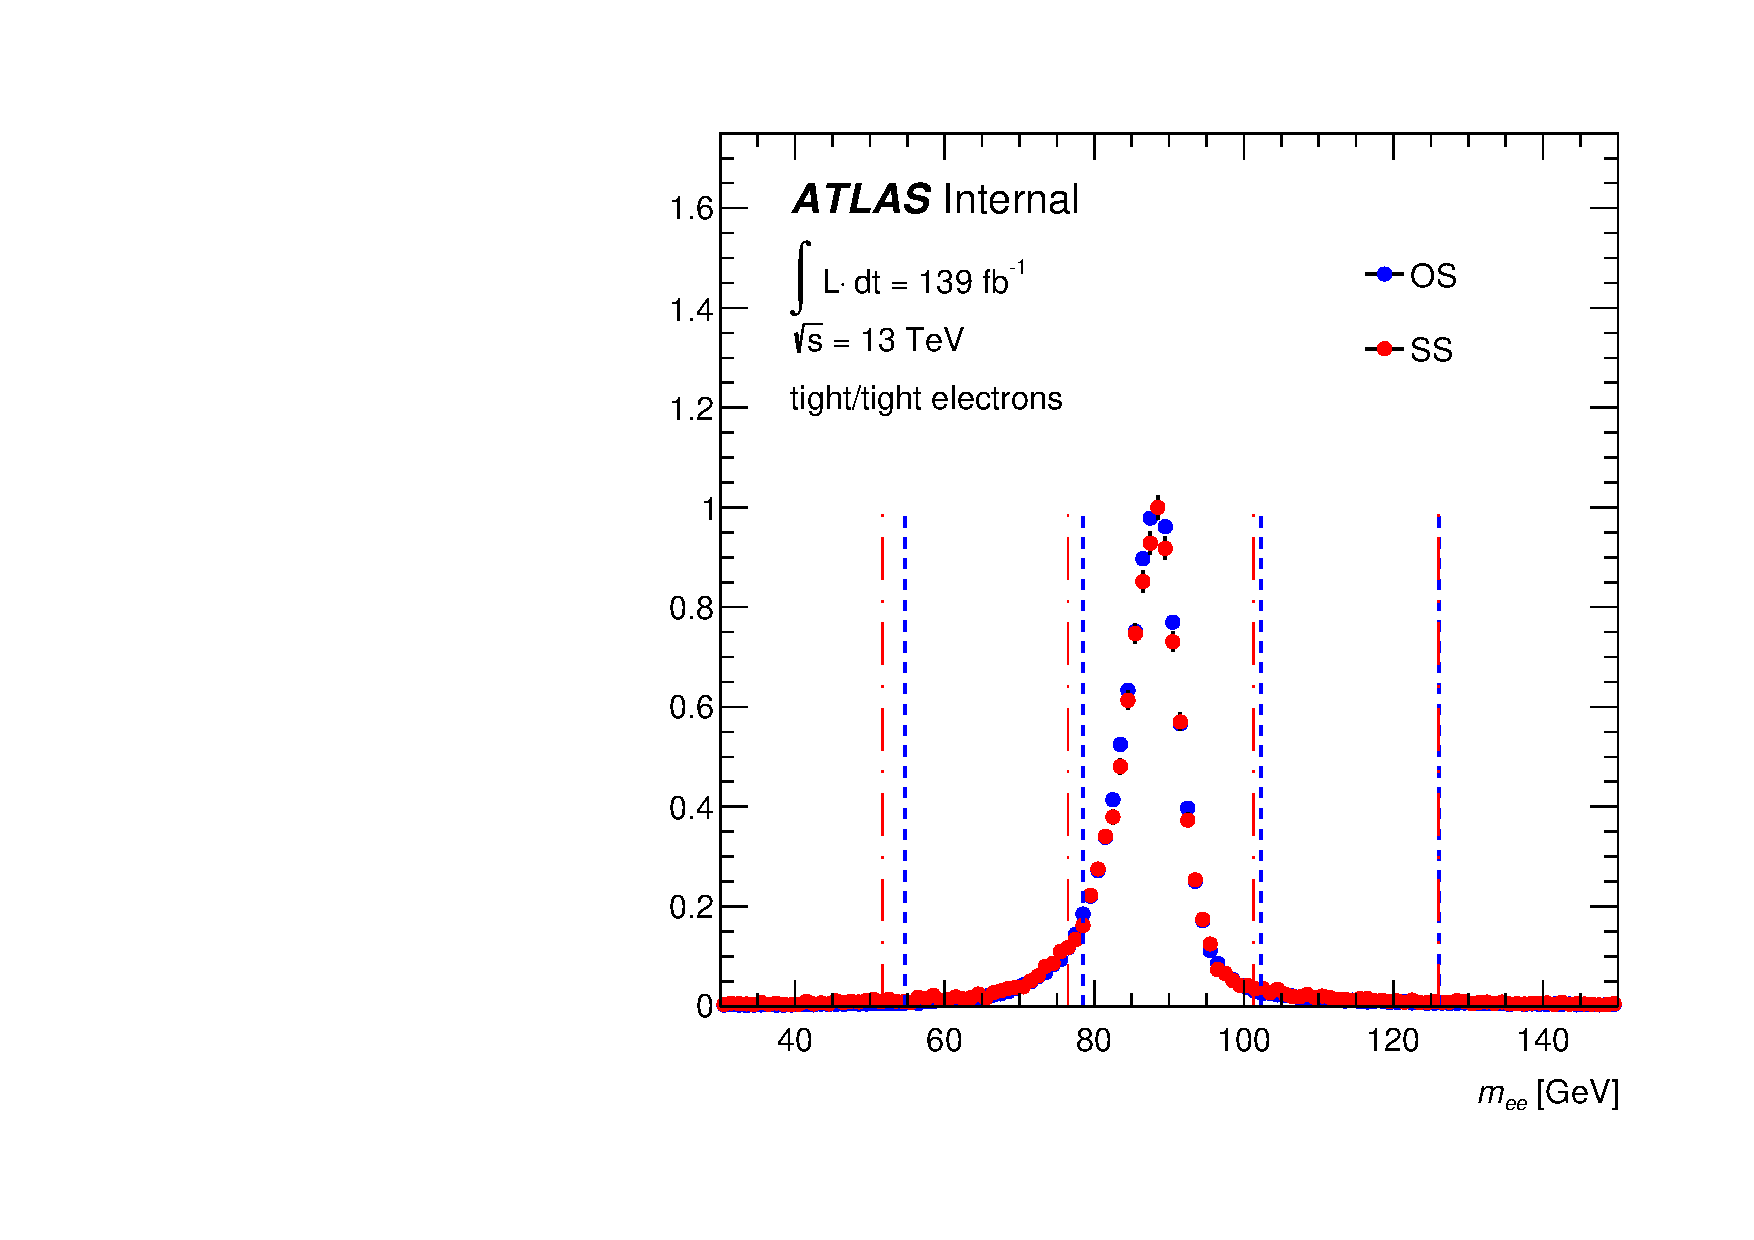
\includegraphics[width=0.45\textwidth]{figures/qmisid/mll_tt}
  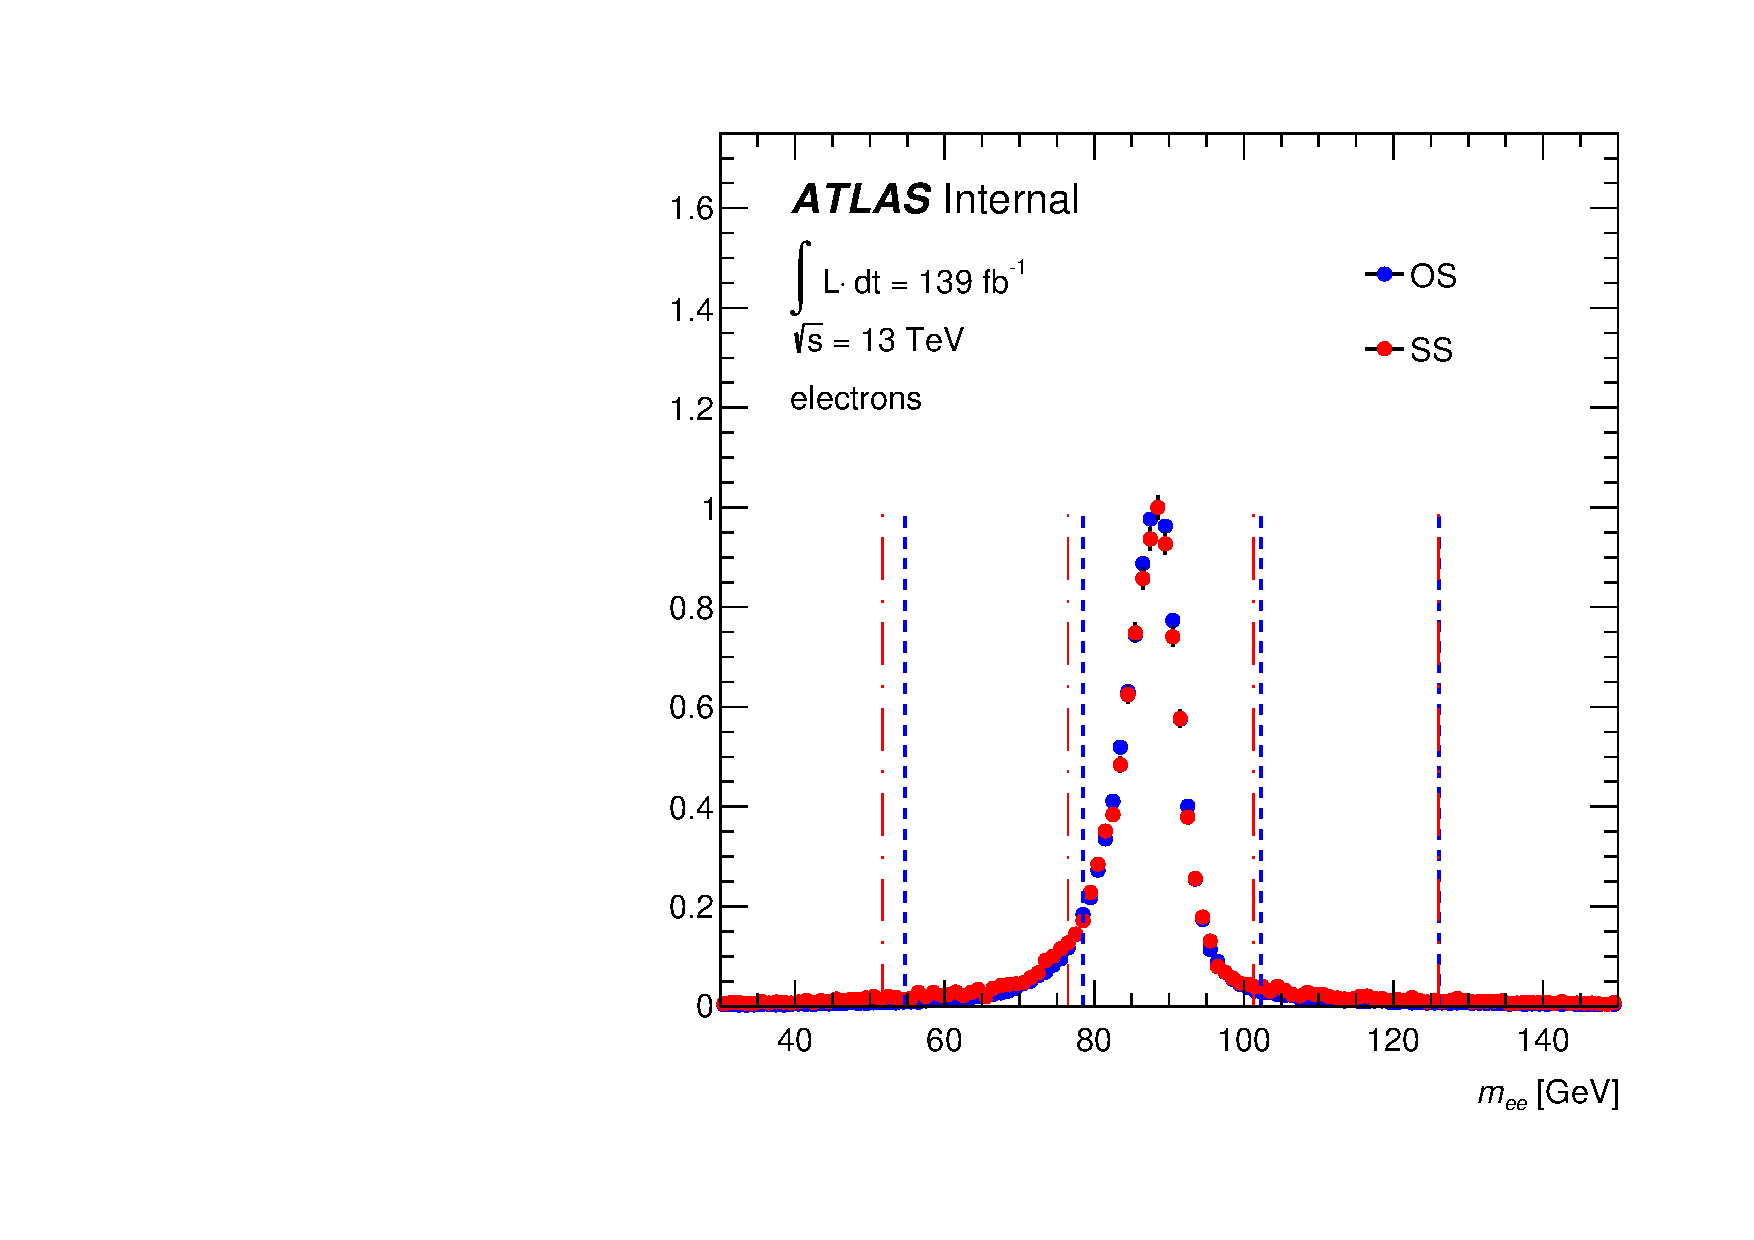
\includegraphics[width=0.45\textwidth]{figures/qmisid/mll_all}
  \caption{Comparison of the $m_{ee}$ distribution between same-sign and opposite-sign data events for pairs of 
  (a) tight and (b) loose electrons. The distributions are 
  normalized by the maximum value. The peak for same-sign electrons is shifted with respect to opposite-sign 
  electrons due to the loss of electron momentum in tridents.\label{fig:mlldata}}
\end{figure}

%~~~~~~~~~~~~~~~~~~~~~~~~~~~~~~~~~~~~~~~~~~~~~~~~~~~~~~~~~~~~~~~~~
\subsubsection{Data-driven rates estimates with $\pT$ continuous rates}
%~~~~~~~~~~~~~~~~~~~~~~~~~~~~~~~~~~~~~~~~~~~~~~~~~~~~~~~~~~~~~~~~~

The binning in $|\eta|$ and $\pT$ must be optimised to best describe the dependence of the rates on each quantity
while maintaing statistical precision.

The binning scheme 
distinguishes four bins in $|\eta|$ 
(one of which just isolates the crack region) and four bins in $\pT$, for each region w.r.t. to photon conversions. 
To mitigate the statistical uncertainties introduced by the size of the available dataset in the case of 
tight-electrons, $\pT$ bins are merged in the case of the internal conversion control region (merging is 
implemented by assigning the same rate in the likelihood).
The data-driven QMisID rates, derived with the above binning configuration, are presented in figure\,\ref{fig:Lik2Ddata}.

Figure\,\ref{fig:DatapTJumps}(a) shows the expected $\pT$ distribution in the
data, using reweighted opposite-sign events, compared to the
observation. Significant non closures are observed at the edges of the $\pT$
bins. These non-closures are covered by the non-closure systematic
uncertainties in average only. The local non-closures exceed significantly the
systematic uncertainties. They can of $200\%$ in the 60-80~GeV range, and higher
than $200\%$ in the 150-200~GeV ranges.
 
In order to control this effect, $\pT$ continuous modeling of the rates is
used. The effective rate at a given $\pT$ is obtained by the weighted
sum of the rates from the adjacend $\pT$ bins. The weighting is based on
$\pT$ only and accounts for the $\pT$ disctribution shape.

\begin{figure}[htb!]
\centering
  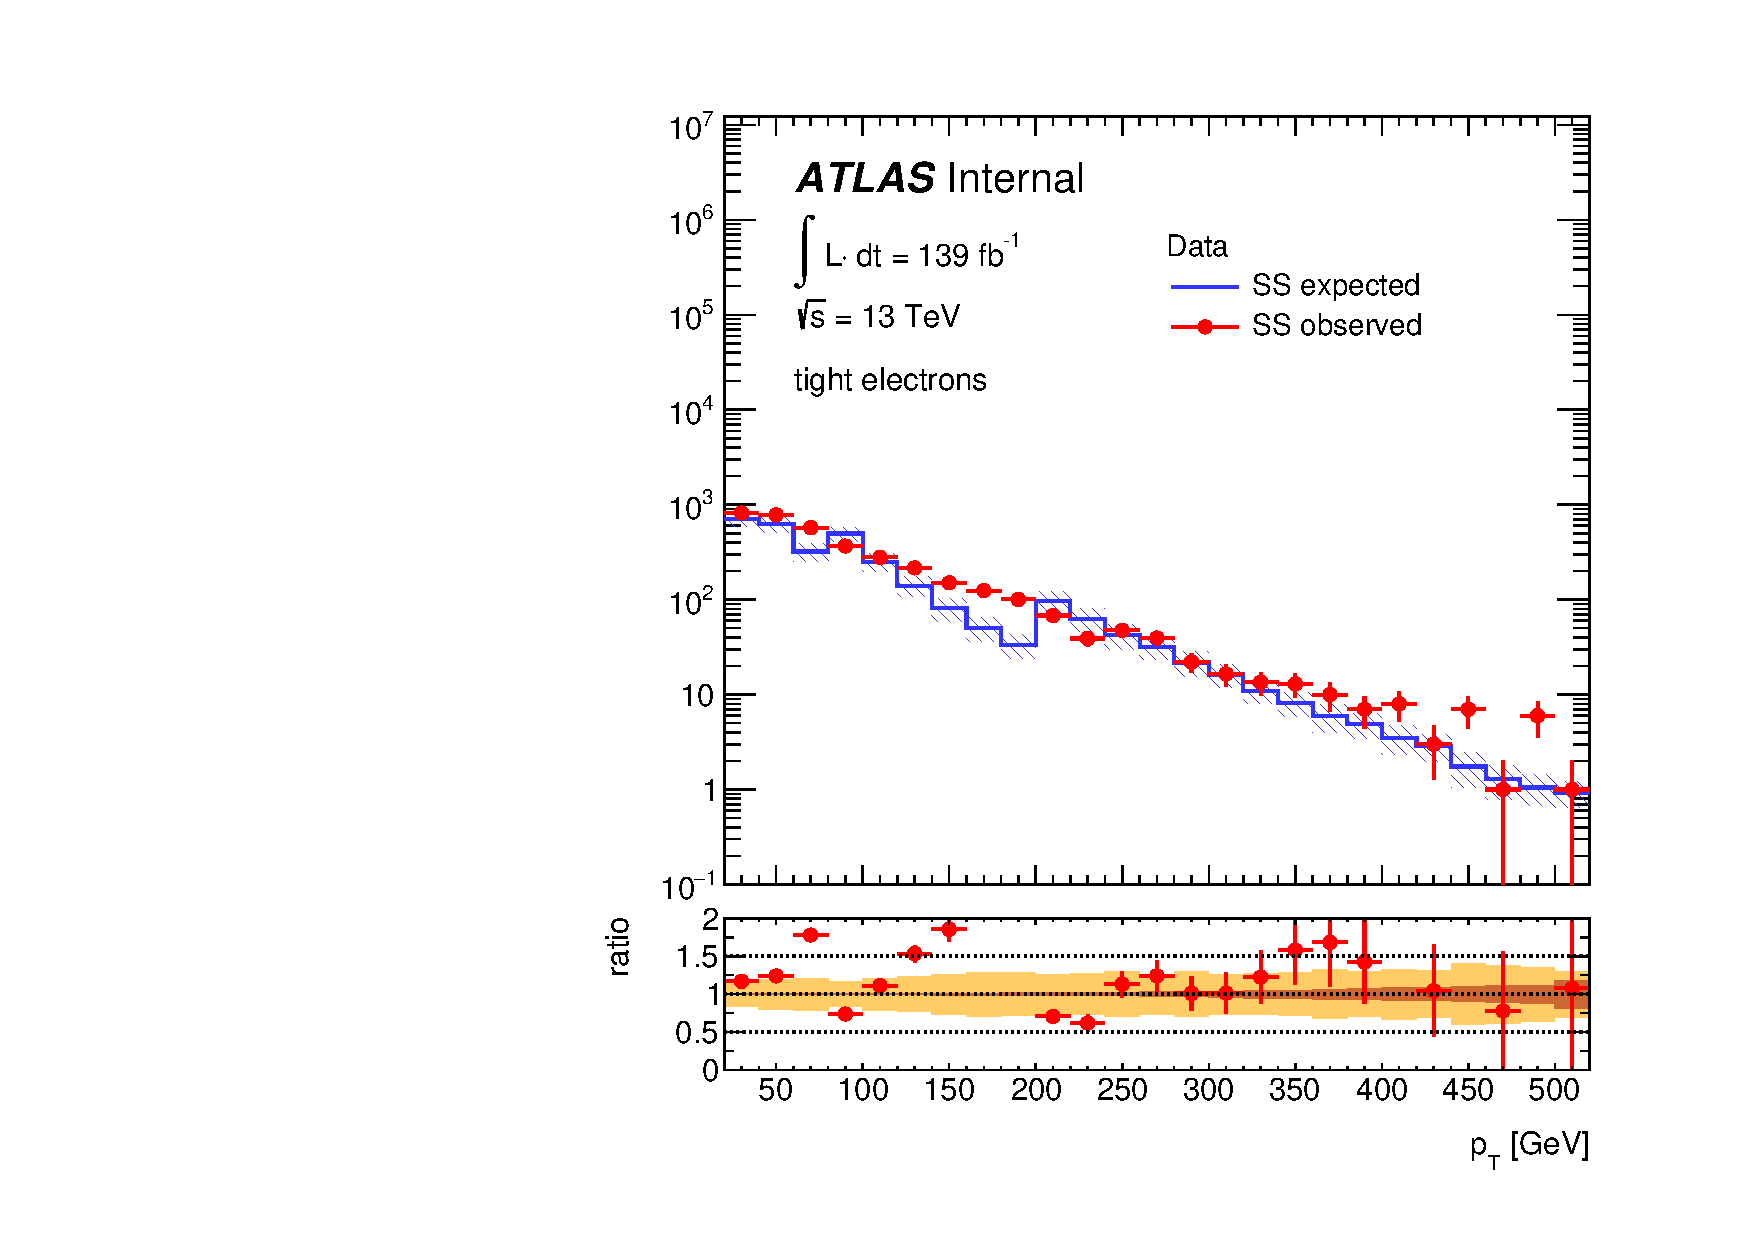
\includegraphics[width=0.45\textwidth]{figures/qmisid/valid_PttightData_binned}
  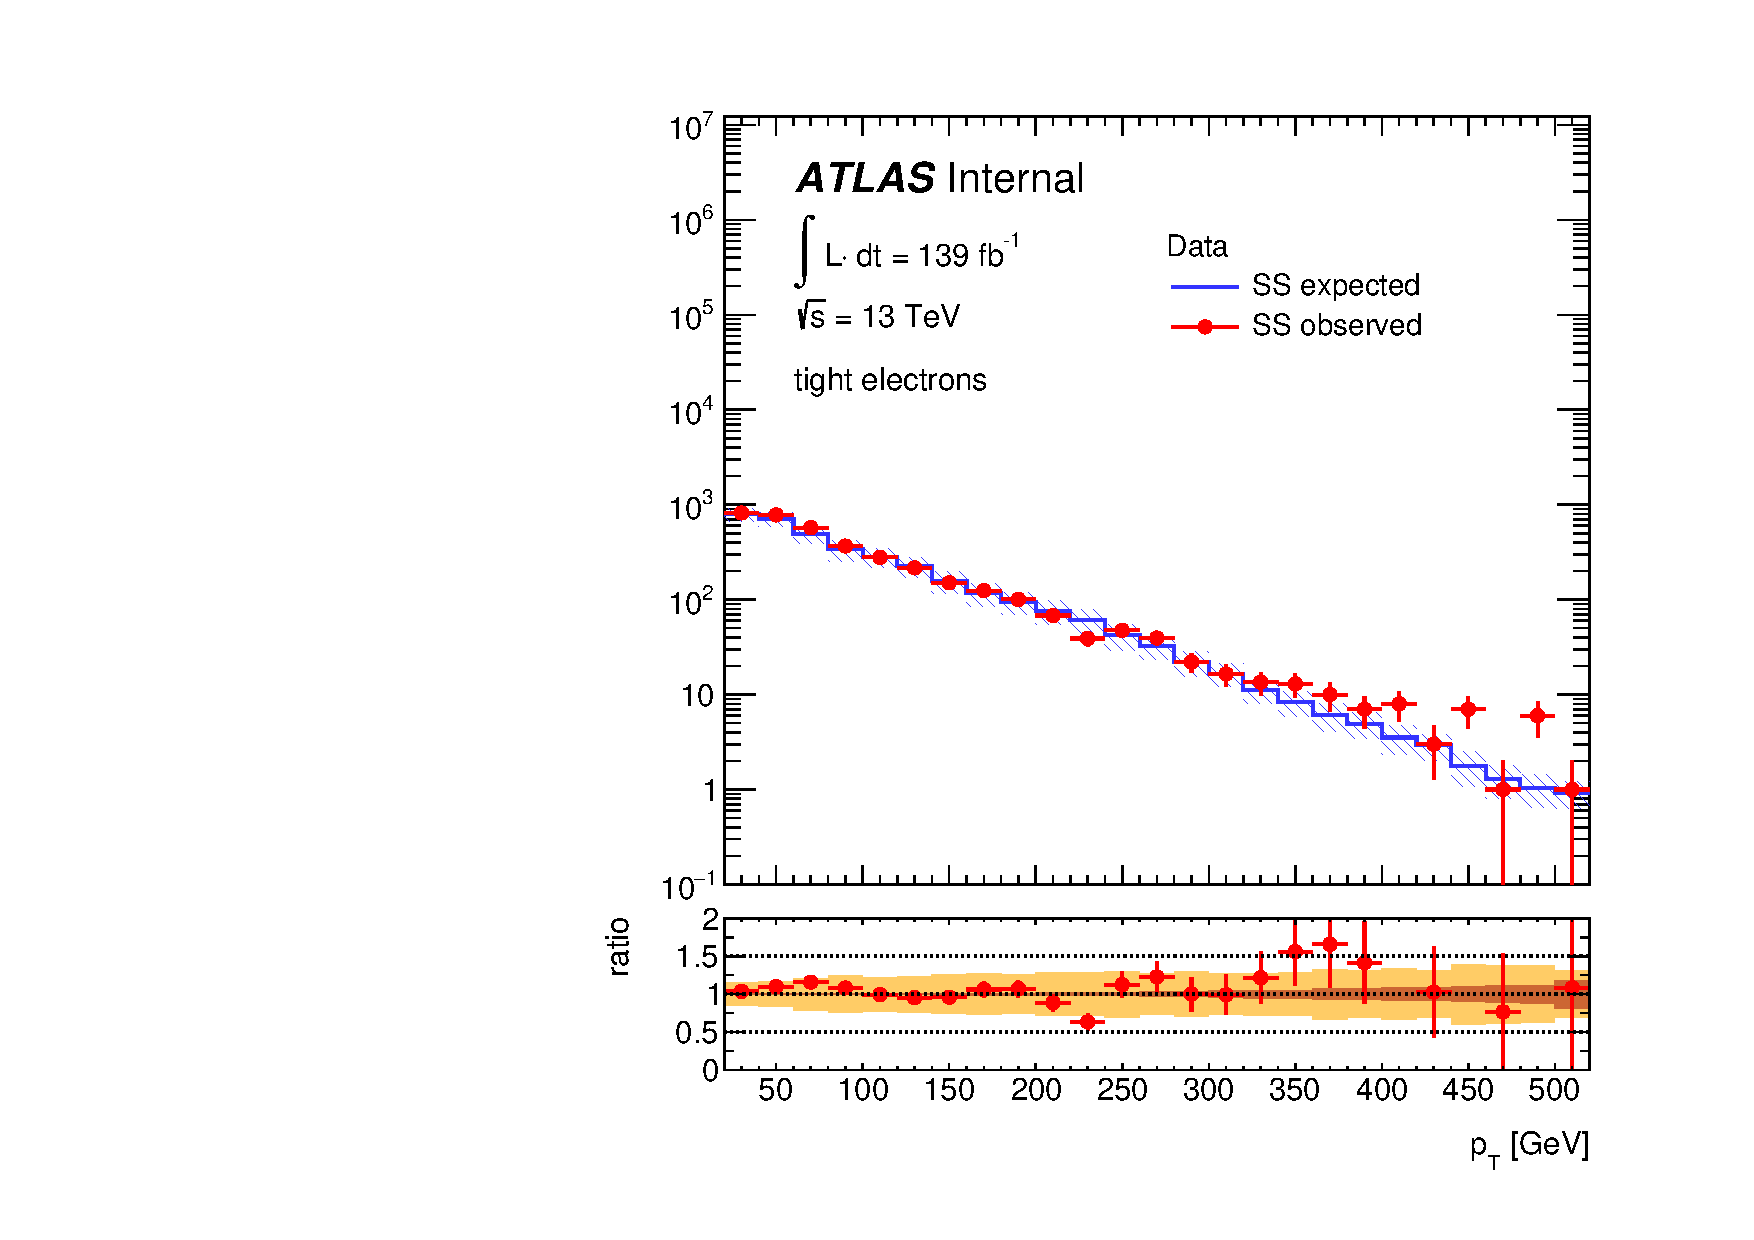
\includegraphics[width=0.45\textwidth]{figures/qmisid/valid_PttightData}\\
  \caption{Comparison between the expected and observed $\pT$ distribution of same-sign electrons.
  The dashed bands represent the total (statistical + systematic) uncertainty of the estimation. The comparison is shown for
  data events. The rates used to compute the predicted distribution are
  binned in $\pT$ (left) or continuous in $\pT$ (right).\label{fig:DatapTJumps}}
\end{figure}


\begin{figure}[tb!]
  \centering
  {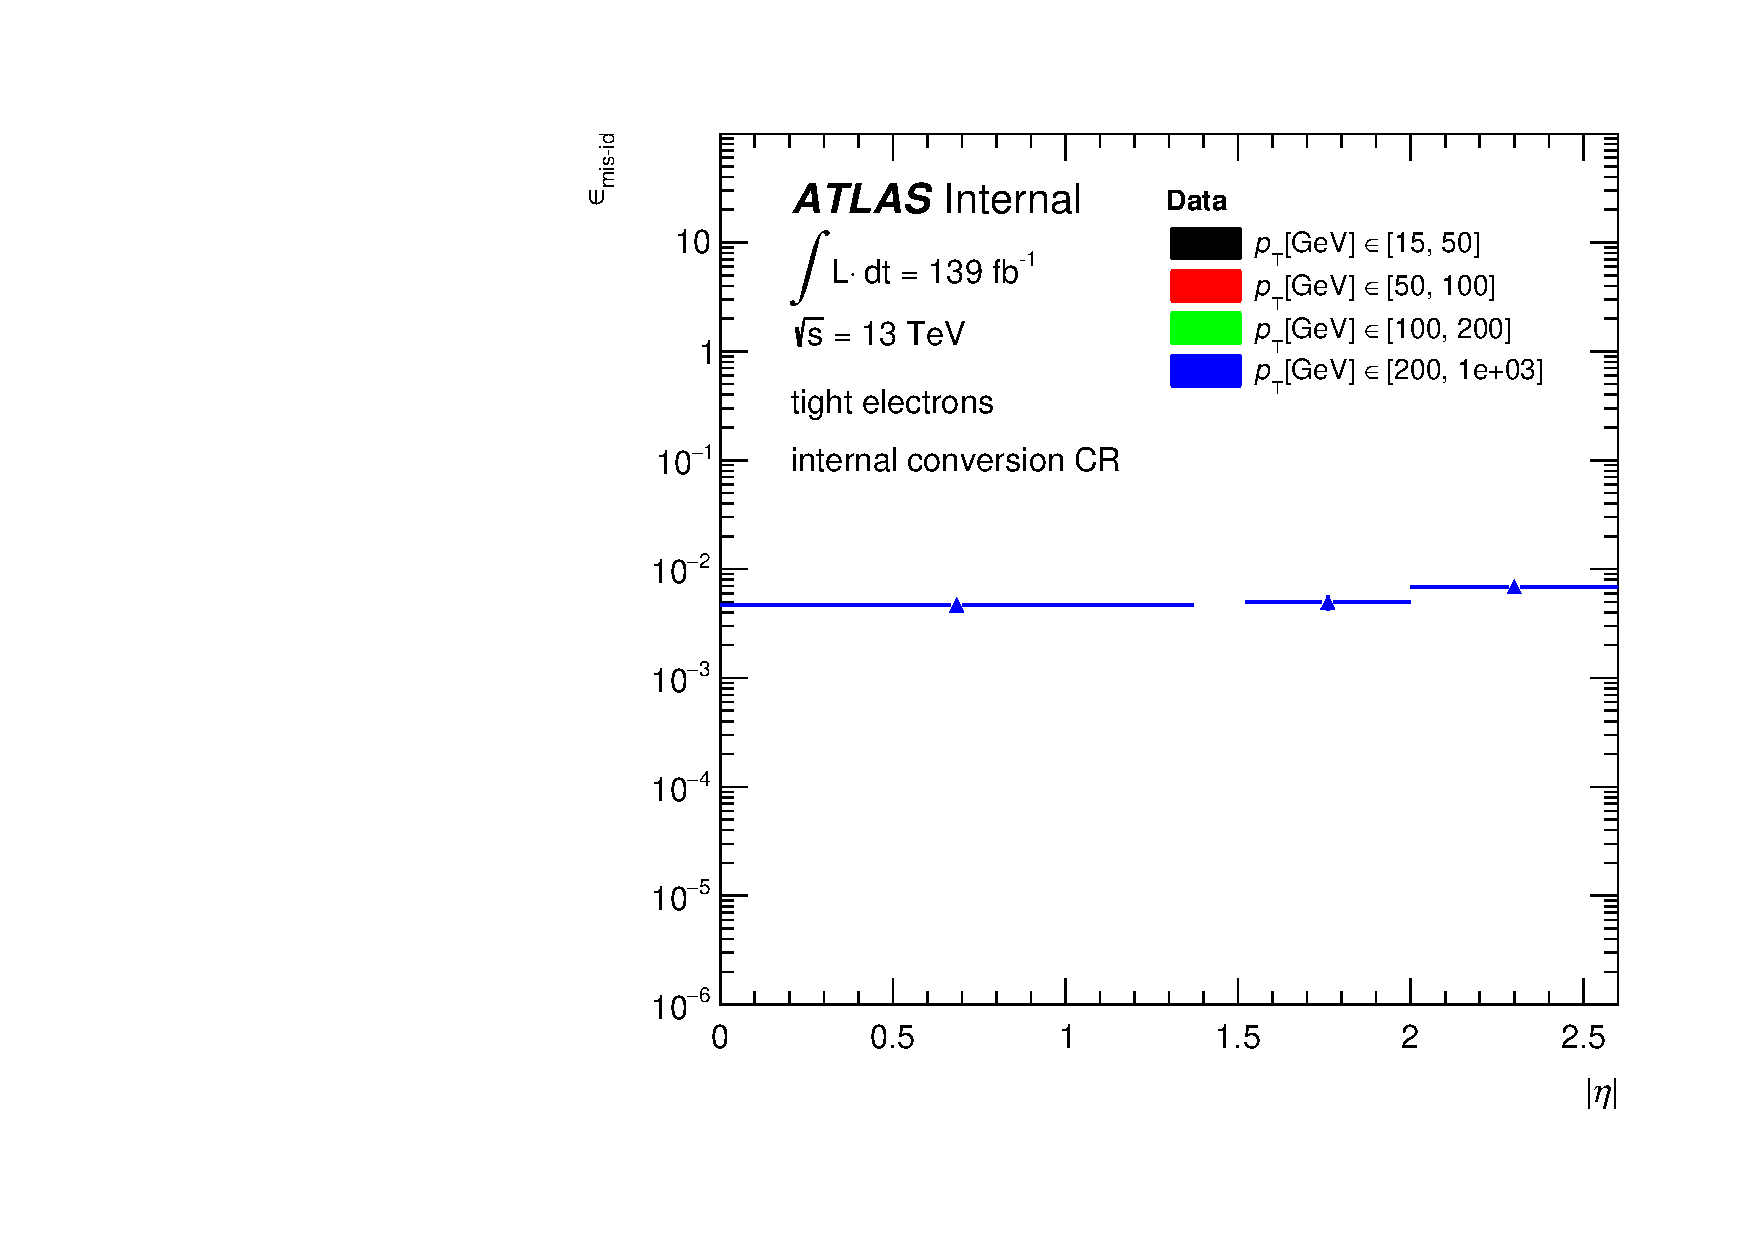
\includegraphics[width=0.37\textwidth]{figures/qmisid/crateData_tight_m0}}
  {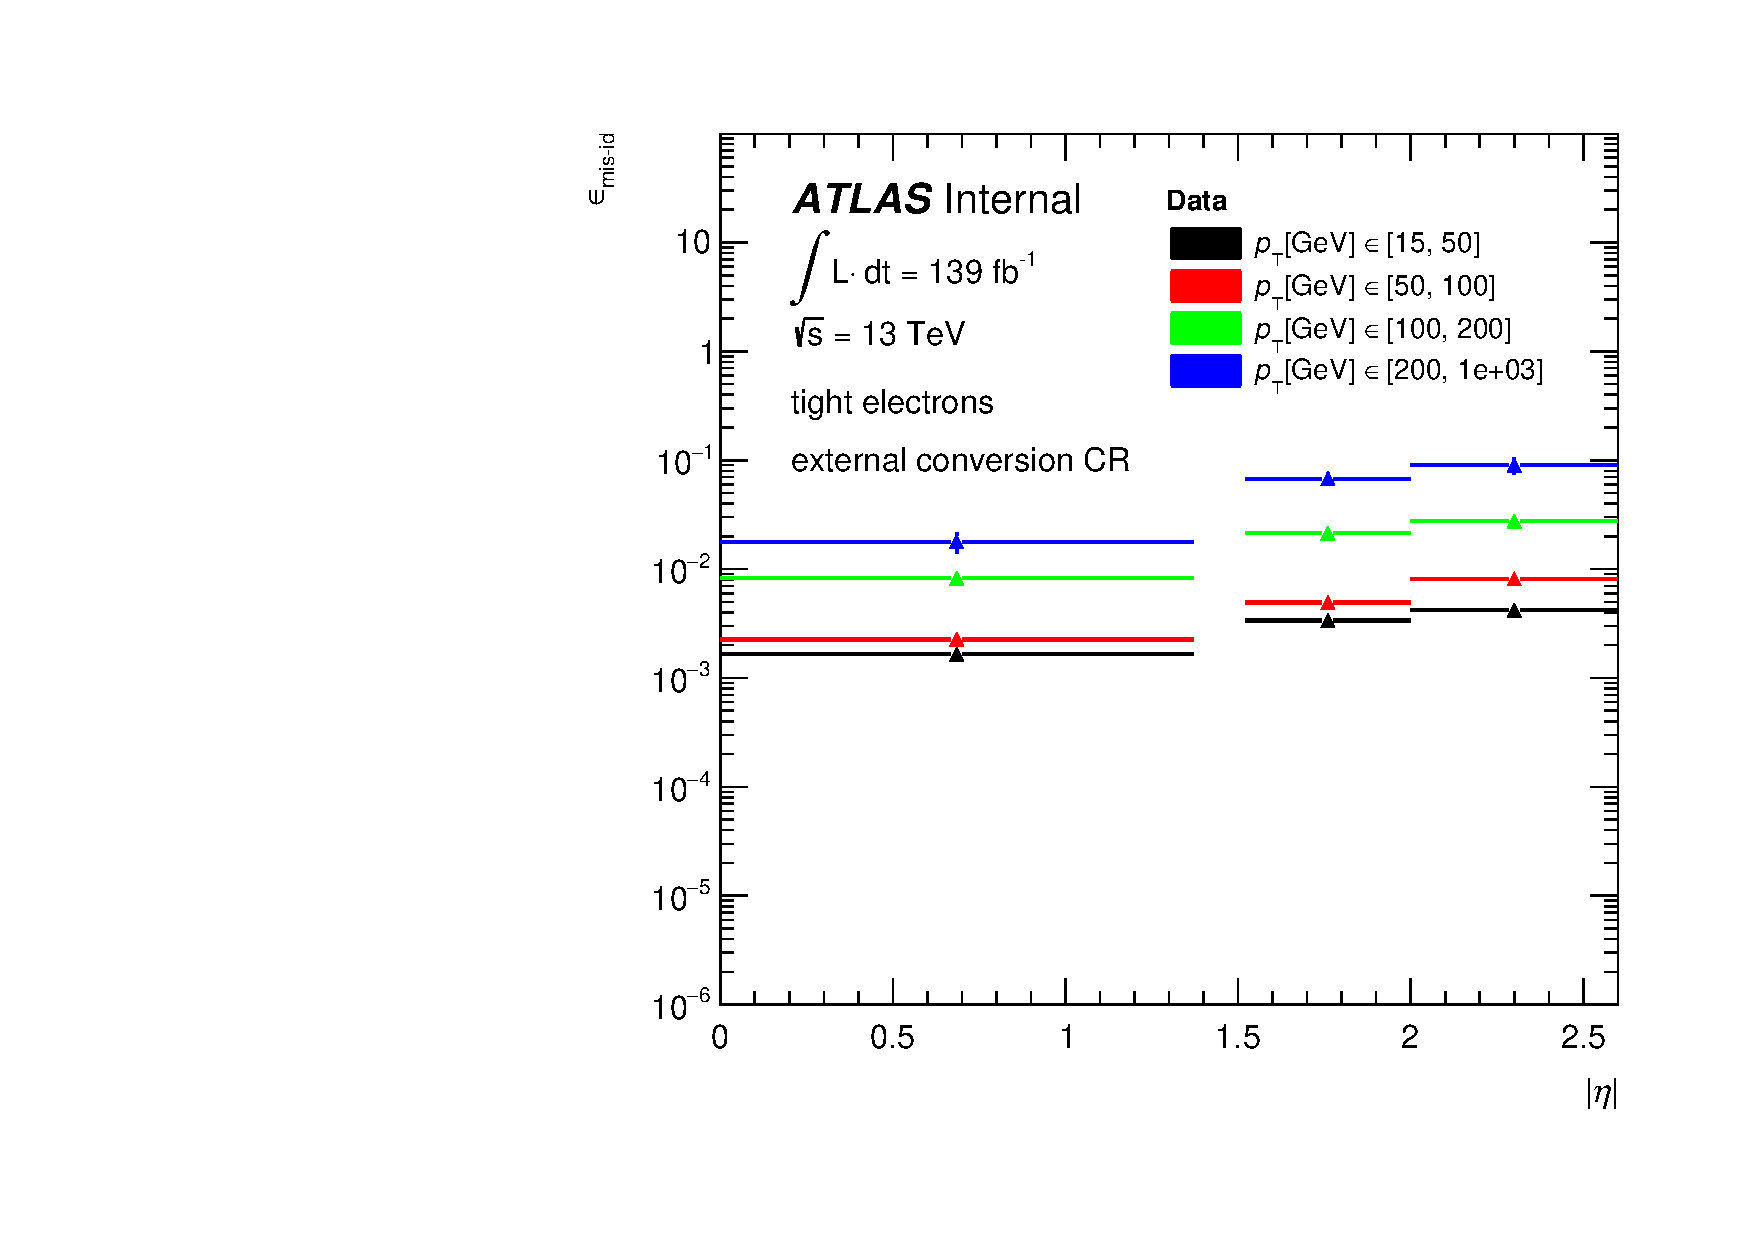
\includegraphics[width=0.37\textwidth]{figures/qmisid/crateData_tight_m1}}\\
  {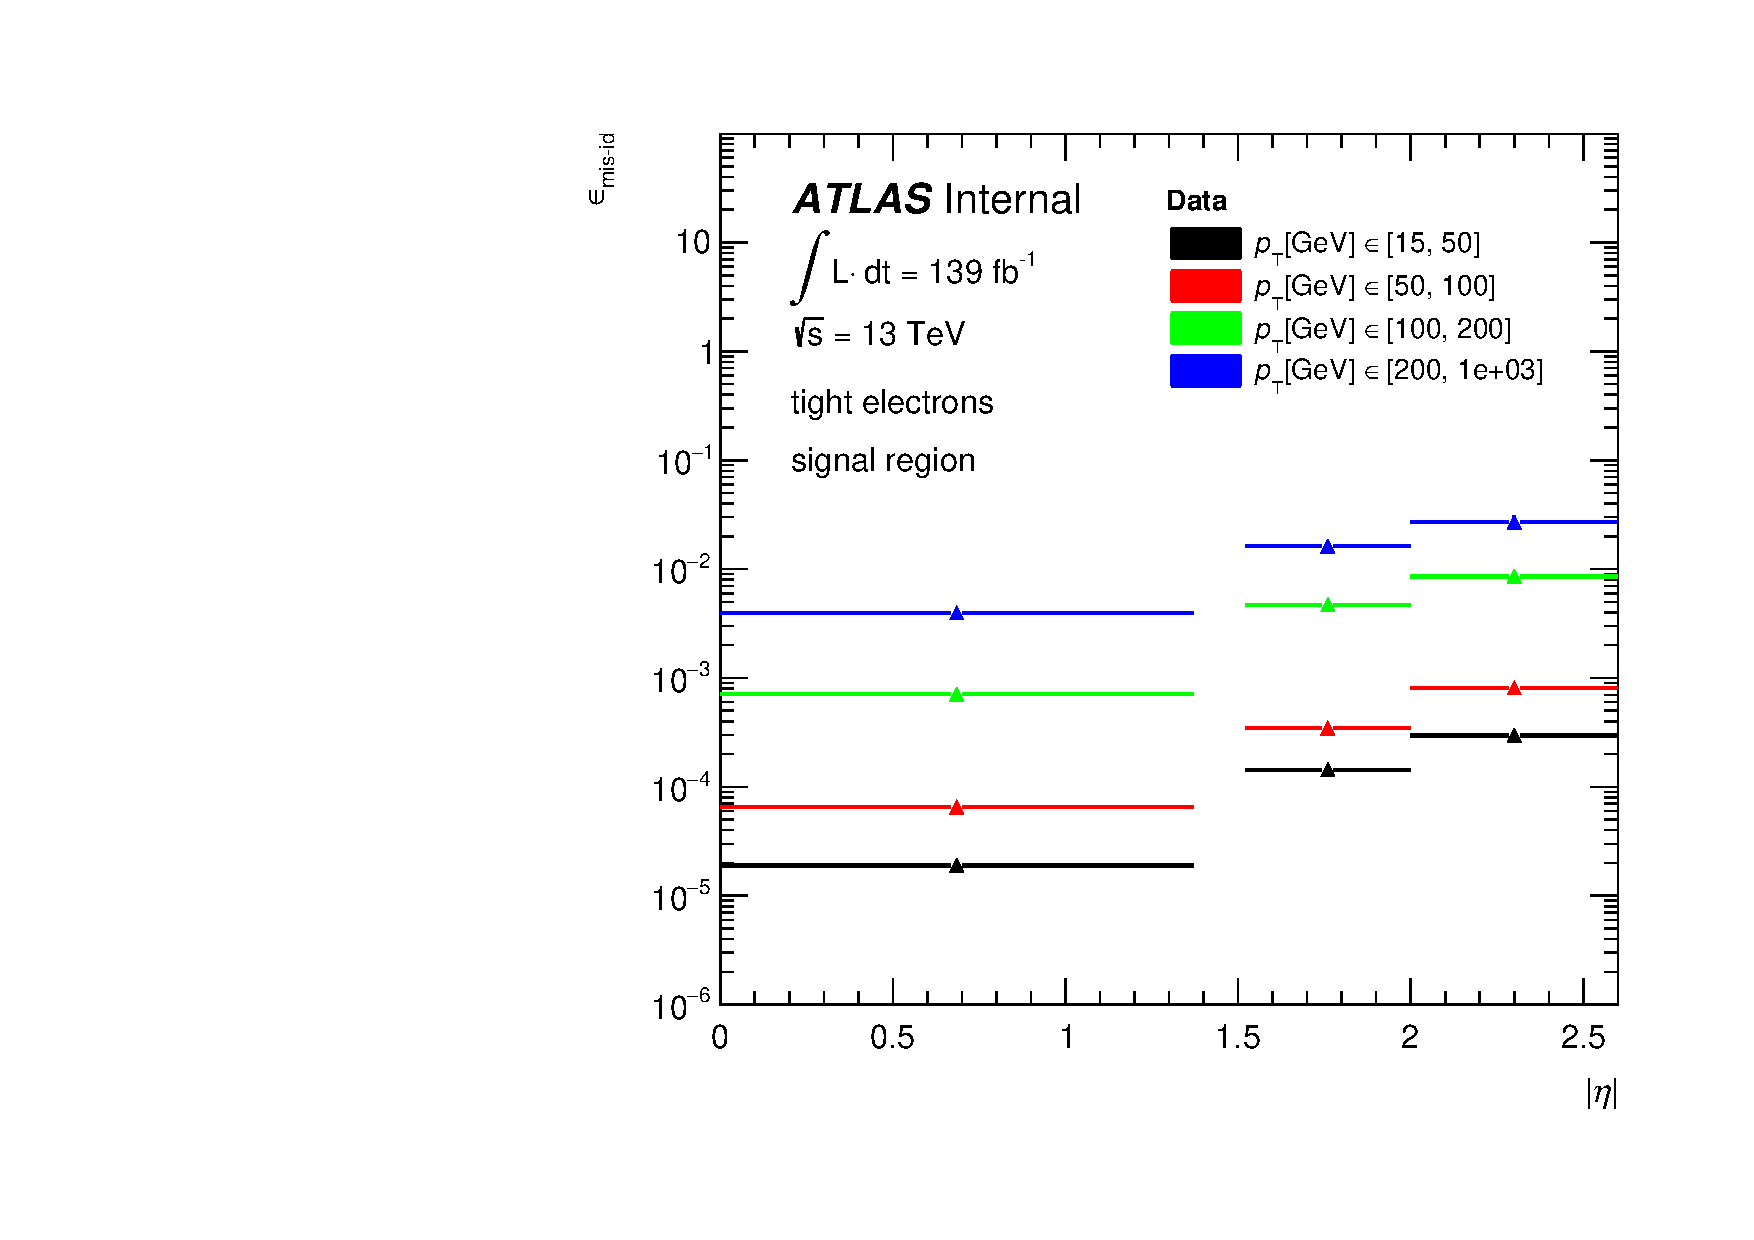
\includegraphics[width=0.37\textwidth]{figures/qmisid/crateData_tight_m2}}
  \caption{QMisID rates derived from the data with the likelihood method for tight electrons. 
           The rates are presented as a function of $|\eta|$ and parameterised in $\pT$ for the 
           photon-conversion CRs and the signal region. Due to lack of statistics, the
           the bins in $\pT$ are merged for the internal-conversion CR.\label{fig:Lik2Ddata}}
\end{figure}

%~~~~~~~~~~~~~~~~~~~~~~~~~~~~~~~~~~~~~~~~~~~~~~~~~~~~~~~~~~~~~~~
\subsubsection{Validation of the likelihood method (truth-closure)}
%~~~~~~~~~~~~~~~~~~~~~~~~~~~~~~~~~~~~~~~~~~~~~~~~~~~~~~~~~~~~~~~

To validate the likelihood method the QMisID rates are derived from simulated $Z$+jets events and compared to the 
rates based on the MC truth information (truth-matching). The comparison is shown in figure\,\ref{fig:LikTruthT} 
as a function of $|\eta|$ and parameterised in $\pT$. To mitigate the large statistical uncertainties introduced due 
to the size of the MC sample, the $|\eta|$-bins are merged. Furthermore, for the internal conversion region, $\pT$ 
bins are also merged. The results show no significant disagreement between the two approaches. Any difference is 
considered as a systematic uncertainty to the rates (see section\,\ref{Sec:systematic}). Finally, the same comparison 
is presented for the case of anti-tight electrons in order to verity the agreement of the two approaches with 
higher statistics.  

\begin{figure}[tb!]
  \centering
  {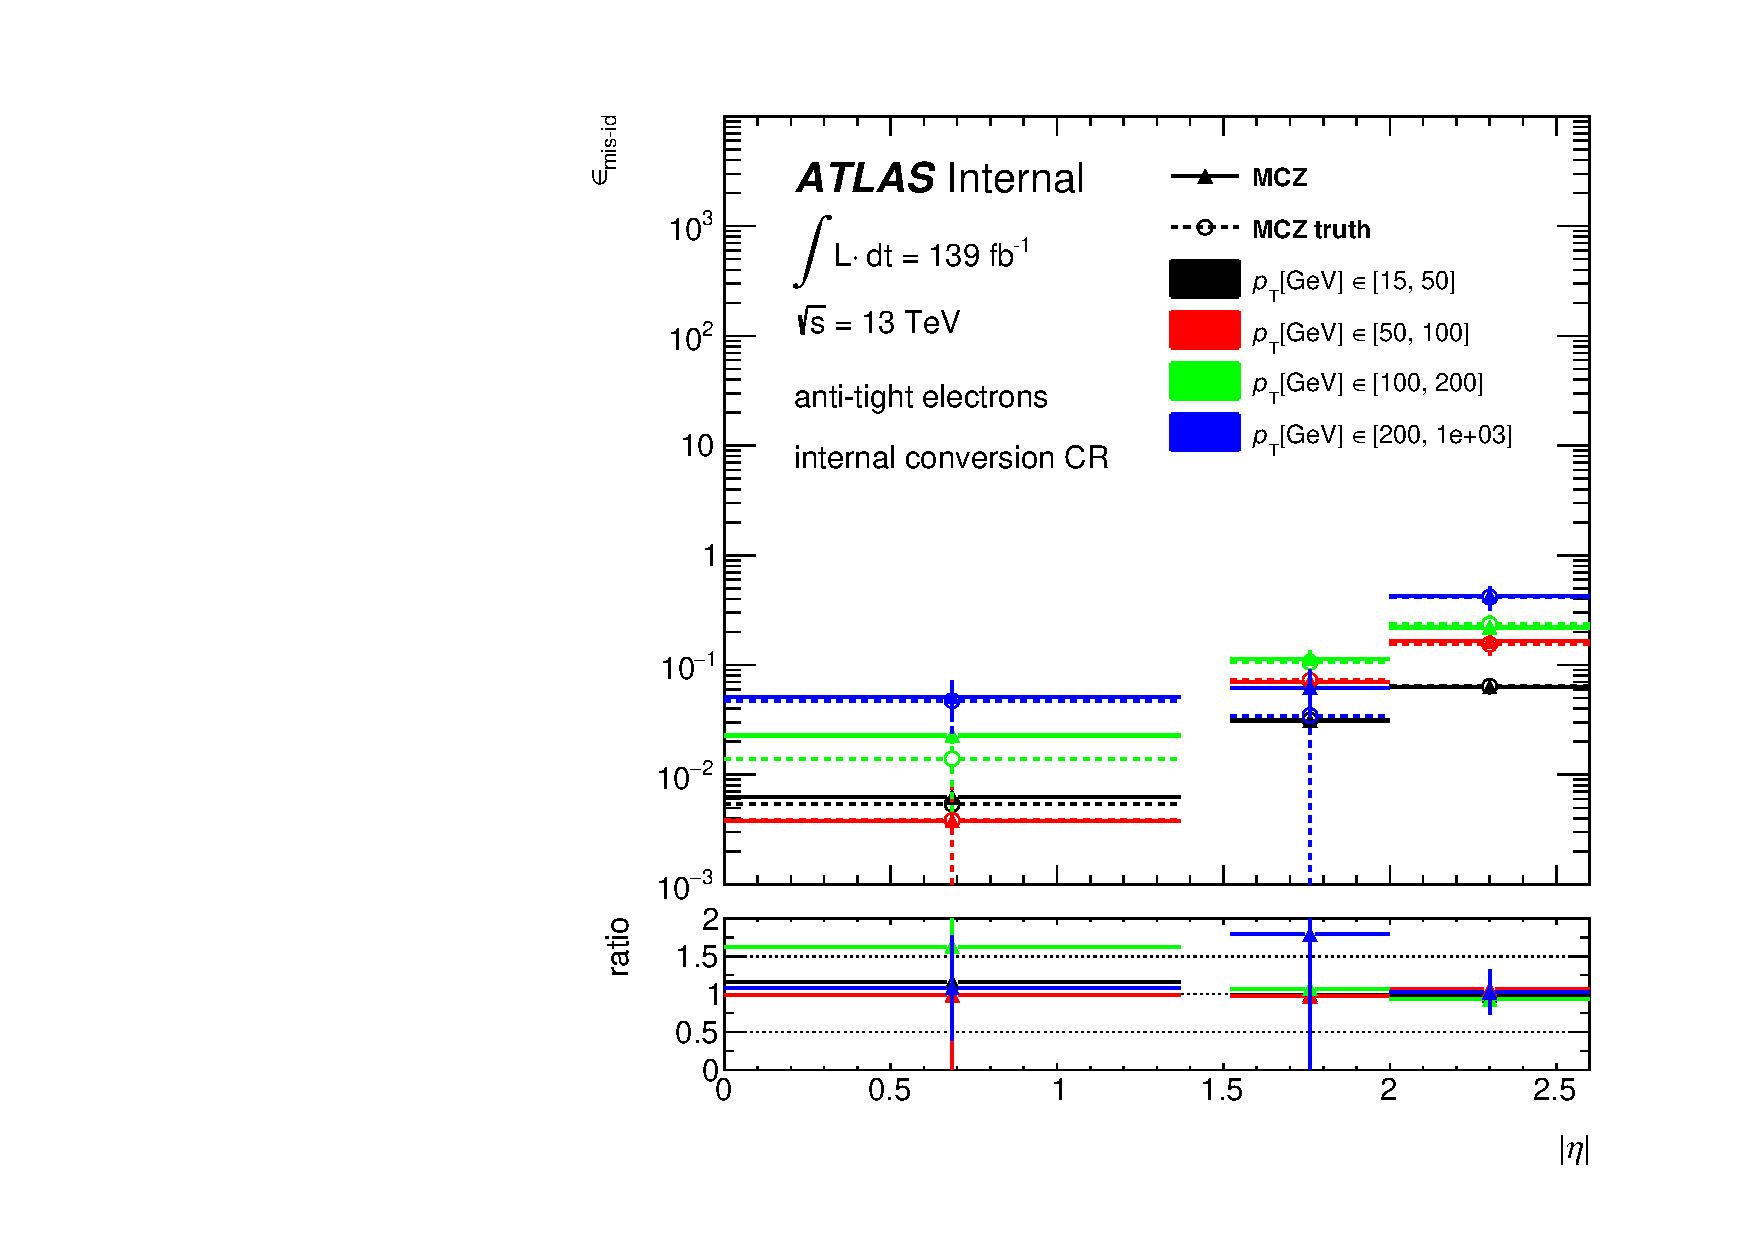
\includegraphics[width=0.45\textwidth]{figures/qmisid/crateMCZ_MCZtruth_atight_m0}}
  {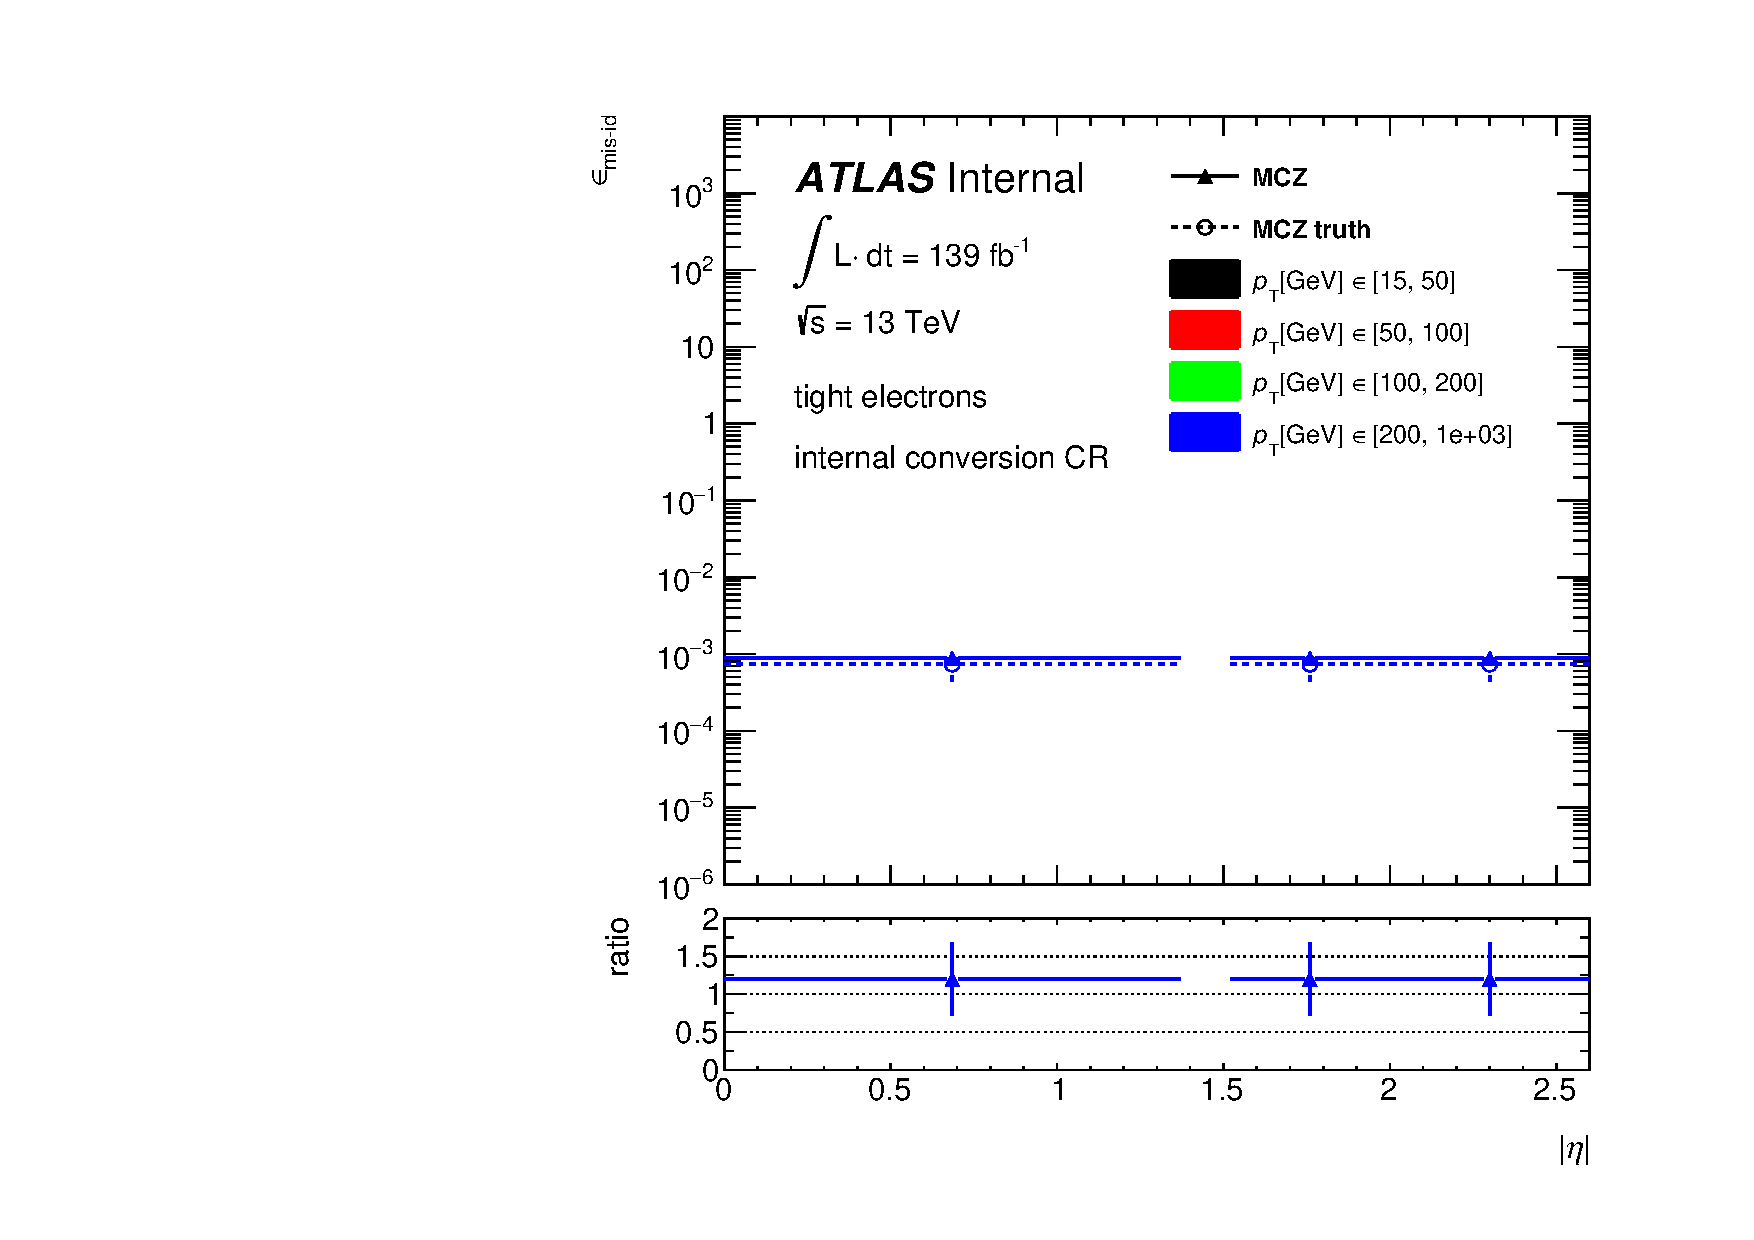
\includegraphics[width=0.45\textwidth]{figures/qmisid/crateMCZ_MCZtruth_tight_m0}}\\
  {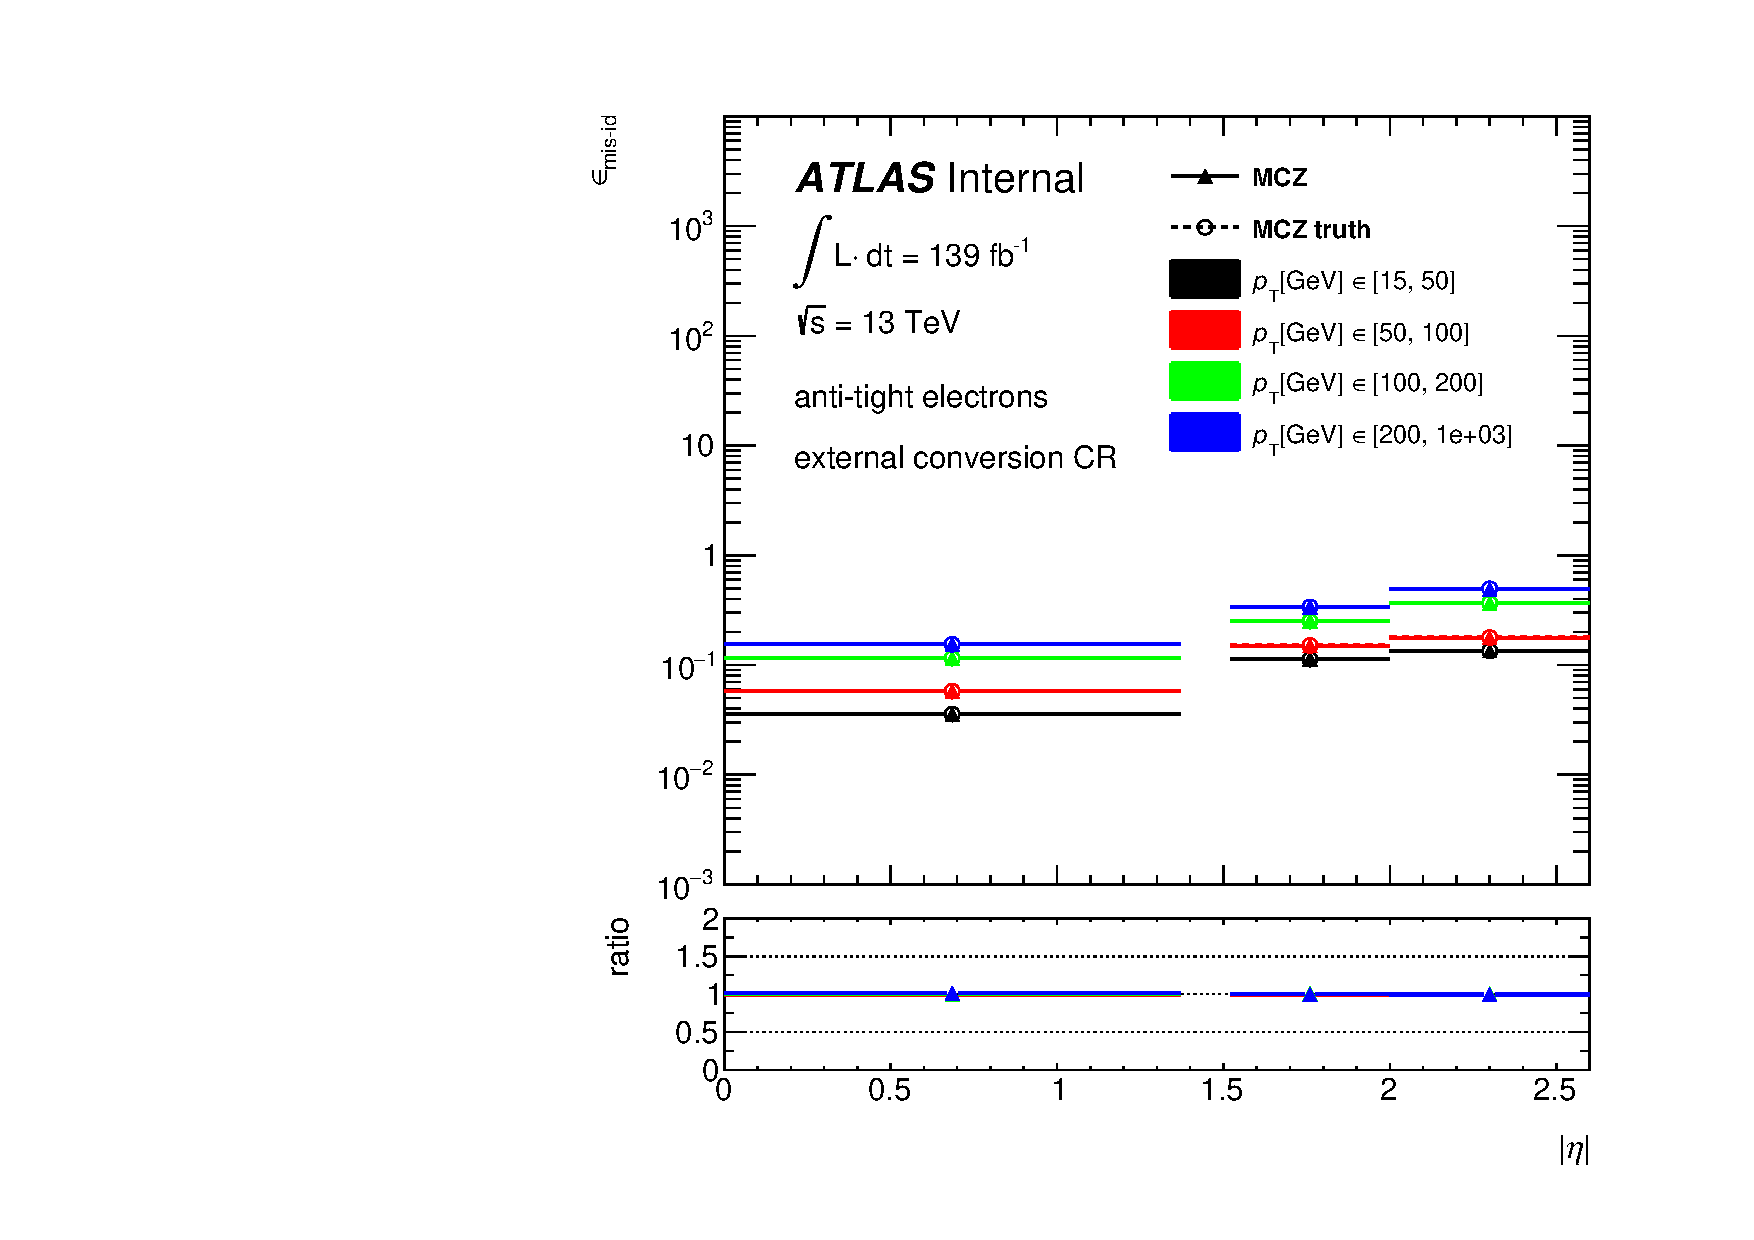
\includegraphics[width=0.45\textwidth]{figures/qmisid/crateMCZ_MCZtruth_atight_m1}}
  {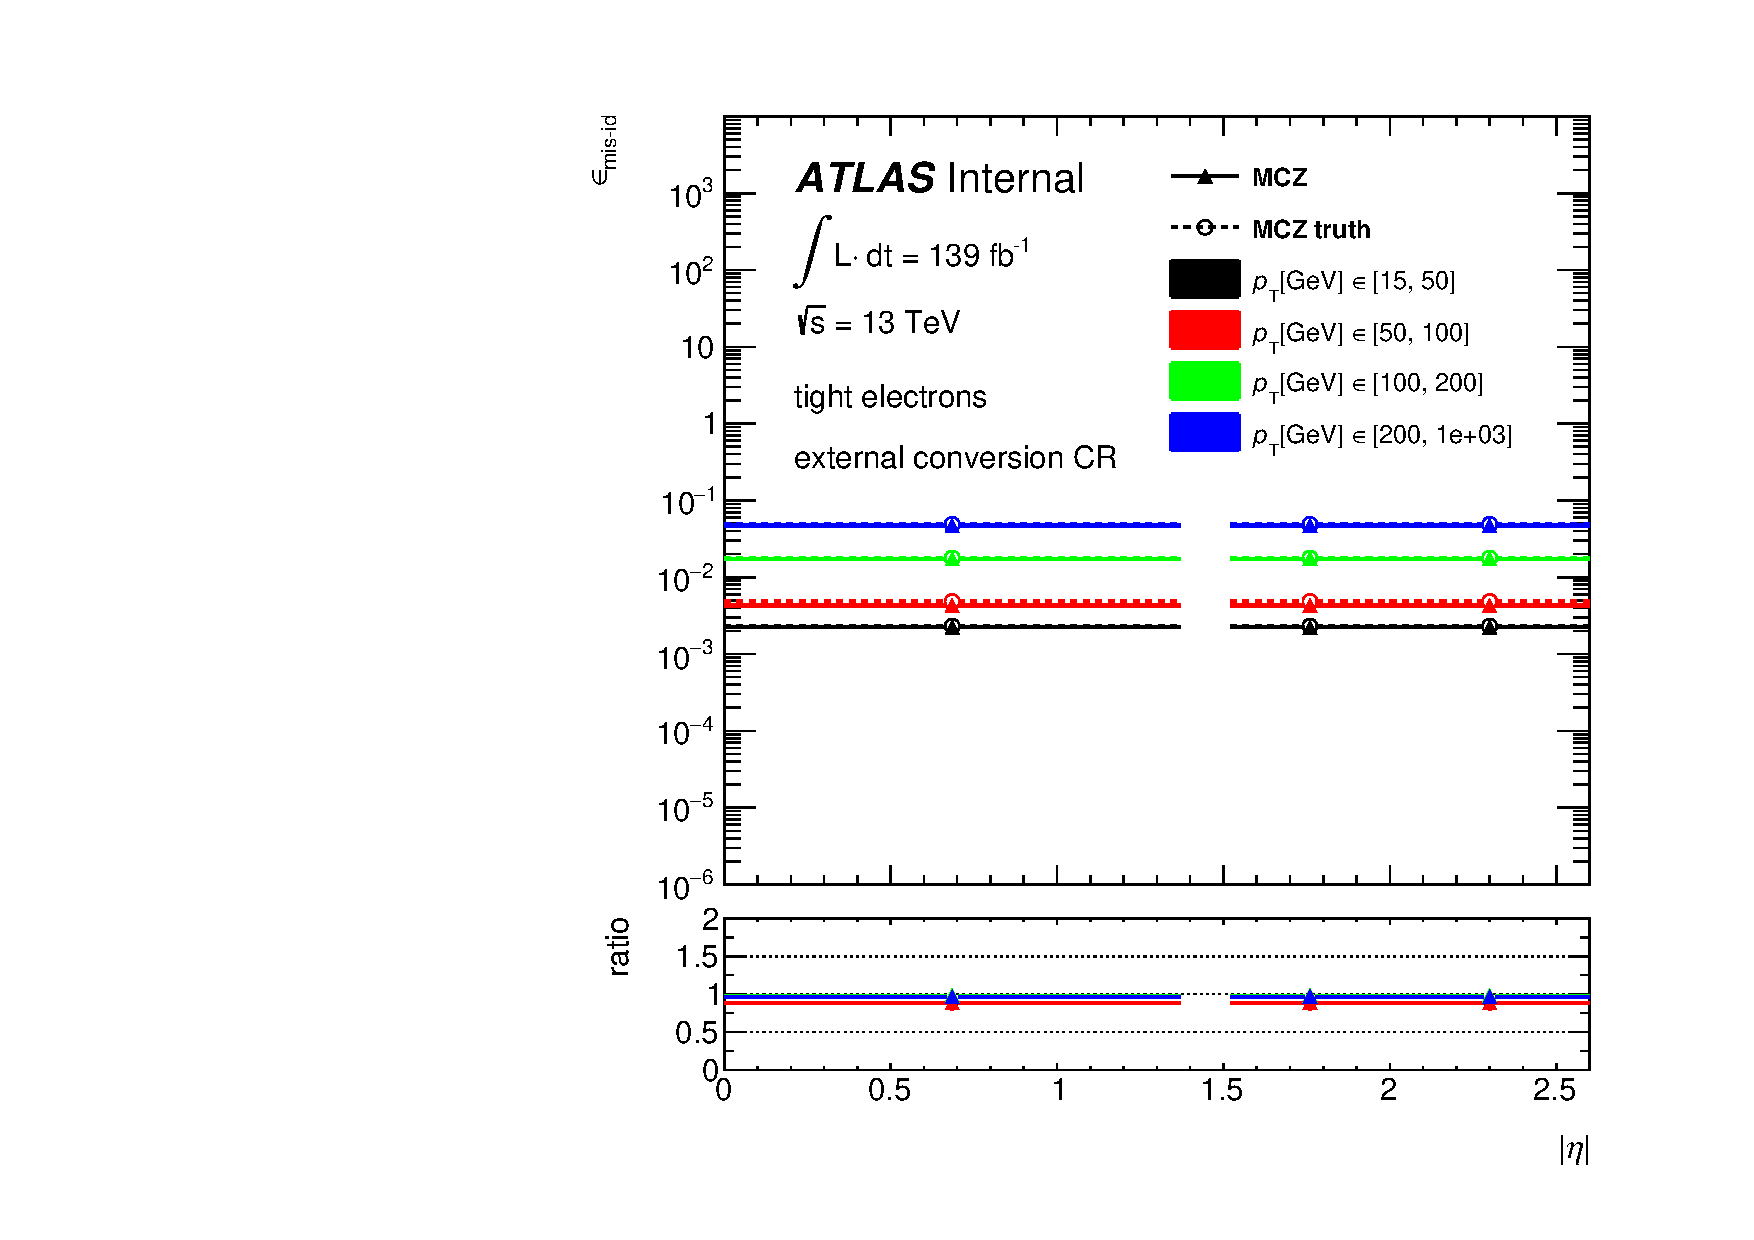
\includegraphics[width=0.45\textwidth]{figures/qmisid/crateMCZ_MCZtruth_tight_m1}}\\
  {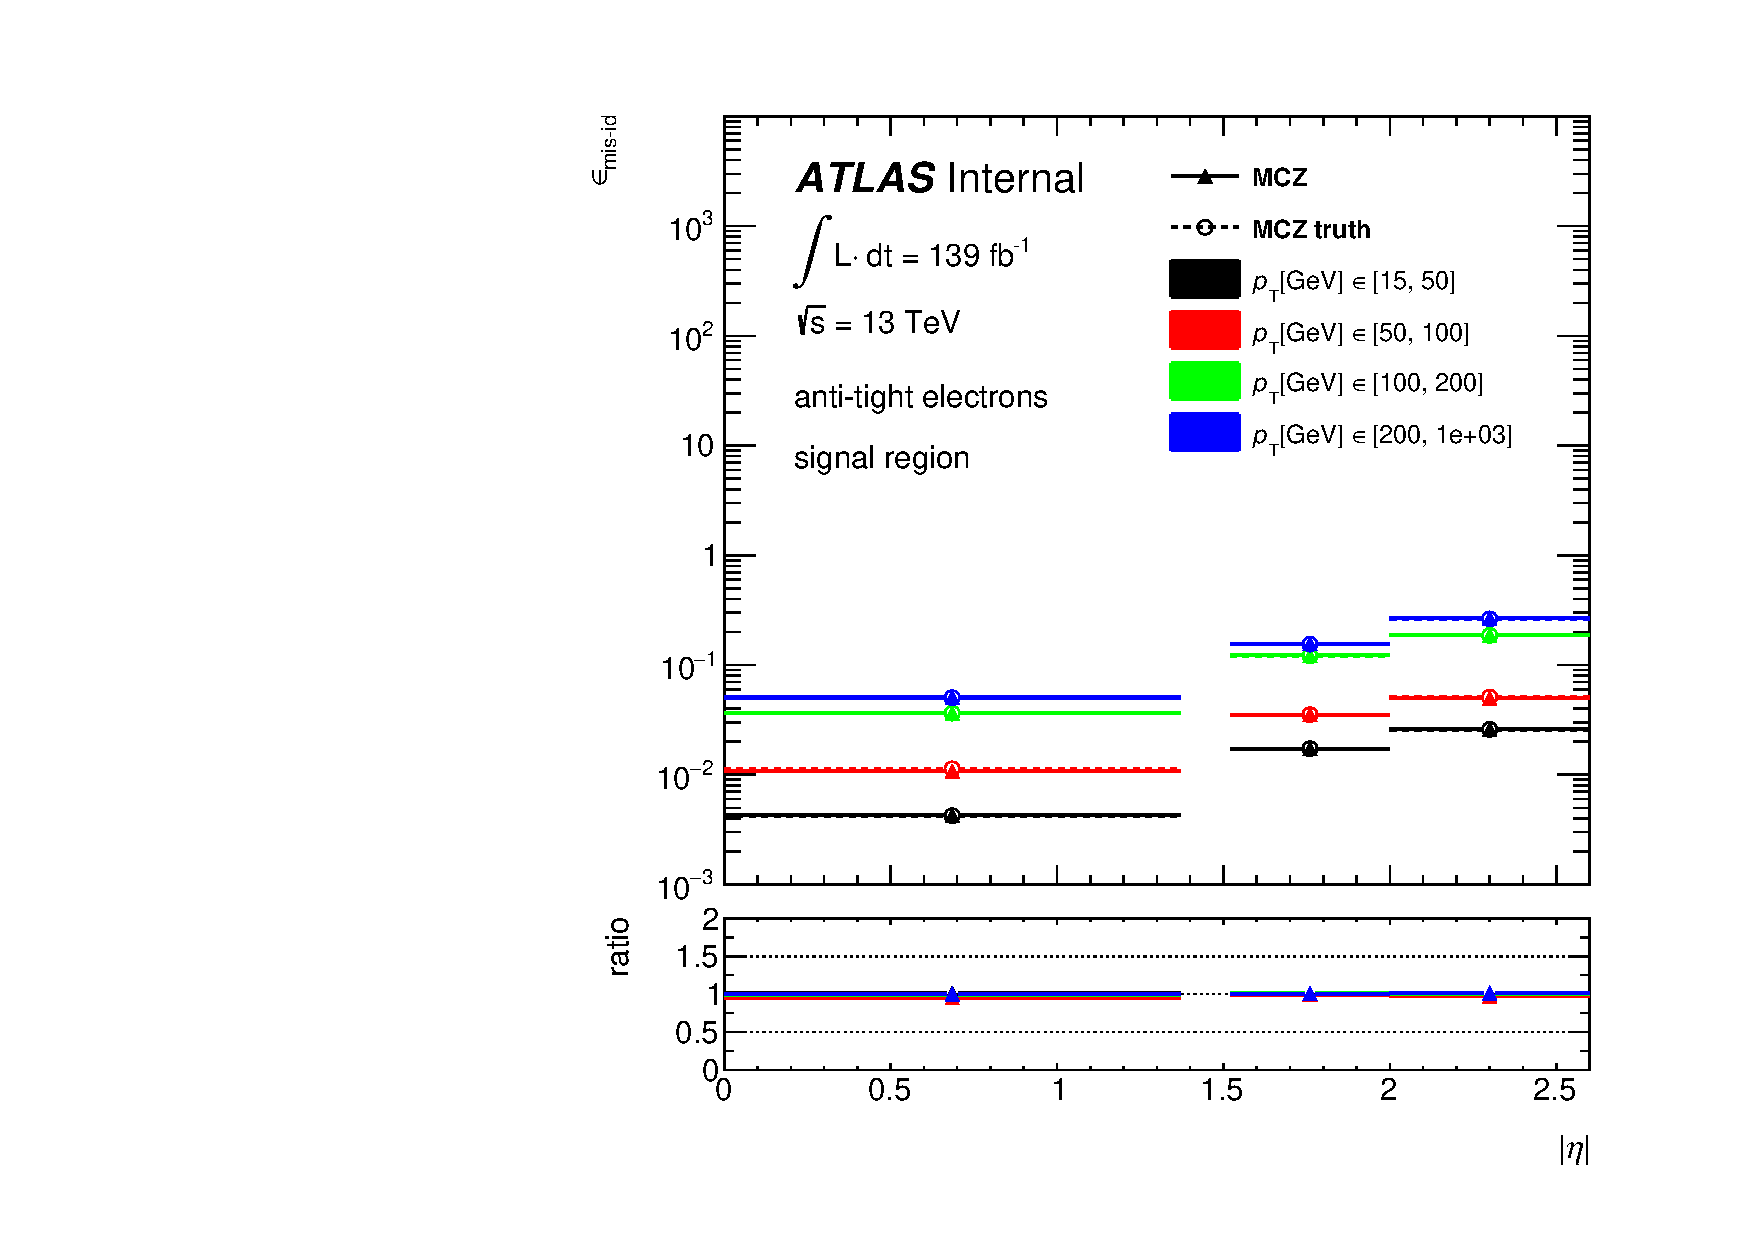
\includegraphics[width=0.45\textwidth]{figures/qmisid/crateMCZ_MCZtruth_atight_m2}}
  {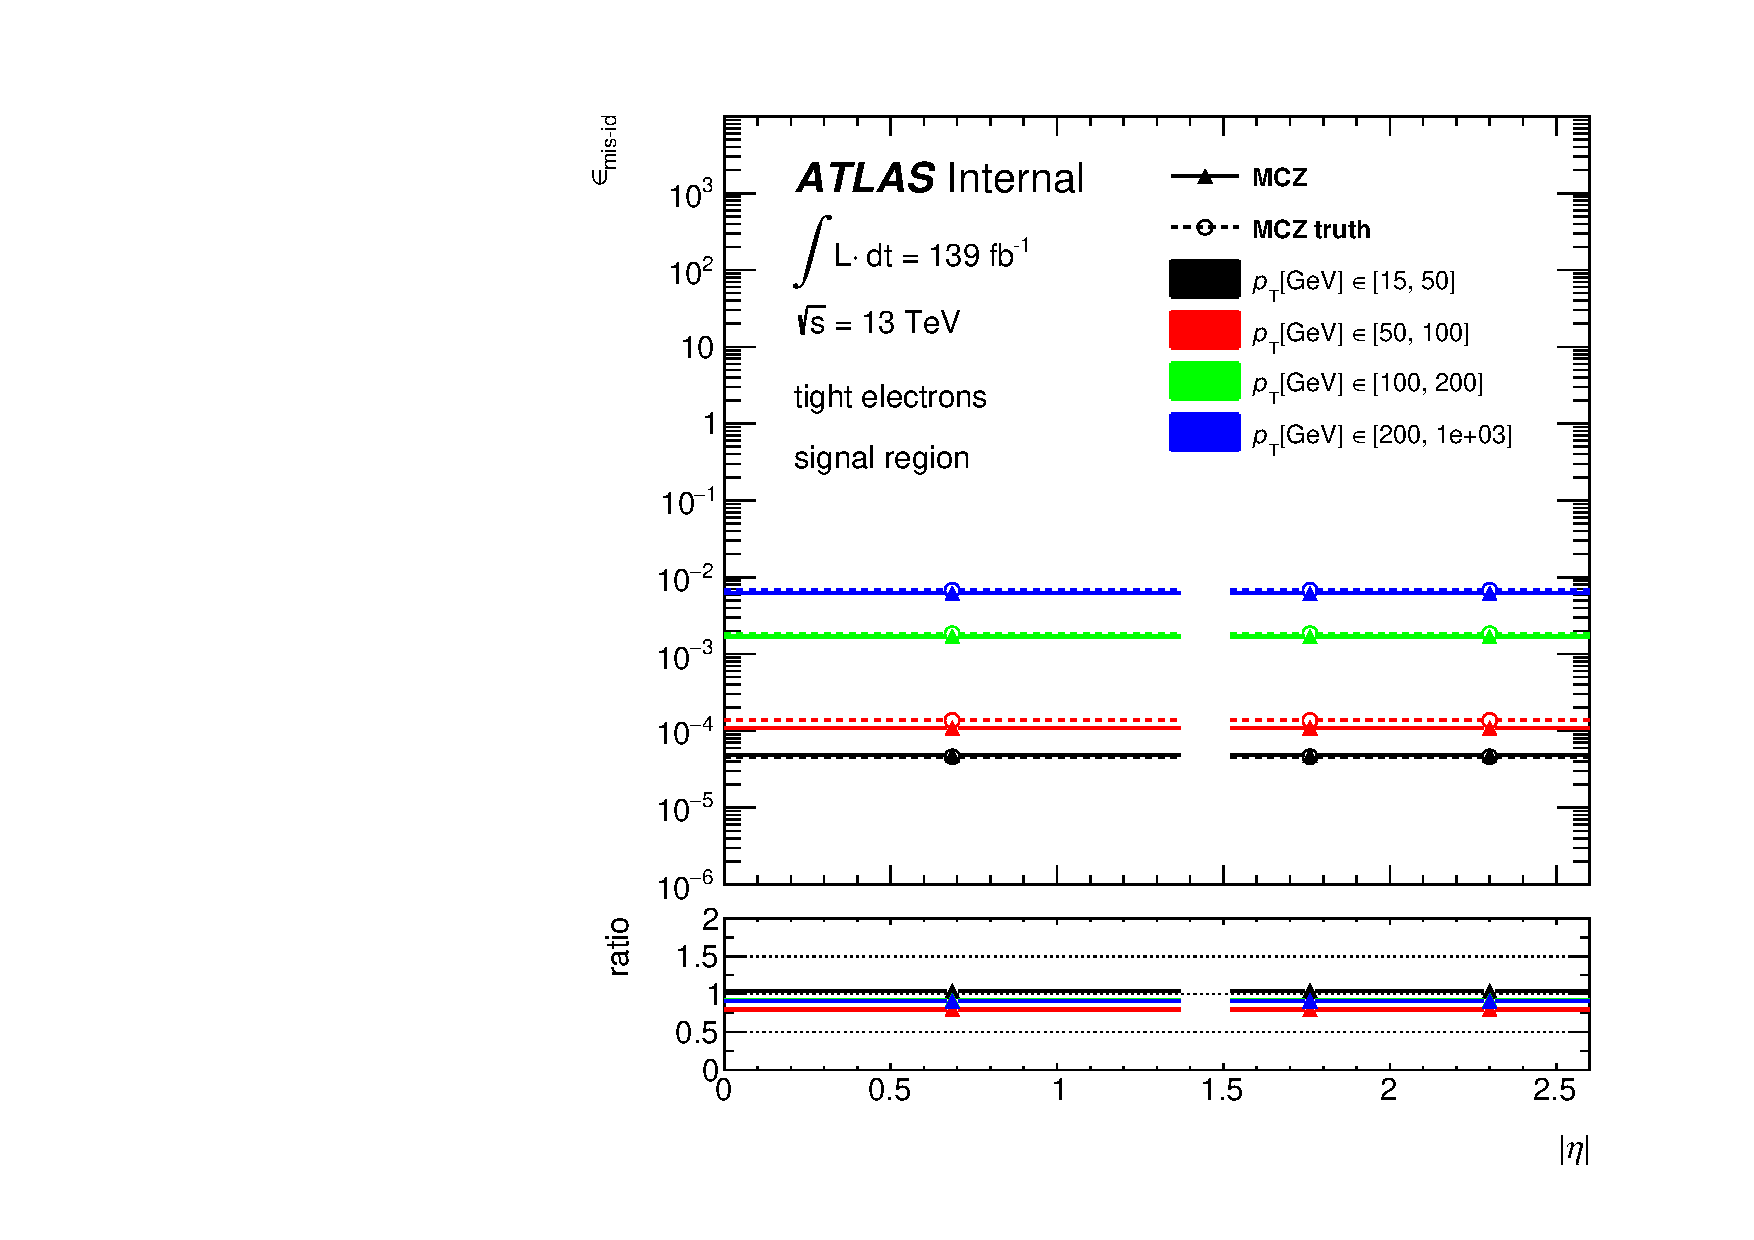
\includegraphics[width=0.45\textwidth]{figures/qmisid/crateMCZ_MCZtruth_tight_m2}}
  \caption{QMisID rates derived from $Z\rightarrow ee$ simulated events with the likelihood method, compared to truth-based
           rates for anti-tight (left) and tight (right) electrons. The rates are presented as a function of $|\eta|$,
           parameterised in $\pT$ for the photon-conversion CRs and the signal region. Due to lack of statistics, in 
           the case of tight electrons, the bins in $|\eta|$ are merged. For the internal-conversion CR, the bins in 
           $\pT$ are also merged.\label{fig:LikTruthT}}
\end{figure}

\clearpage

%~~~~~~~~~~~~~~~~~~~~~~~~~~~~~~~~~~~
\subsubsection{Systematic uncertainties}
\label{Sec:systematic}
%~~~~~~~~~~~~~~~~~~~~~~~~~~~~~~~~~~~

Four sources of systematic uncertainties are assigned to the QMisiD rates:

\begin{itemize}
\item the error estimates from the likelihood maximisation (figure\,\ref{fig:QMisID:systa}) which depend on the 
      statistical size of the control region of the data in which the rates are estimated;
\item the difference between the rates measured with the likelihood method and those obtained by truth-matching 
      with simulated $Z\rightarrow ee$ events (figure\,\ref{fig:QMisID:systa});
\item the variation of the rates with the $m_Z$ window
  (figure\,\ref{fig:QMisID:systb});
\item low $m_{ee}$ mismodelings observed on simulated $t\bar{t}$ samples and
  that can be relevant to some control regions.
\end{itemize}

The total uncertainty is defined as the quadratic sum of the above contributions (figure\,\ref{fig:QMisID:systb}).

\begin{figure}[p!]
  \begin{center}
  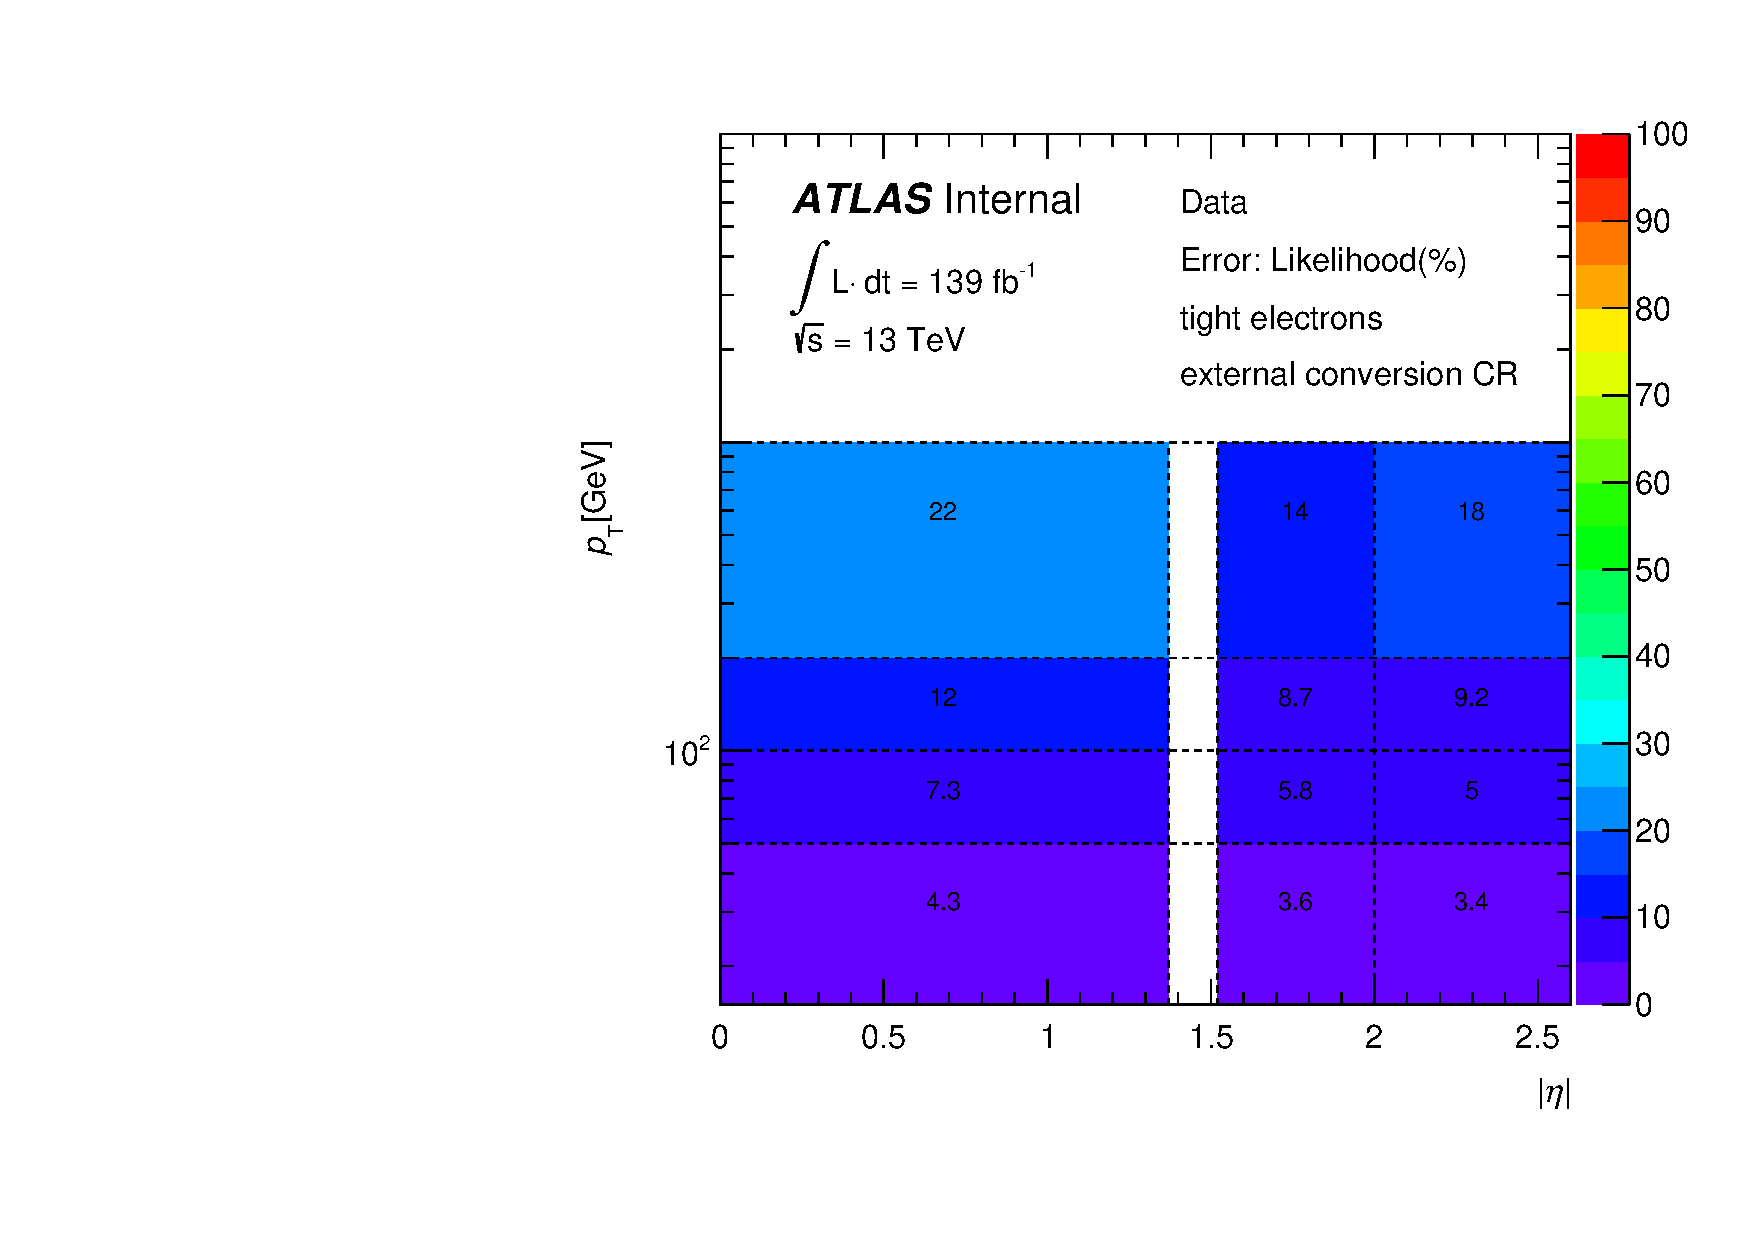
\includegraphics[width=0.45\textwidth]{figures/qmisid/syst_Data_Likelihood_tight_extcr}
  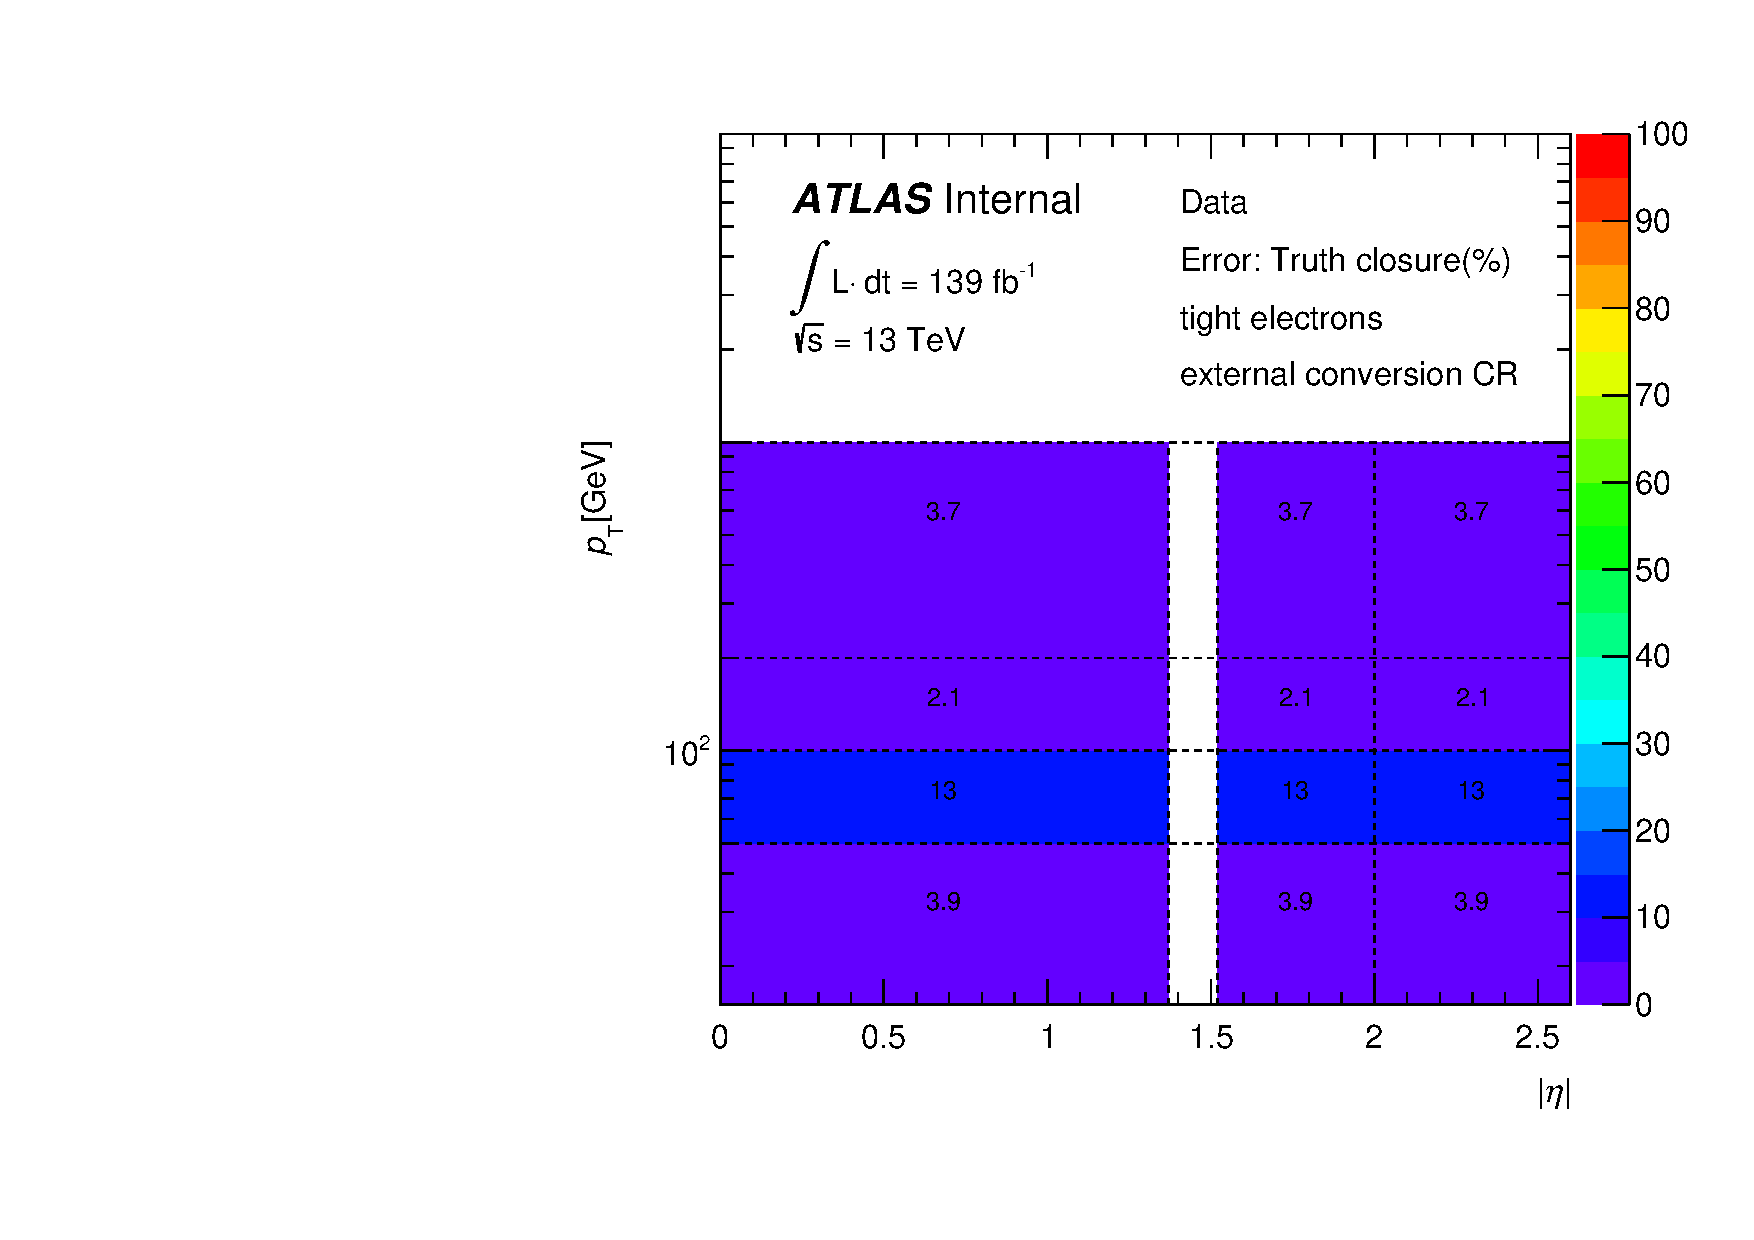
\includegraphics[width=0.45\textwidth]{figures/qmisid/syst_Data_Truthclosure_tight_extcr}\\
  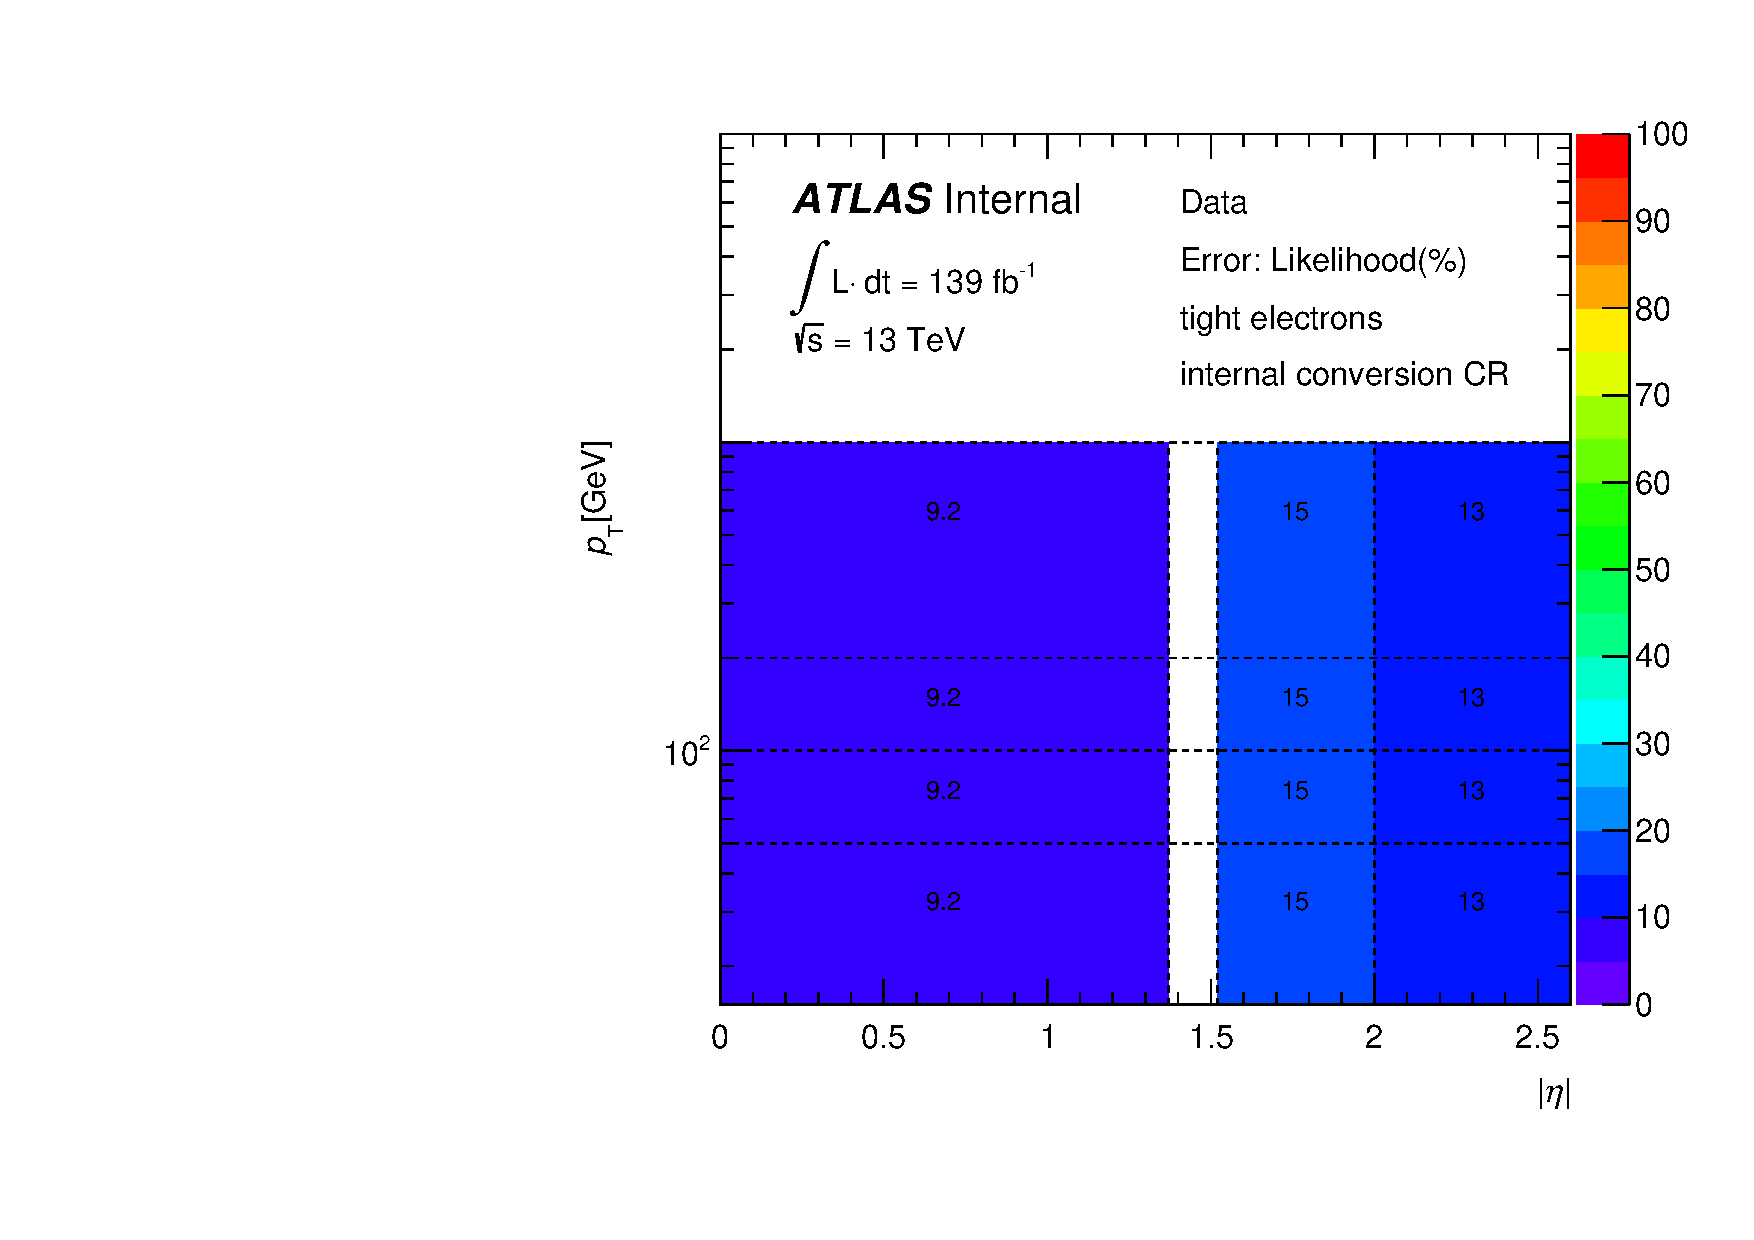
\includegraphics[width=0.45\textwidth]{figures/qmisid/syst_Data_Likelihood_tight_intcr}
  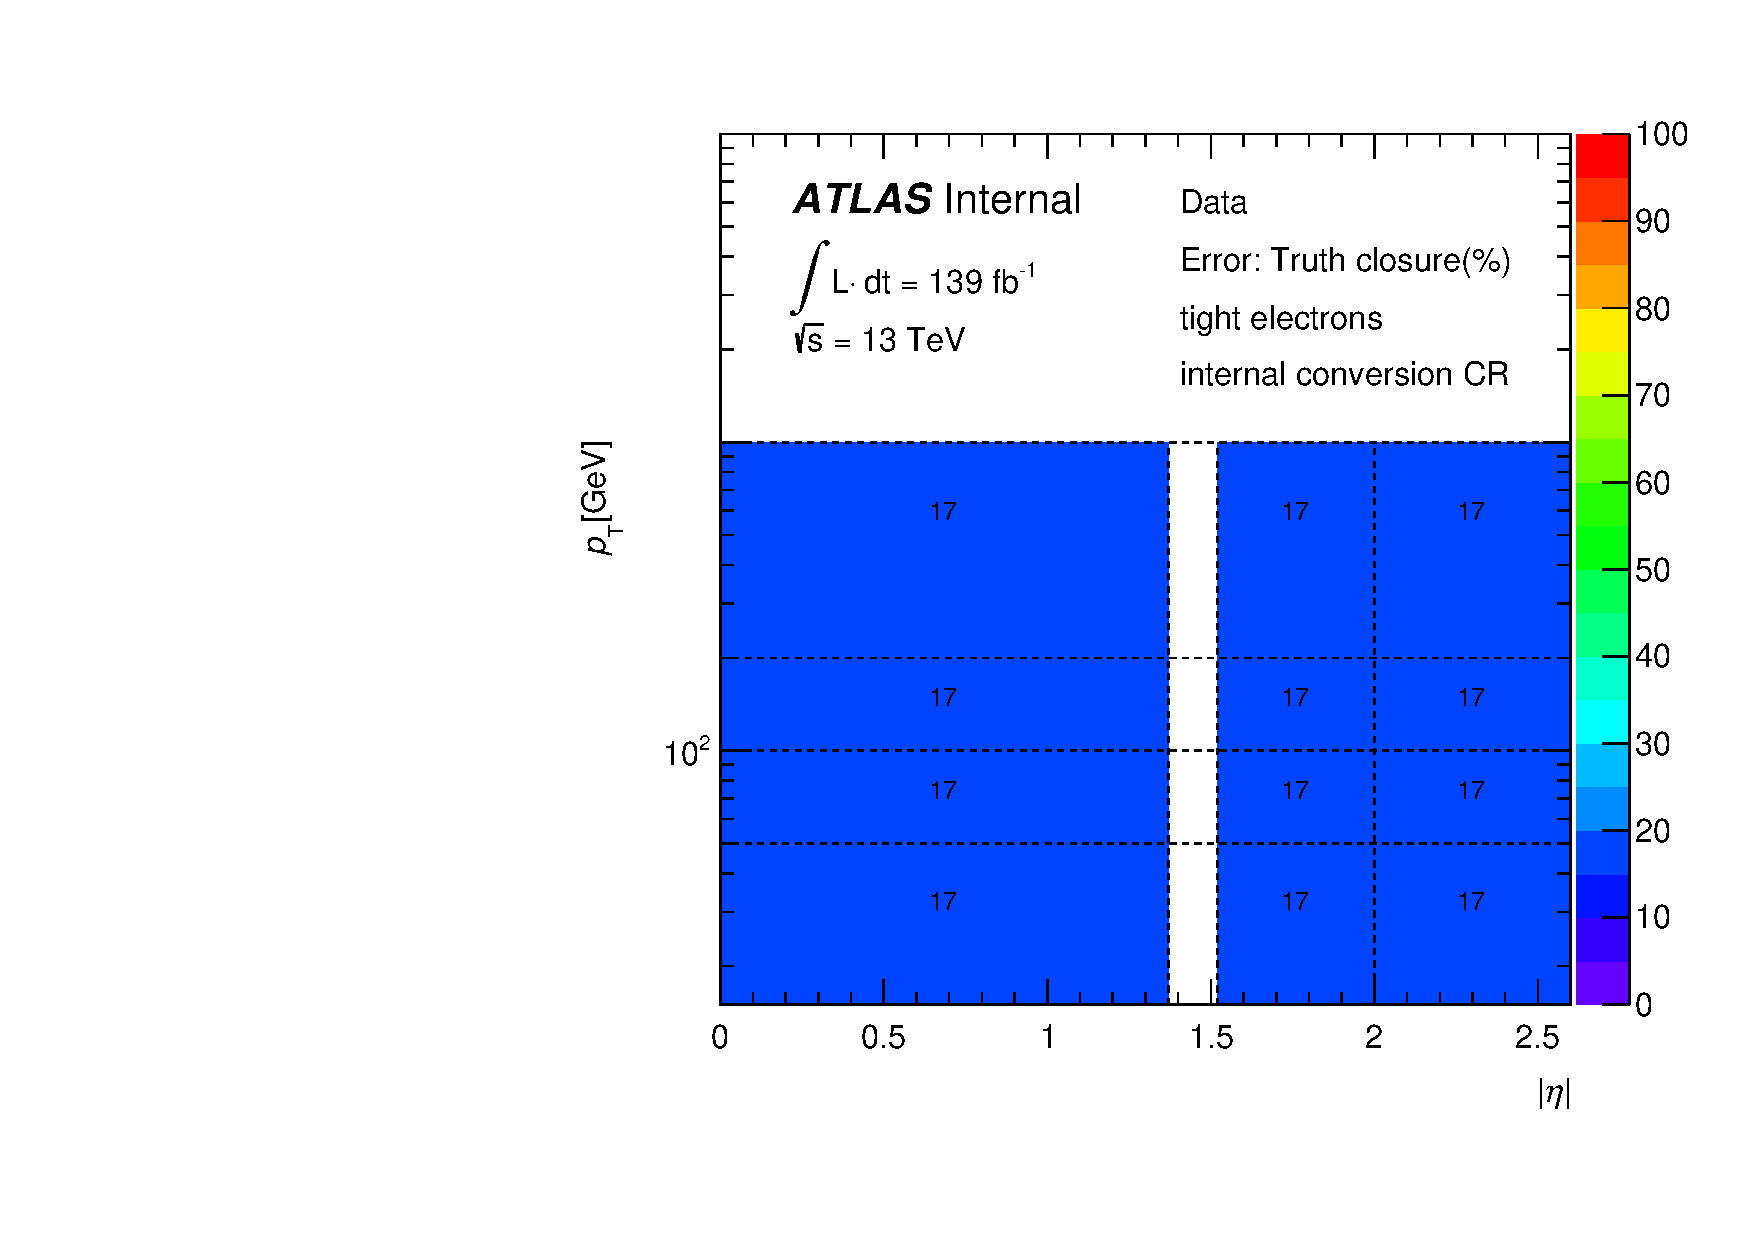
\includegraphics[width=0.45\textwidth]{figures/qmisid/syst_Data_Truthclosure_tight_intcr}\\
  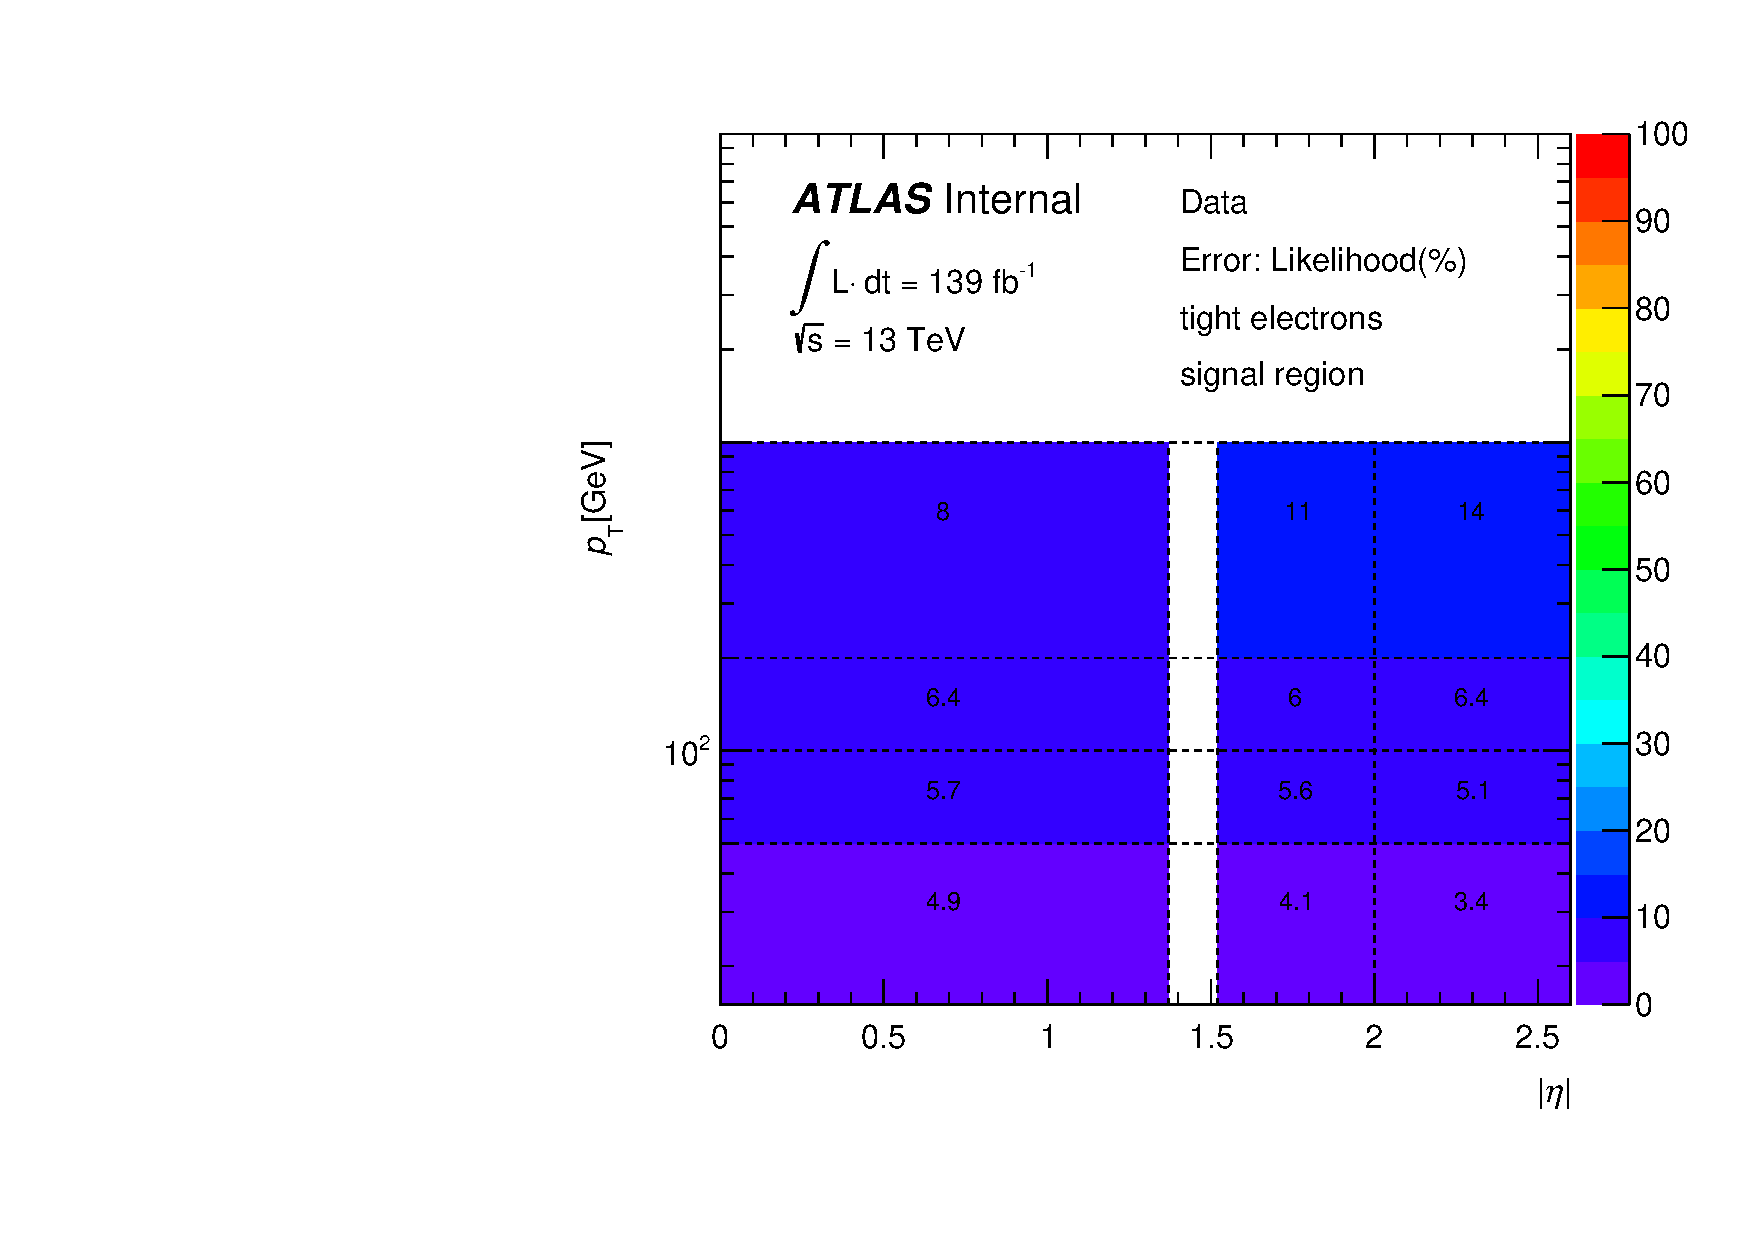
\includegraphics[width=0.45\textwidth]{figures/qmisid/syst_Data_Likelihood_tight_sr}
  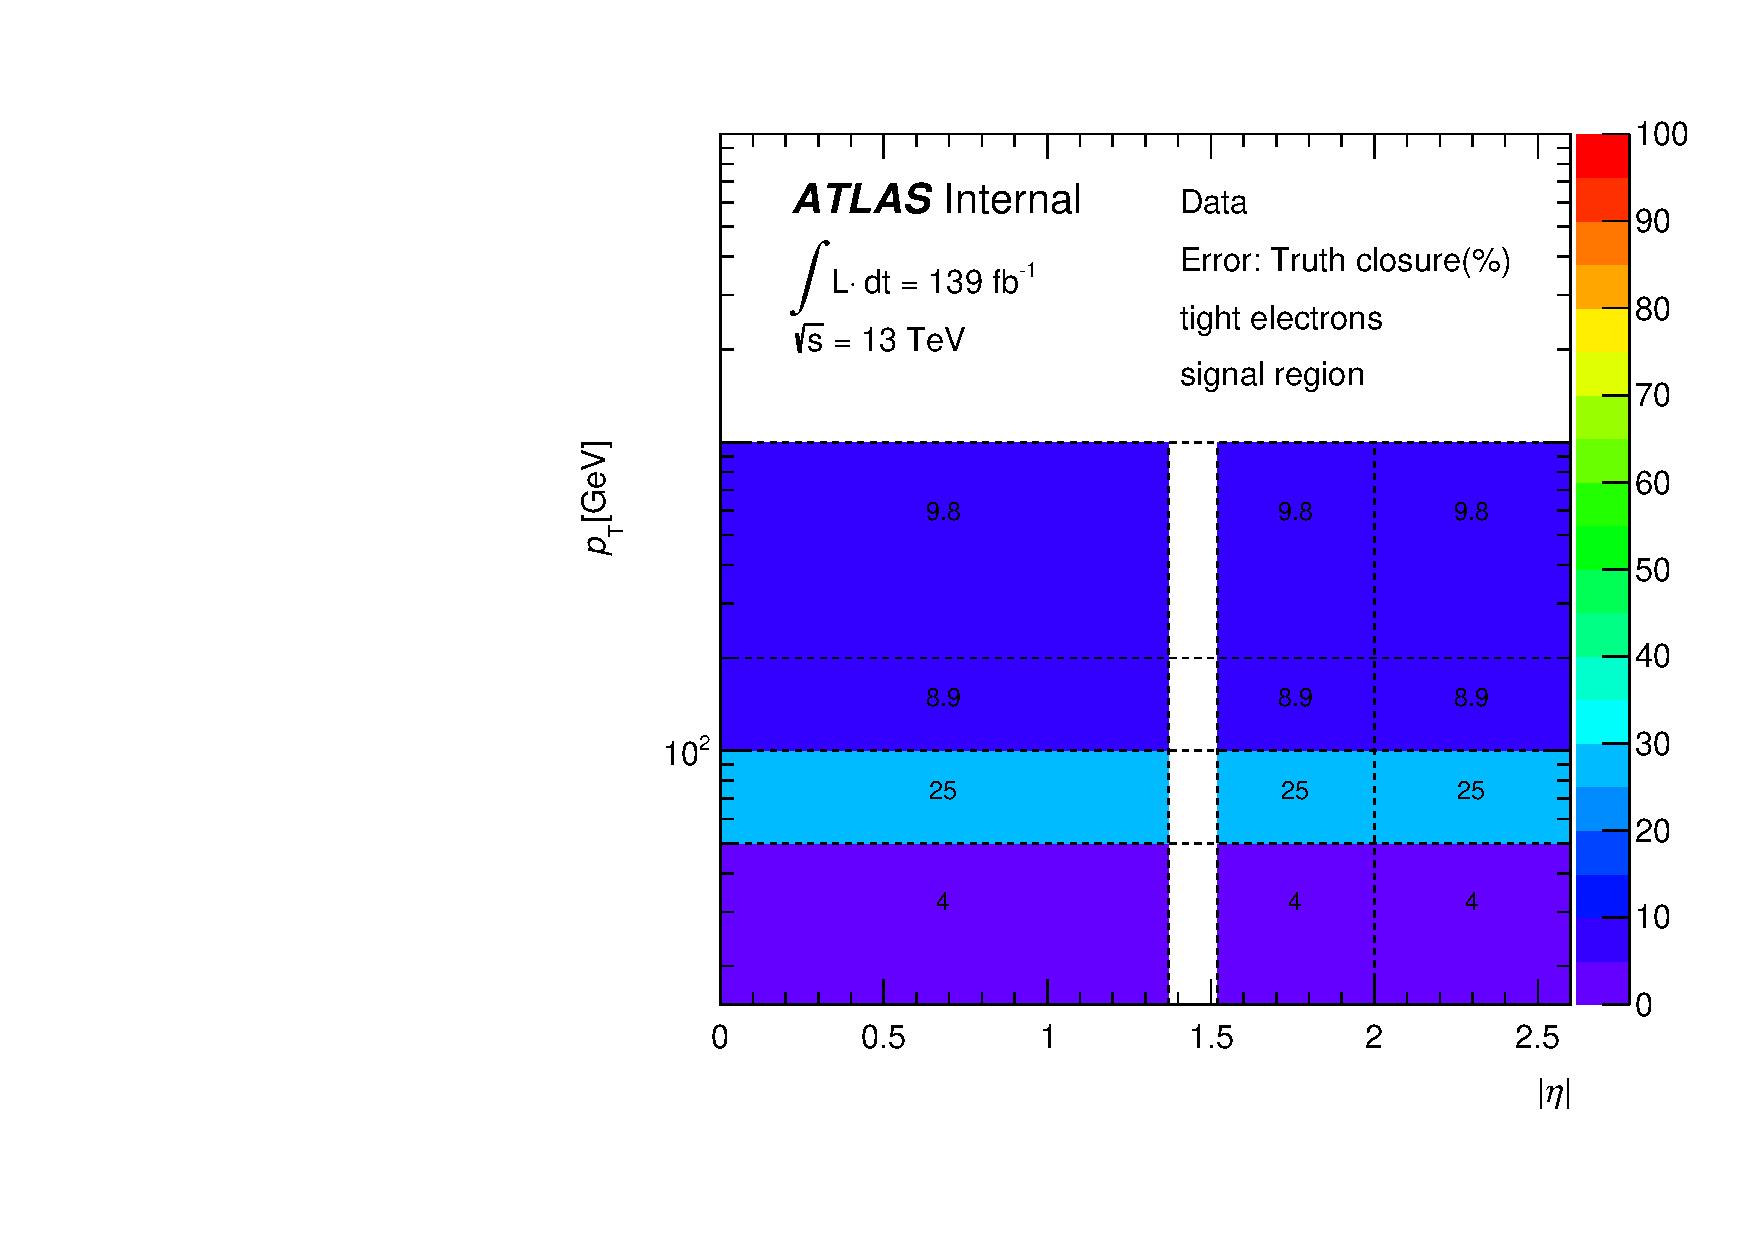
\includegraphics[width=0.45\textwidth]{figures/qmisid/syst_Data_Truthclosure_tight_sr}
  \caption{ \label{fig:QMisID:systa} Left: systematic uncertainty (\%), introduced from the statistical size of the control 
            region of the data that is used in the likelihood method, in bins of $|\eta|$ and $\pT$. Right: systematic uncertainty 
            (\%), introduced from the comparison of rates obtained from simulated $Z\rightarrow ee$ events with the likelihood 
            method to truth-based rates.}
  \end{center}
\end{figure}

\begin{figure}[p!]
  \begin{center}
  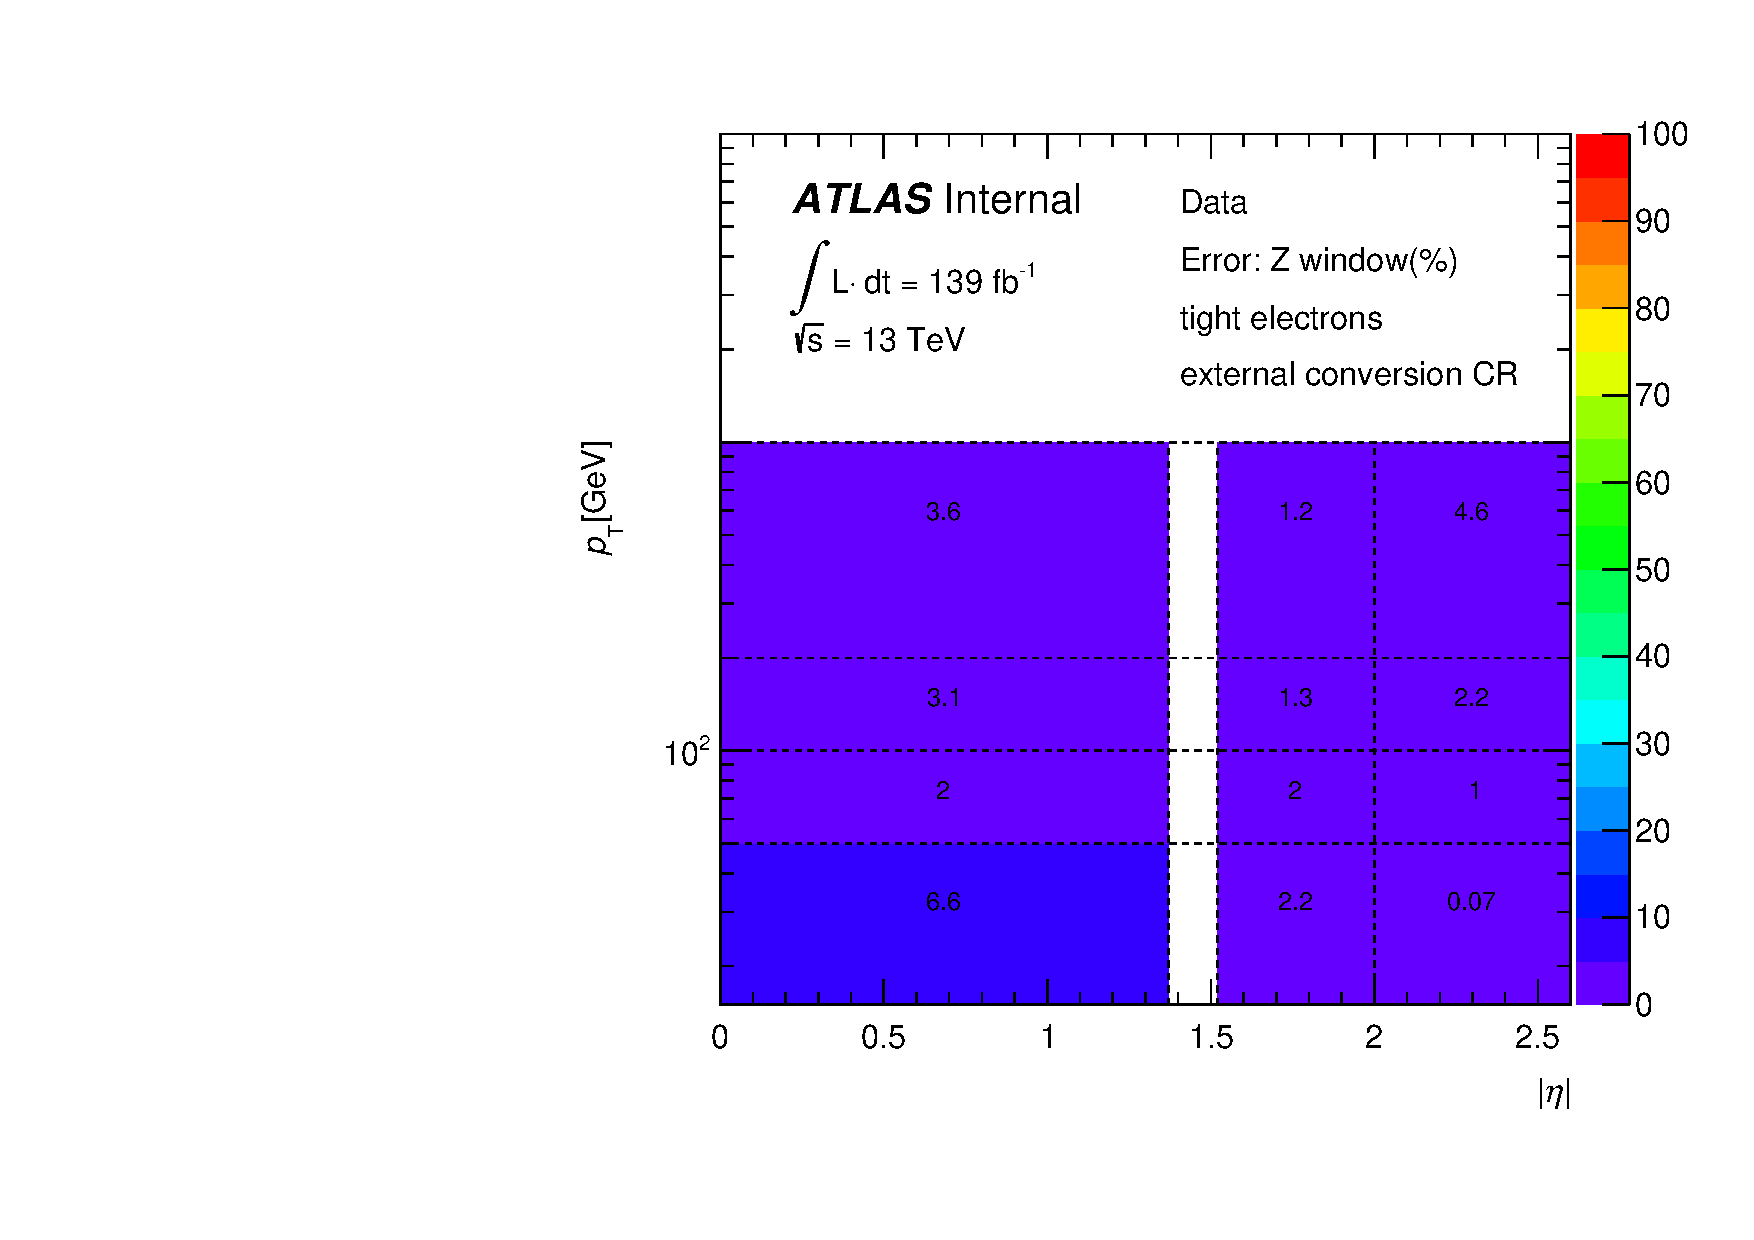
\includegraphics[width=0.45\textwidth]{figures/qmisid/syst_Data_Zwindow_tight_extcr}
  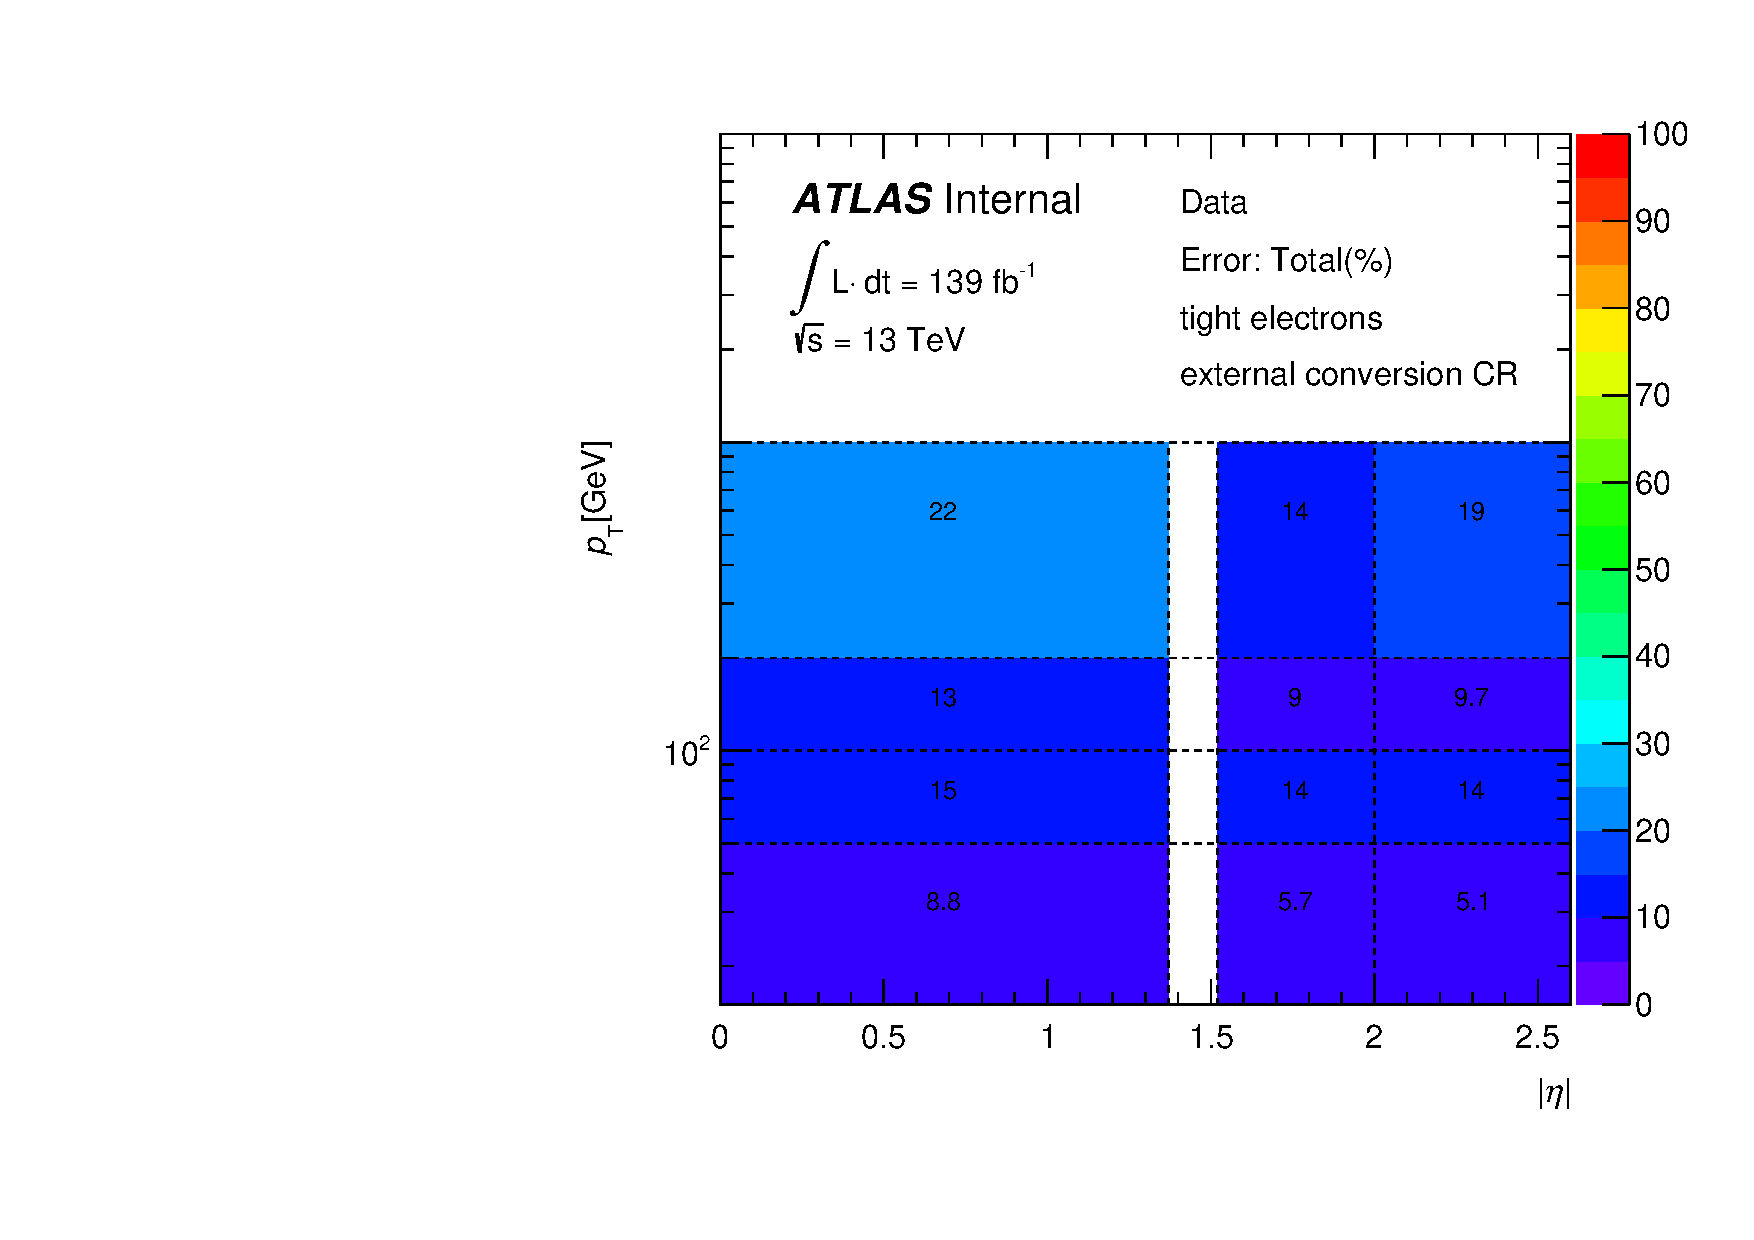
\includegraphics[width=0.45\textwidth]{figures/qmisid/syst_Data_Total_tight_extcr}\\
  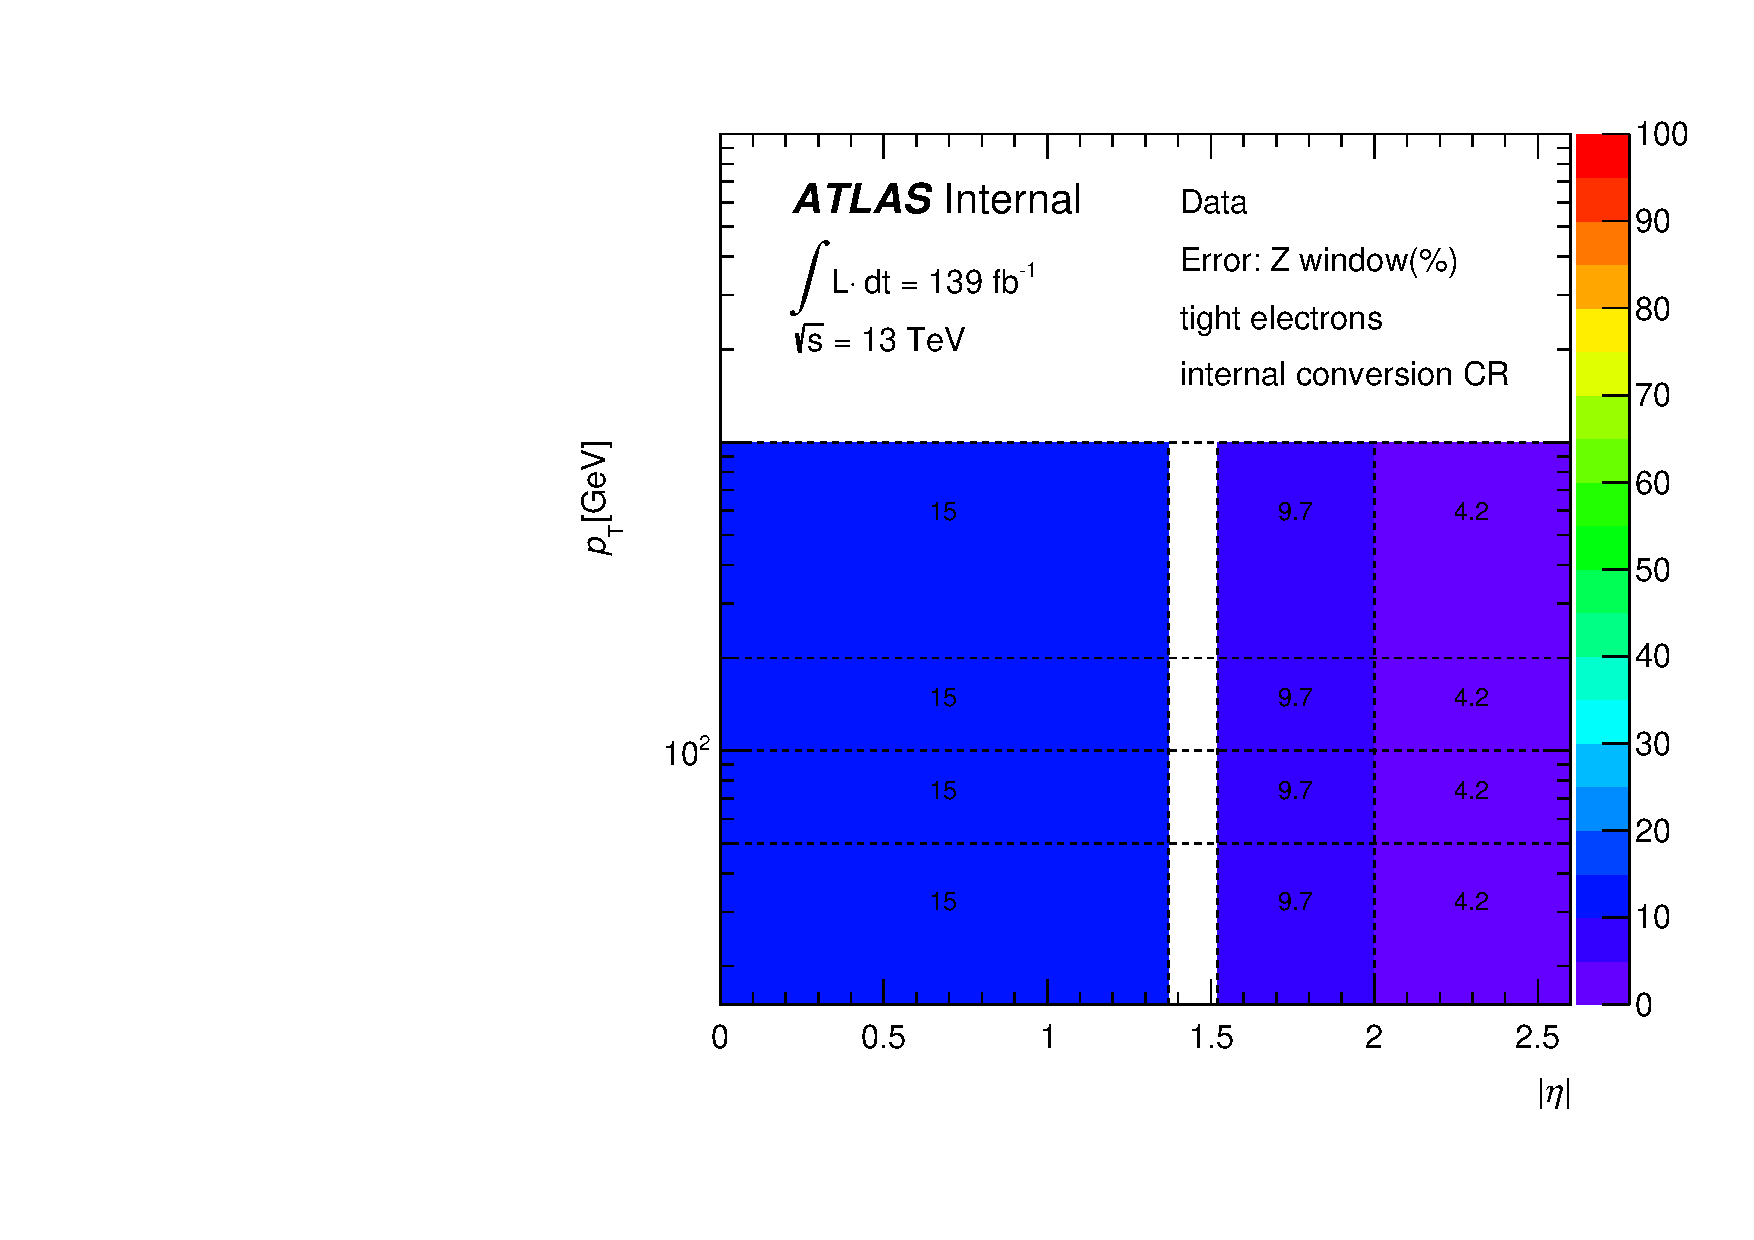
\includegraphics[width=0.45\textwidth]{figures/qmisid/syst_Data_Zwindow_tight_intcr}
  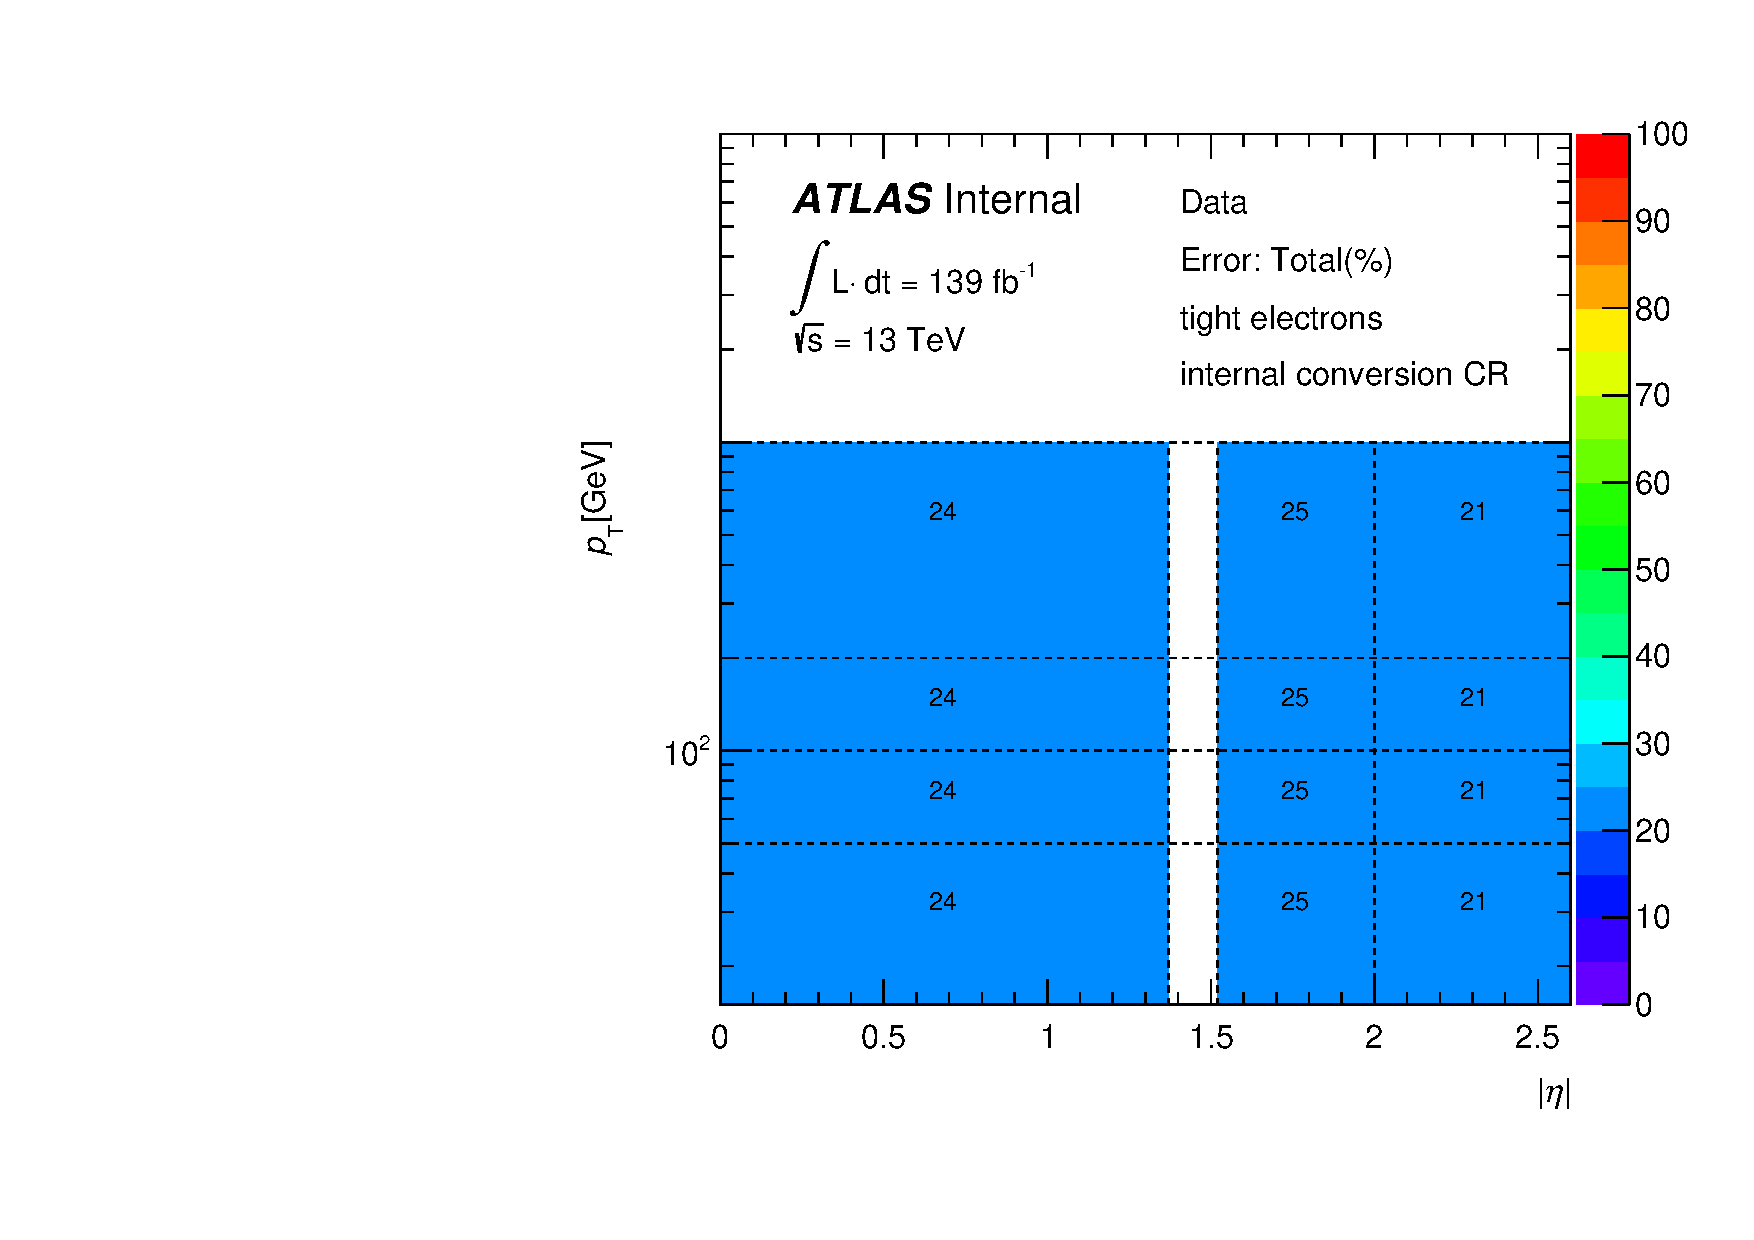
\includegraphics[width=0.45\textwidth]{figures/qmisid/syst_Data_Total_tight_intcr}\\
  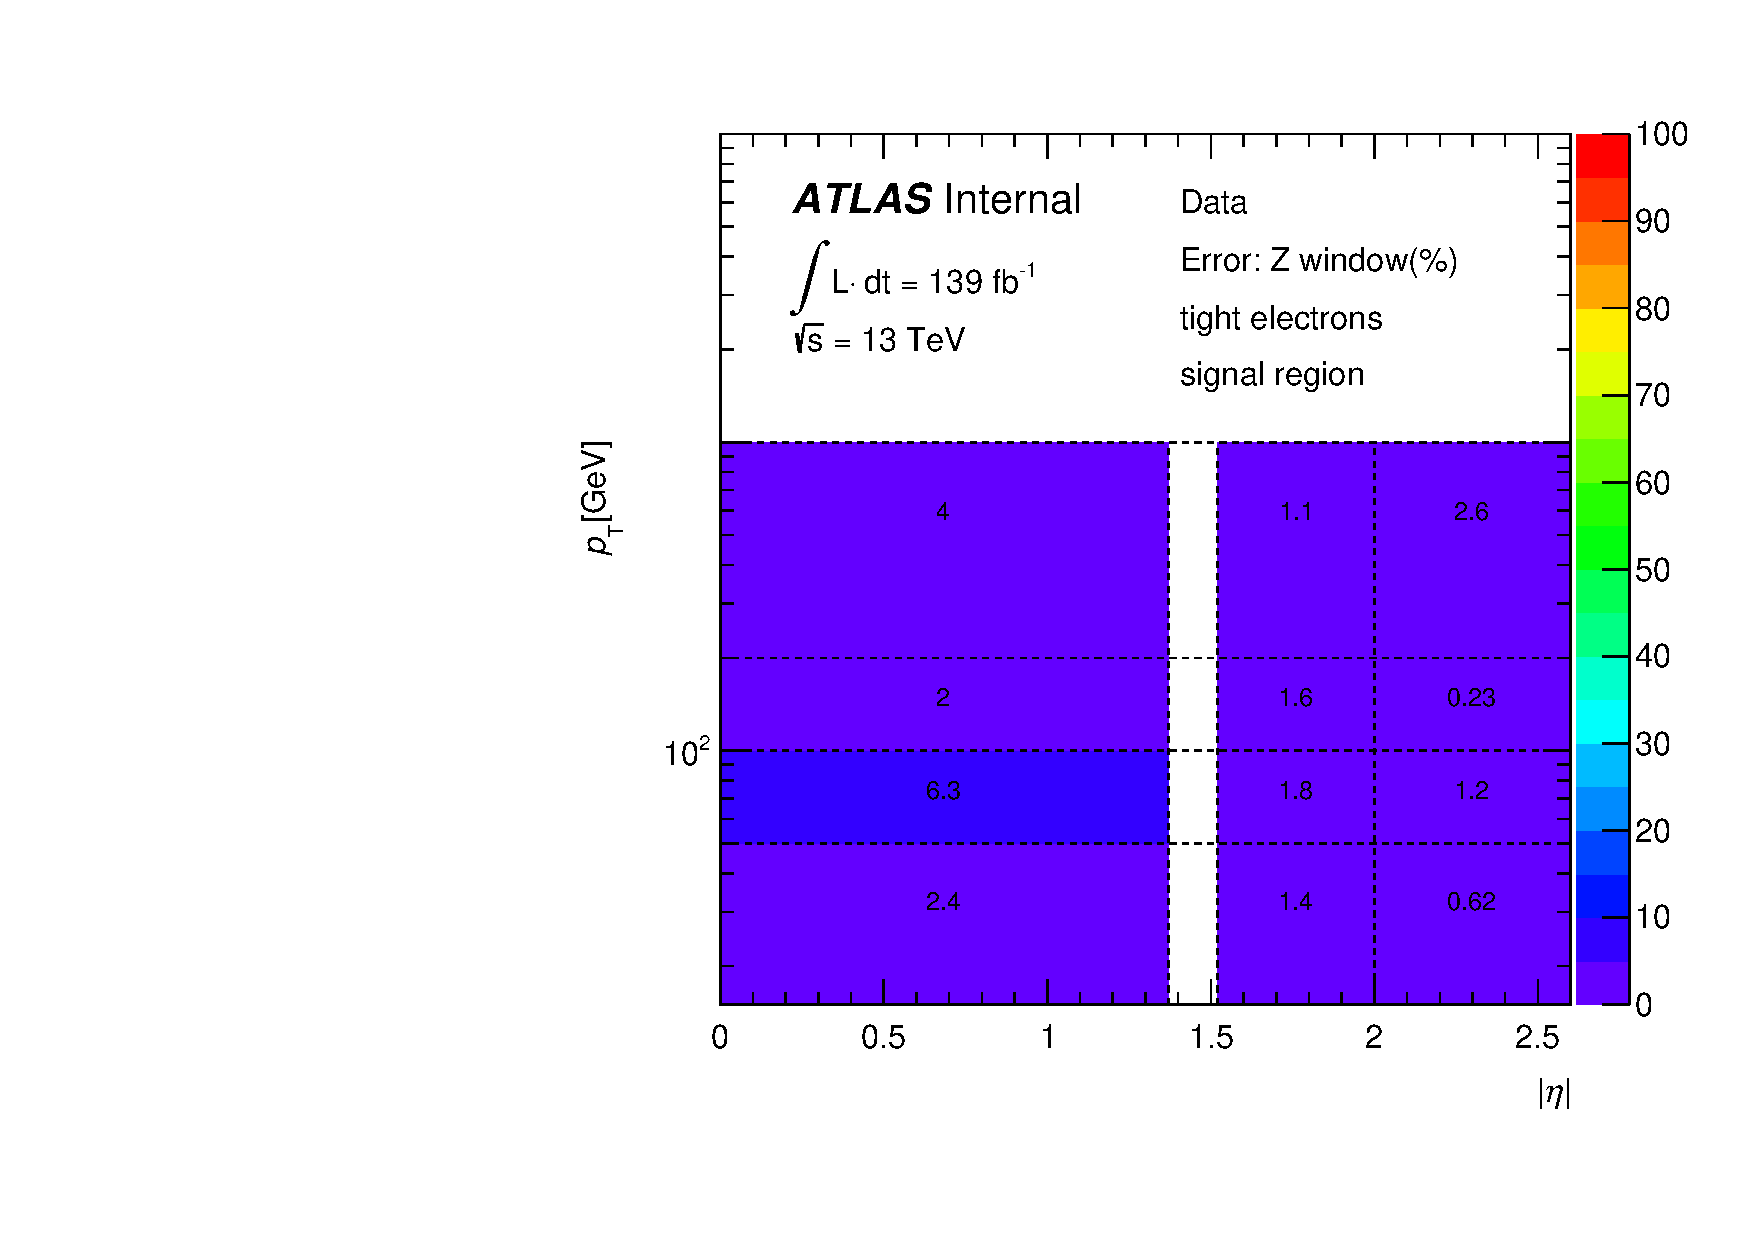
\includegraphics[width=0.45\textwidth]{figures/qmisid/syst_Data_Zwindow_tight_sr}
  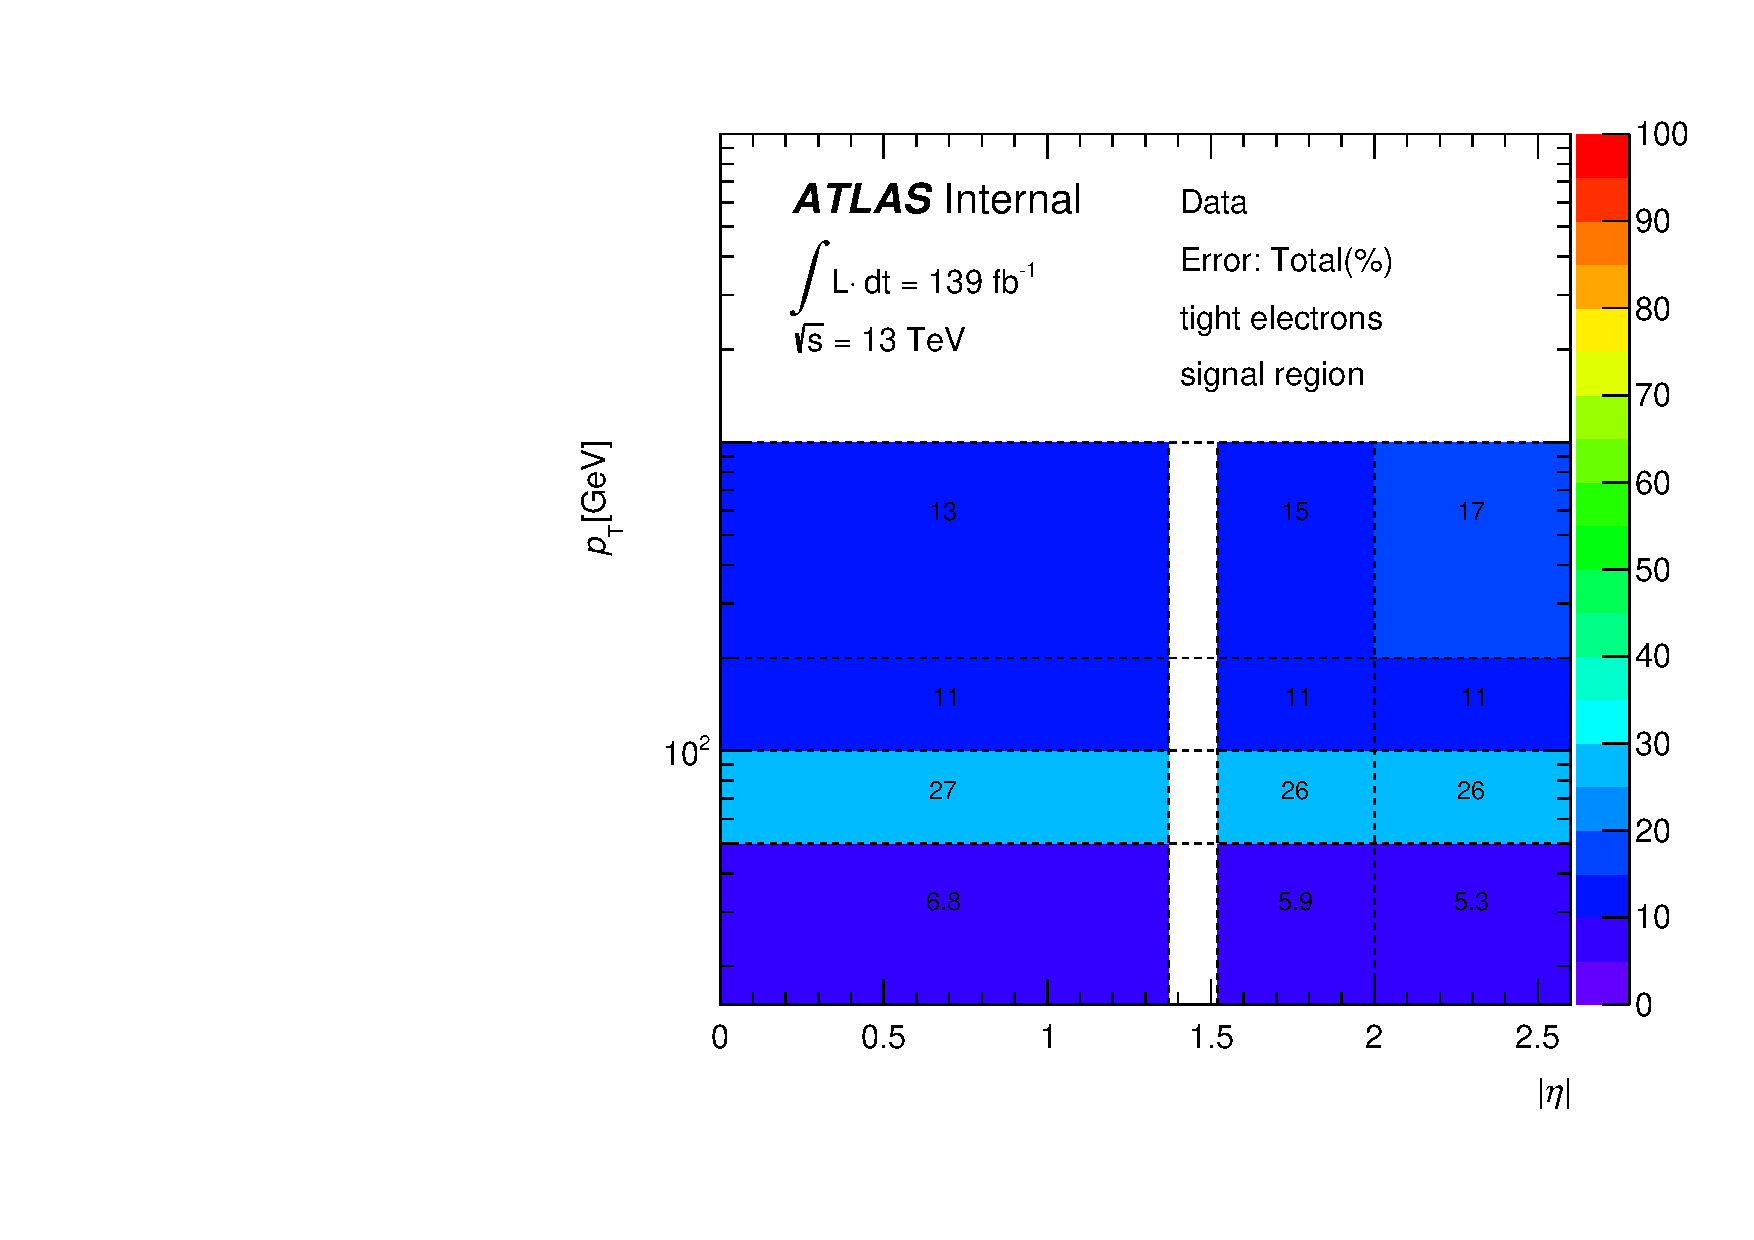
\includegraphics[width=0.45\textwidth]{figures/qmisid/syst_Data_Total_tight_sr}
  \caption{ \label{fig:QMisID:systb} Left: systematic uncertainty (\%), introduced from the variation of the $m_{Z}$ window
  (and its sidebands) that is used to obtain the rates, in bins of $|\eta|$ and $\pT$. Right: Total systematic uncertainty (\%).}
  \end{center}
\end{figure}

%~~~~~~~~~~~~~~~~~~~~~~~~~~~~~~~~~~~
\subsubsection{Closure test}
\label{Sec:closure}
%~~~~~~~~~~~~~~~~~~~~~~~~~~~~~~~~~~~

The rates are validated by comparing the estimated number of same-sign $ee$ events (using the QMisID rates on
opposite-sign events) to the measured number of same-sign events. In order to increase the statistical
precision, this test is performed without any requirement regarding the number of jets. 
Figure\,\ref{fig:clData}, shows the expected distribution of $m_{ee}$ in the data, compared to the observation
(the latter also contains contributions from non-prompt electrons). 
After subtracting the non-prompt electron background using the sidebands, the
measured number of same-sign events in the $m_{Z}$ window is found to be 6474
(1076) for events with at least 1 jet (3 jets) while the expectation is
$6951 \pm 1024$ ($1156 \pm 95$). The $\pT$ distribution (within the $m_{Z}$ window) is also presented 
in figure\,\ref{fig:clData}, showing agreement between the measurement and the prediction, which however begins 
to deteriorate in the very high $\pT$ region, due to the fact that the region above 200\,GeV is described by an 
inclusive QmisID rate.

The respective comparison with $Z$+jets MC (in which the non-prompt contribution is removed using the truth 
information) is shown in figure\,\ref{fig:clMC}.

\begin{figure}[htb!]
\centering
  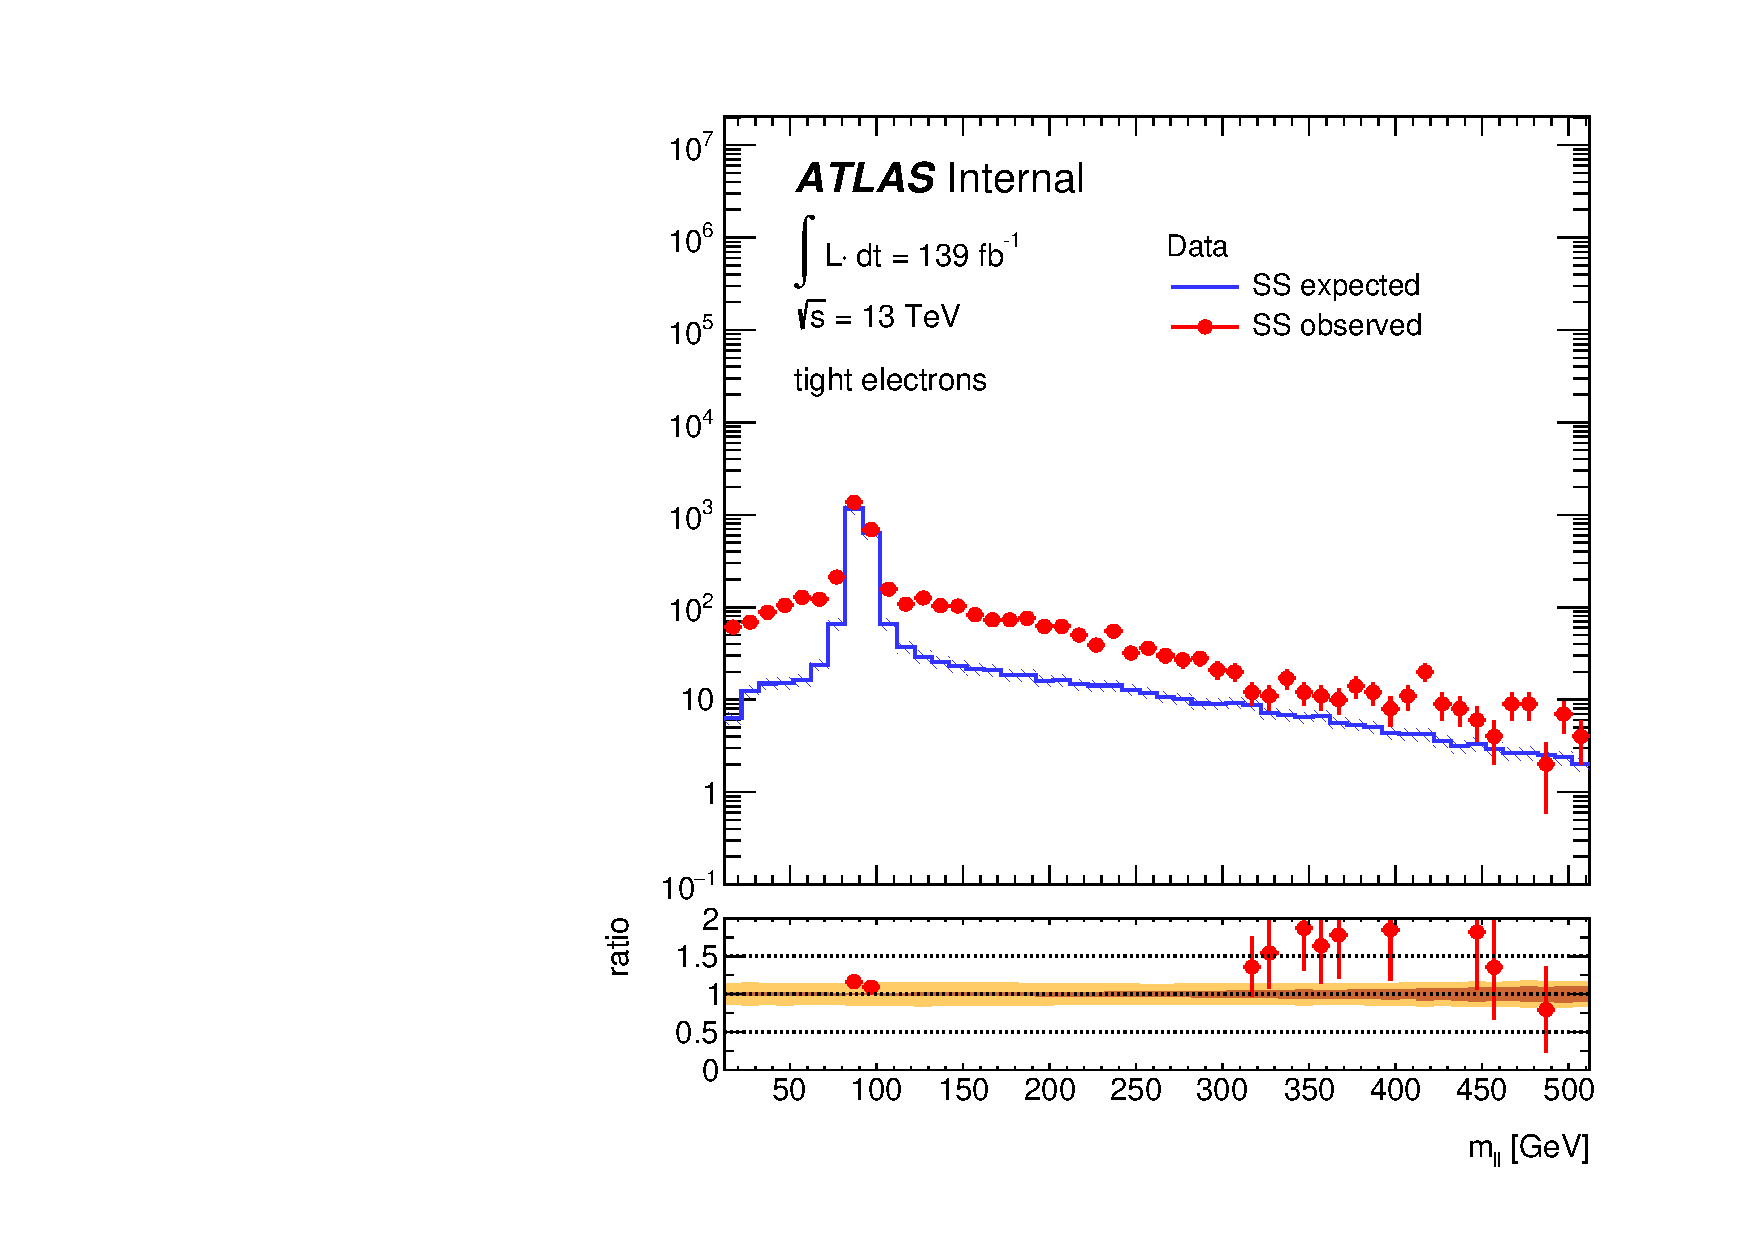
\includegraphics[width=0.45\textwidth]{figures/qmisid/valid_MlltightData}
  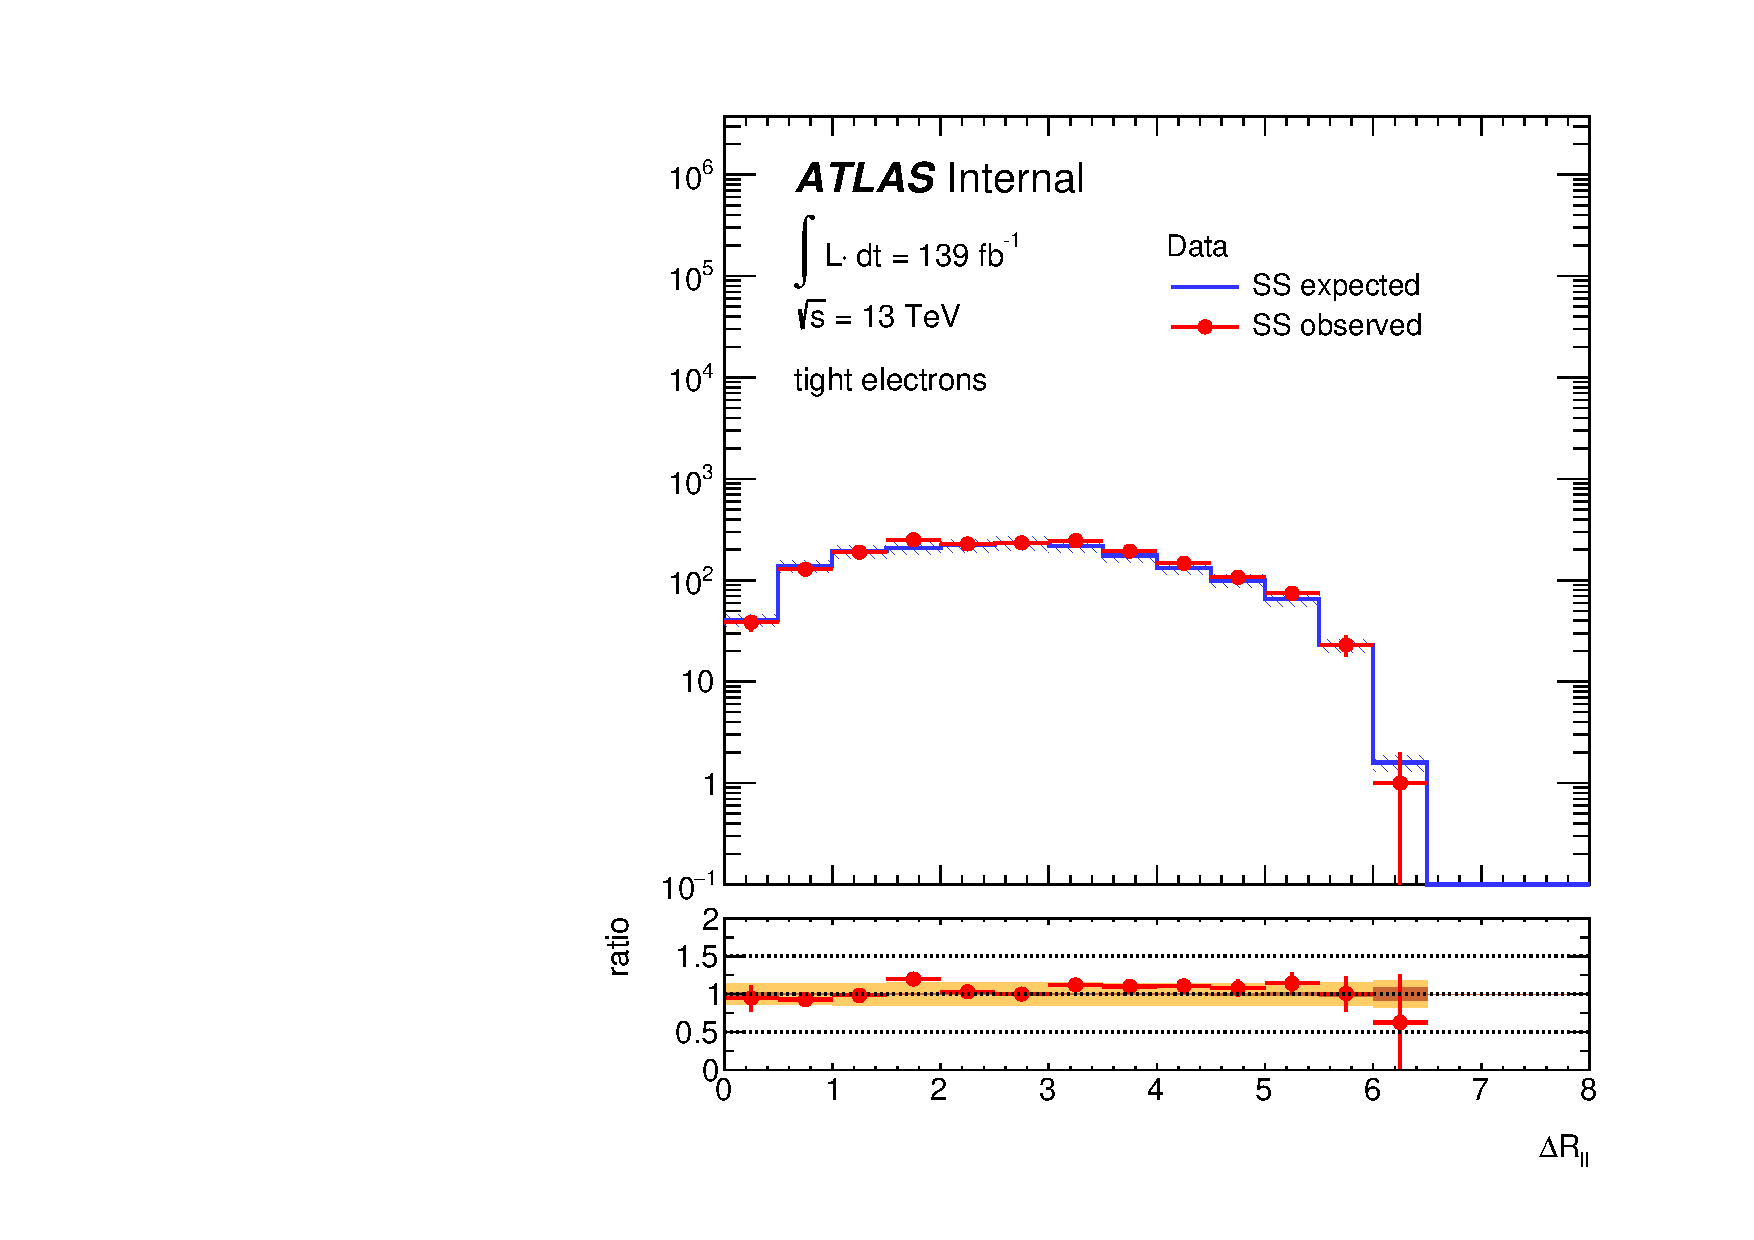
\includegraphics[width=0.45\textwidth]{figures/qmisid/valid_DRlltightData}\\
  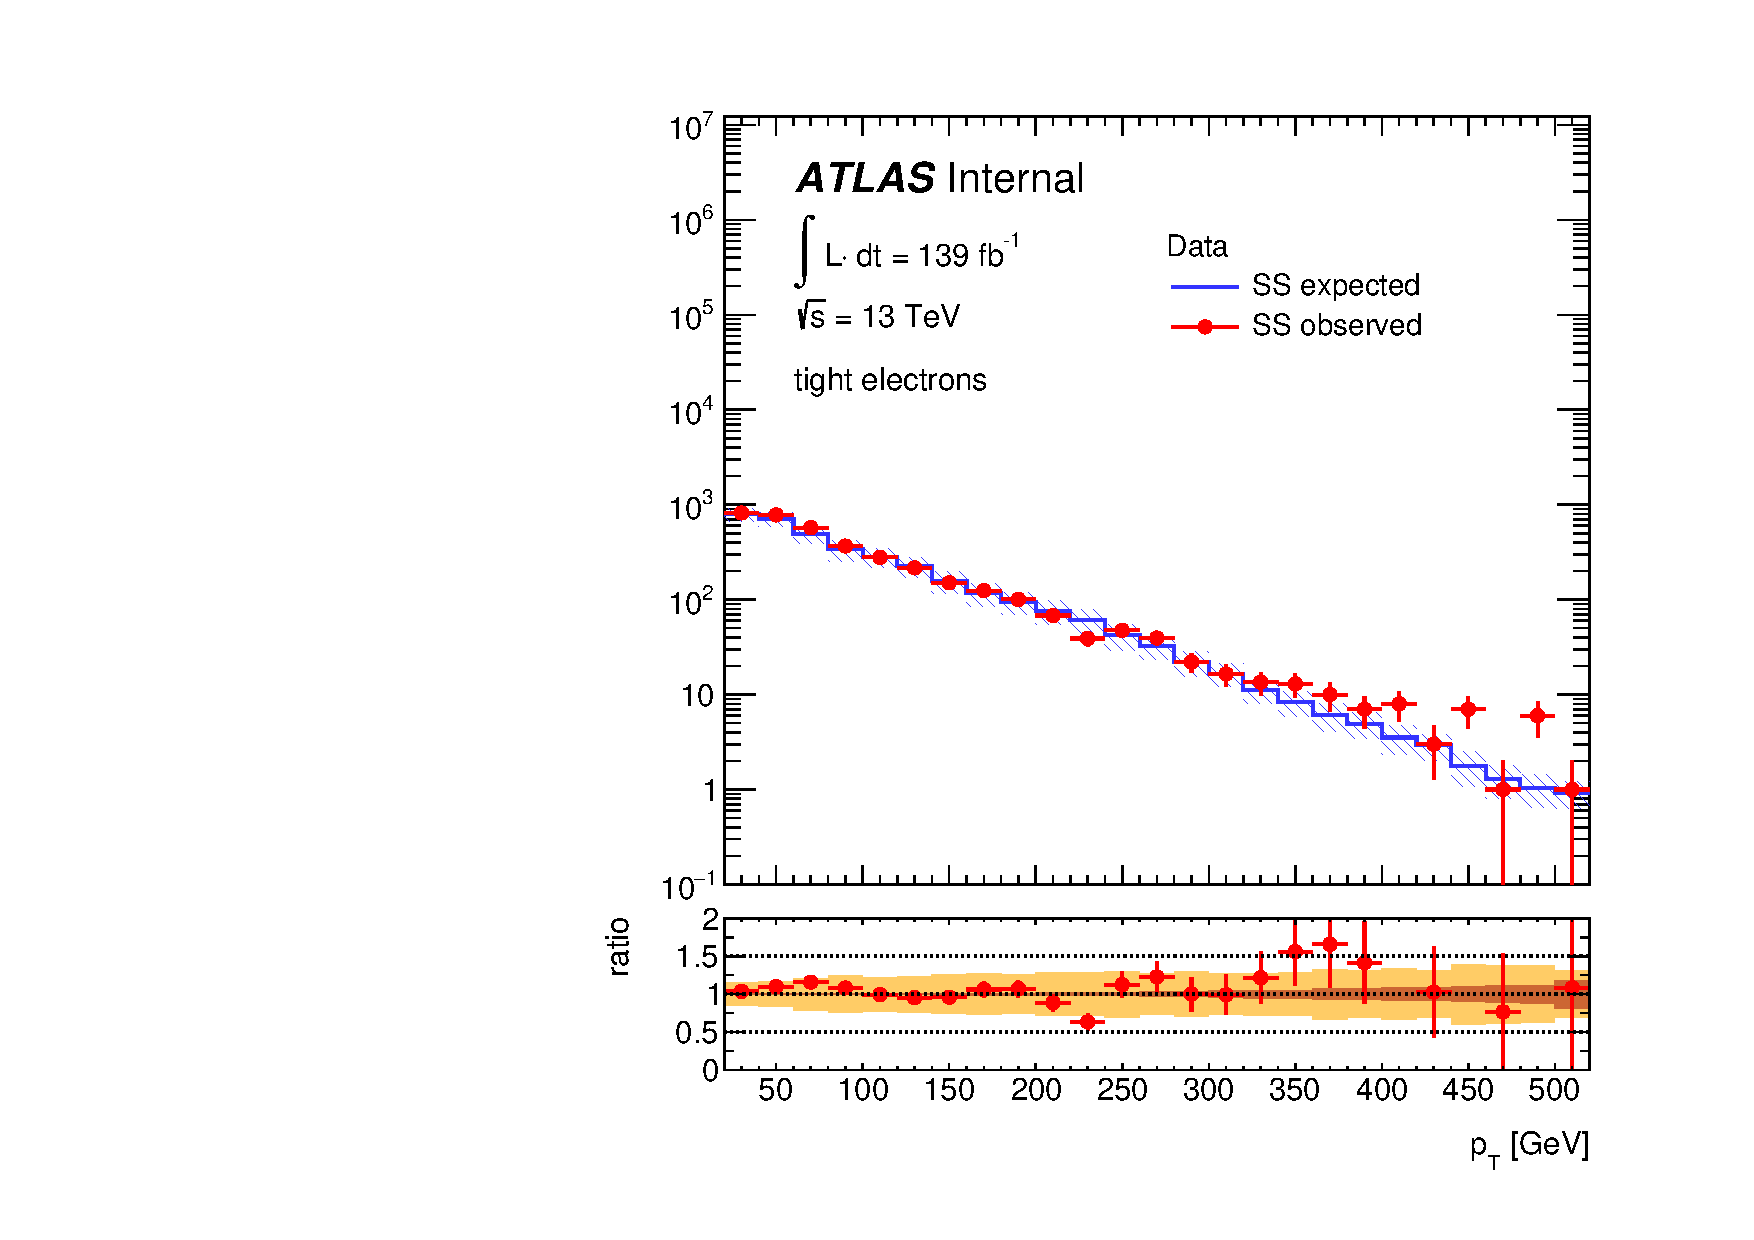
\includegraphics[width=0.45\textwidth]{figures/qmisid/valid_PttightData}
  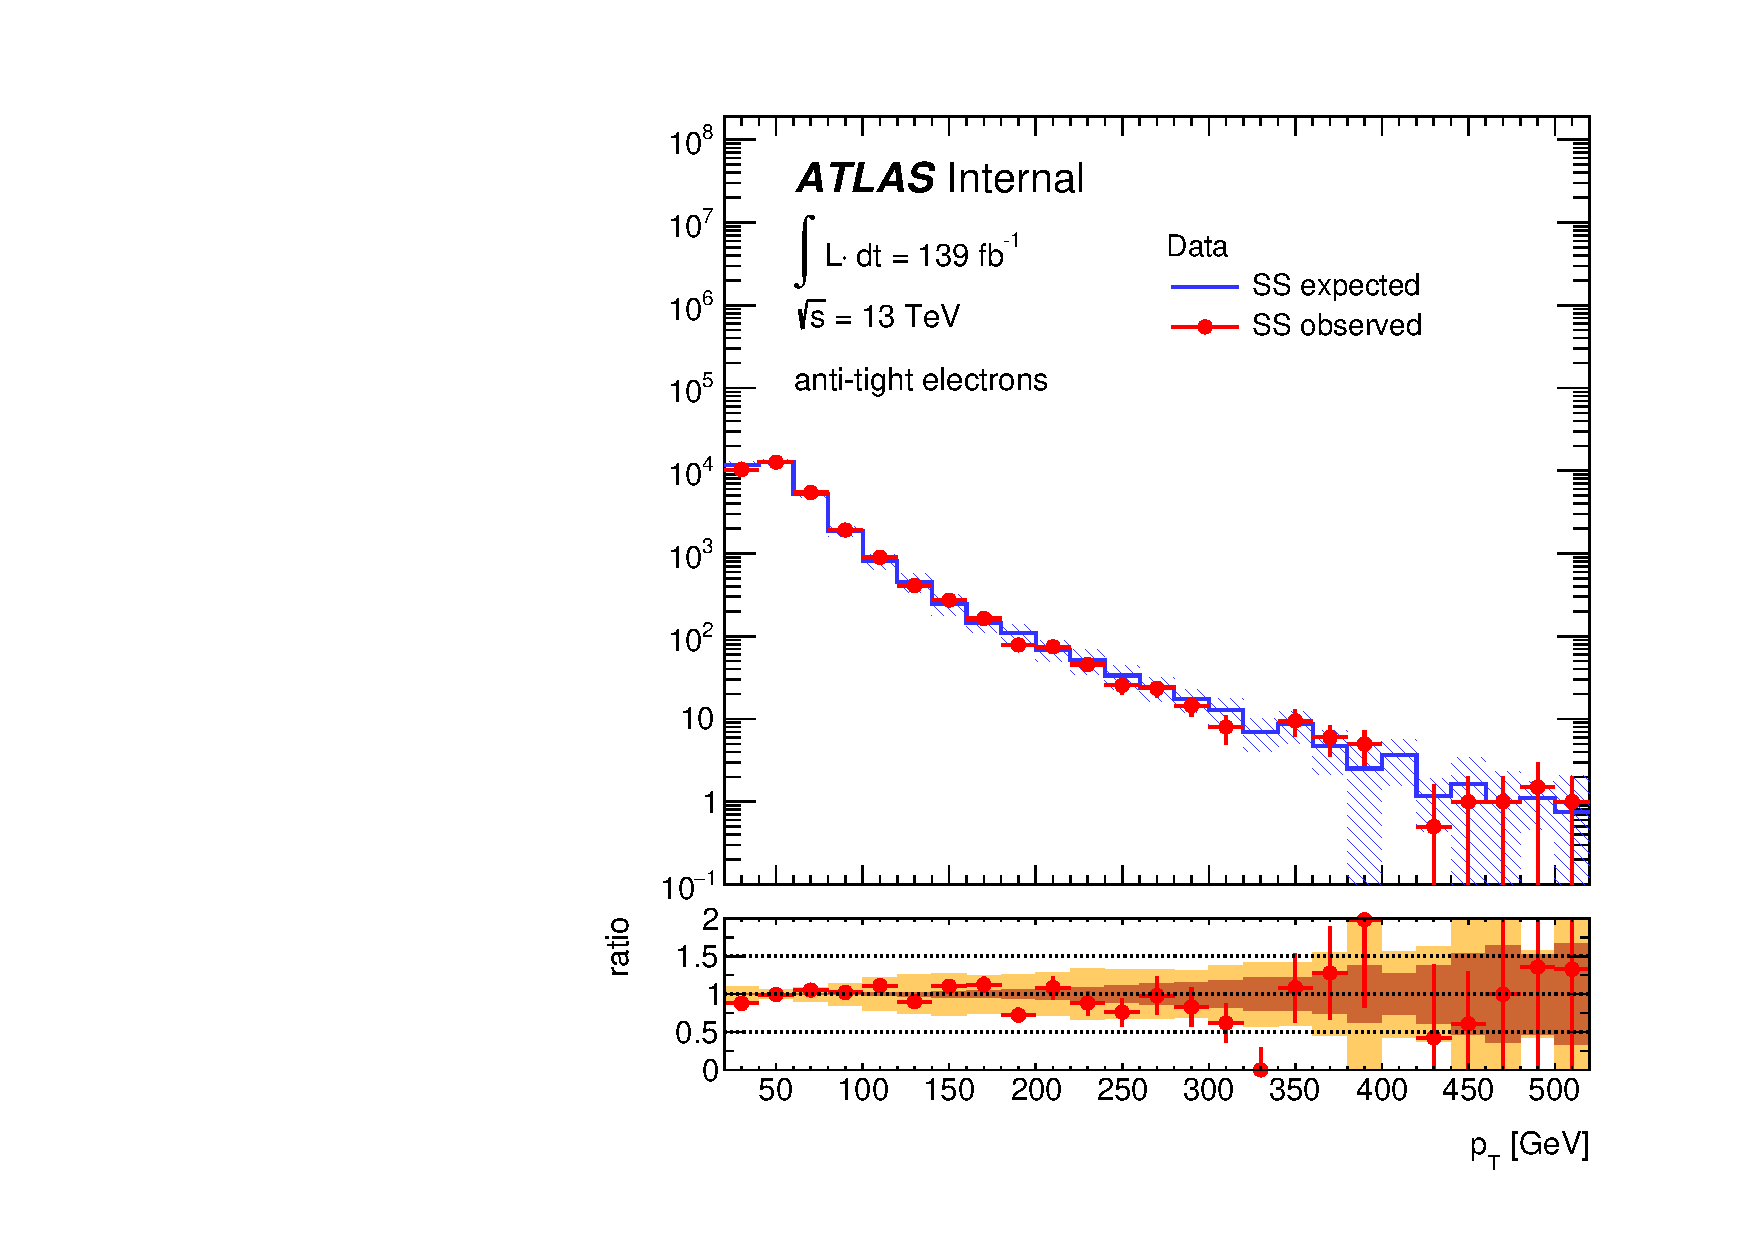
\includegraphics[width=0.45\textwidth]{figures/qmisid/valid_PtatightData}\\
  \caption{Comparison between the expected and observed $m_{ee}$, ${\Delta}R_{ee}$, $pT$ (tight) and $\pT$ (anti-tight) of same-sign electrons.  The dashed bands represent the total (statistical + systematic) uncertainty of the estimation. The comparison is shown for data events. The observed $m_{ee}$ distribution includes the contribution of fake electrons, which are later subtracted by using the sidebands.\label{fig:clData}}
\end{figure}


\begin{figure}[htb!]
\centering
  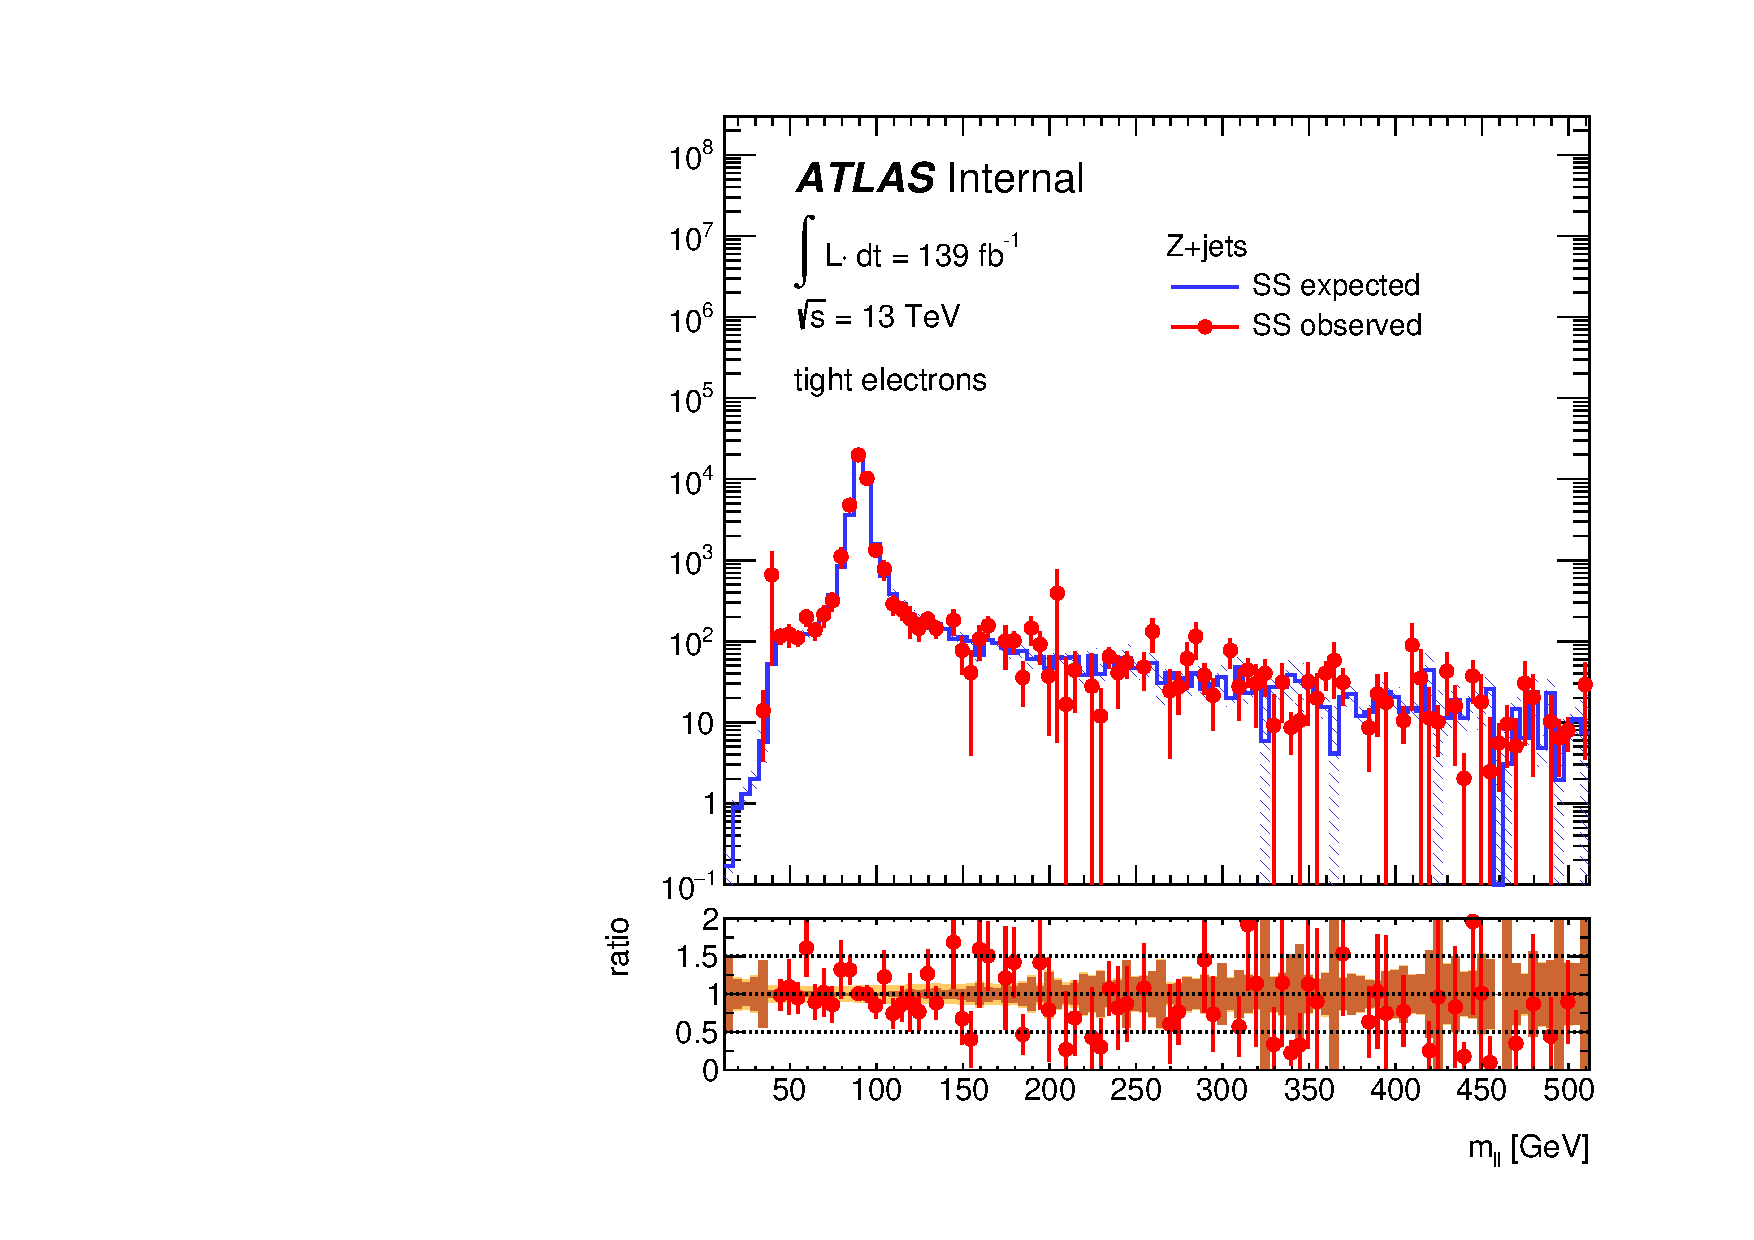
\includegraphics[width=0.45\textwidth]{figures/qmisid/valid_MlltightZ}
  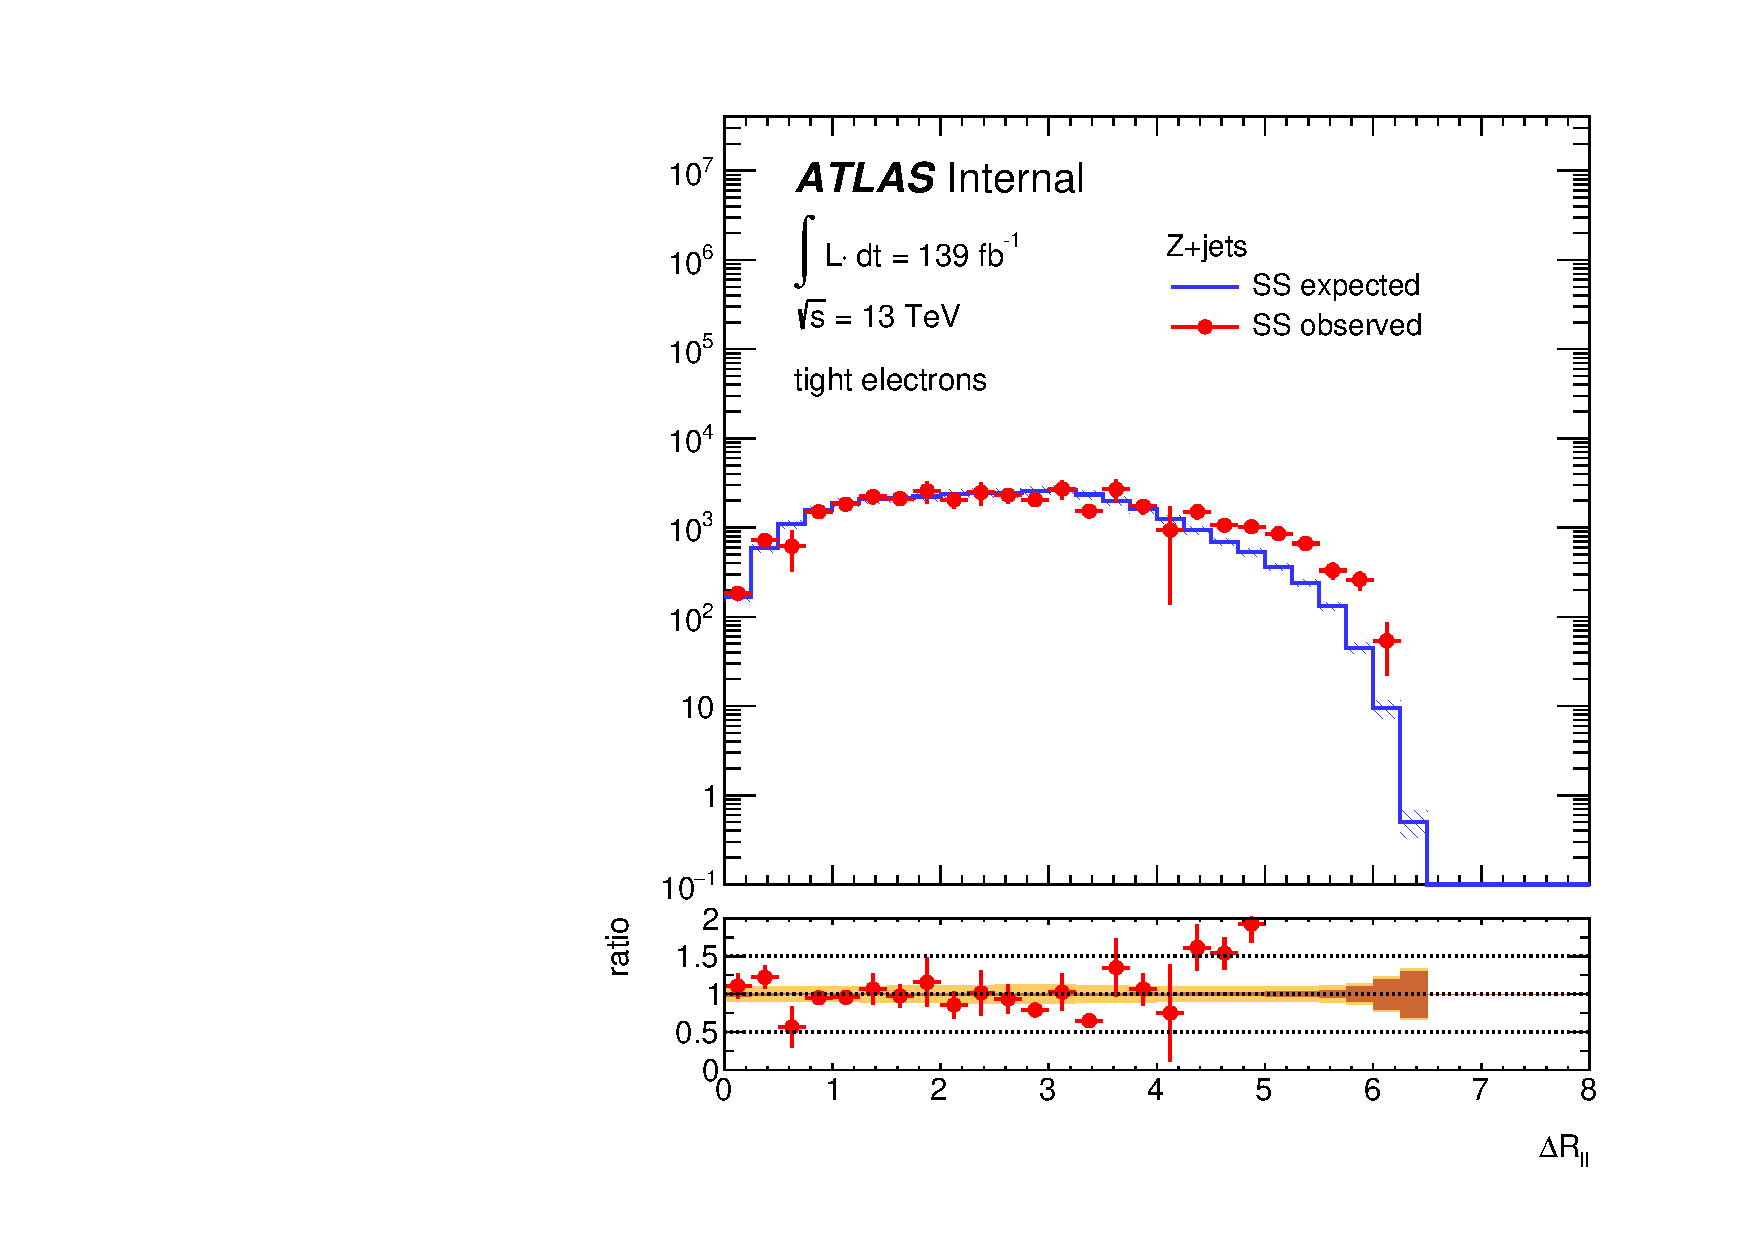
\includegraphics[width=0.45\textwidth]{figures/qmisid/valid_DRlltightZ}\\
  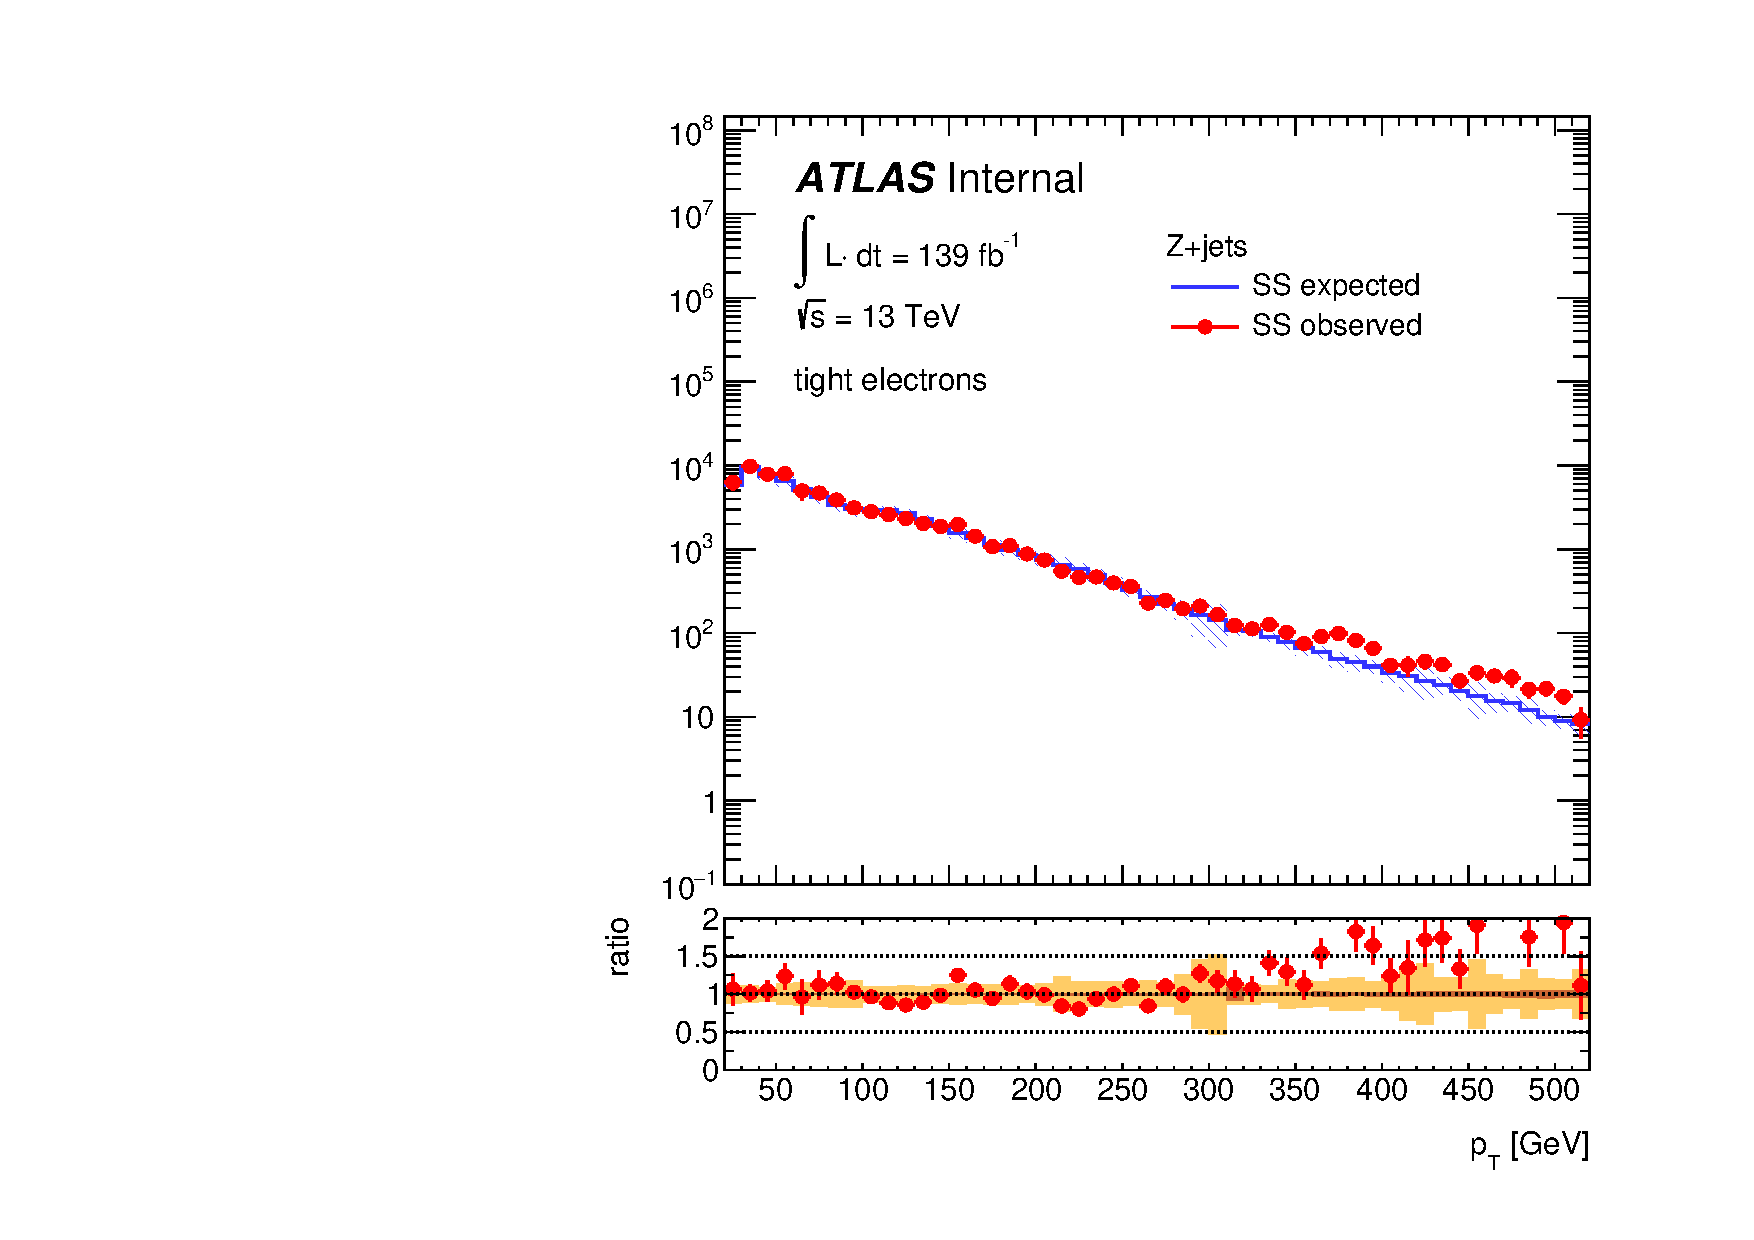
\includegraphics[width=0.45\textwidth]{figures/qmisid/valid_PttightZ}
  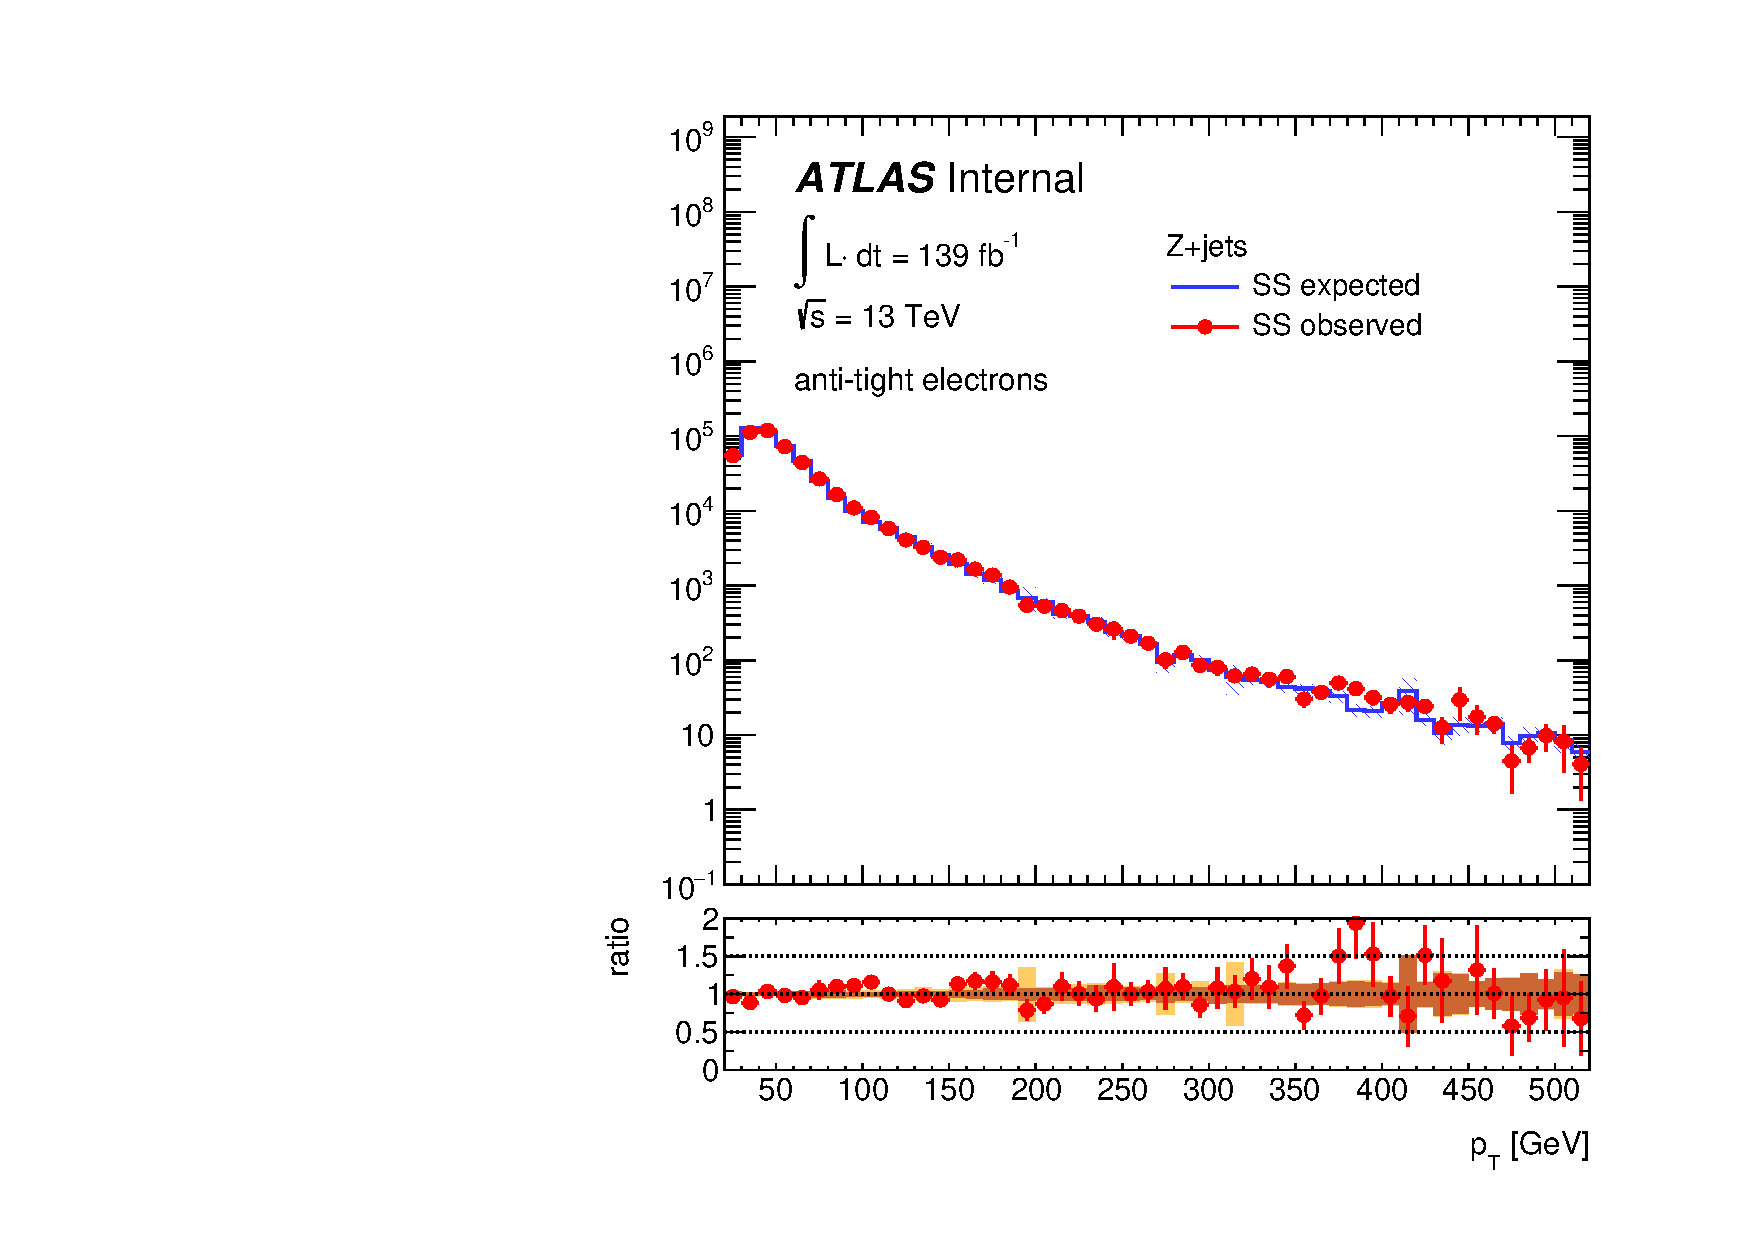
\includegraphics[width=0.45\textwidth]{figures/qmisid/valid_PtatightZ}\\
  \caption{Comparison between the expected and observed $m_{ee}$,
${\Delta}R_{ee}$, $\pT$ (tight) and $\pT$ (anti-tight) of same-sign electrons.
The dashed bands represent the total (statistical + systematic) uncertainty of the estimation.
 The comparison is shown for $Z$+jets events. Fake electrons are removed from
 the sample by using the truth information.\label{fig:clMC}} 
\end{figure}


\clearpage
\section{The Analysis of 3 Lepton Channel }
\label{sec:AnaThreeL}
Add the text for 3L



\clearpage
\section{The Analysis of 4 Lepton Channel }
\label{sec:AnaFourL}
Add the text for 4L



\clearpage
\section{The Analysis of $\gamma\gamma$+Lepton Channel }
\label{sec:AnaYYL}
Add the text for 3L



\clearpage
\section{The Analysis of $\tau$ Channels }
\label{sec:taus}
Add the text for $\tau$ channels



\clearpage
\section{The Analysis of $bb$ + 4l Channels }
\label{sec:bb4l}

\subsection{Analysis strategy}
\label{subsec:ana}

This analysis relies on the use of a multivariate discriminant designed to select candidate events consistent with non-resonant $HH$ production. To construct such a discriminant, a signal region is defined with some event selection criteria. Section \ref{subsubsec:pre-selection} describes these signal region selection criteria. Section \ref{subsubsec:mva} describes the architecture and the training of the Boosted Decision Tree (BDT) classifier from which the discriminant is constructed. Section \ref{subsubsec:bkg} describes the final background estimation procedure.

\subsubsection{Event selection}
\label{subsubsec:pre-selection}

To define the signal criteria, the analysis has some further requirements on each event. These events are triggered by any of the standard single electron and single muon, or di-leptons. Then trigger matching is applied to data and MC, requiring any of the selected leptons to be close to the corresponding trigger lepton within $\Delta{R}<0.1$.

In $4l+b\bar{b}$ channel, signal event are selected with exactly four leptons. The four leptons are sorted by $p_{T}$ number. Either of the third lepton and the forth lepton, with the third and forth highest $p_{T}$, is required to pass the $PflowLoose$ isolation working point. This loose selection can give a acceptable background rejection and good signal efficiency.

A angular separation of $\Delta{R}(l_{i},l_{j})=\sqrt{(\eta_{i}-\eta_{j})^{2}+(\phi_{i}-\phi_{j})^{2}}<0.1$ is required between any of lepton pairs.

In each quadruplet, the $p_{T}$ thresholds for the three leading leptons are 20,15 and 10 GeV.

The invariant mass of the $OSSF$ lepton pairs in each quadruplet is calculated. The lepton pair with invariant mass closest to the nominal $Z$ boson mass is selected as the leading lepton pair. The two remaining leptons are also required to be $OSSF$ and form the sub-leading lepton pair.

All the $OSSF$ lepton pairs are required to have invariant mass large than 5 GeV to veto the $J/\Psi$ decay.

Events are selected with at least two jets. The $DL1r$ algorithm is used to identify jets containing $b$-hadrons ($b$ jets). Events containing at least one $b$ jets are selected by requiring the number of jets passing a $DL1r$ working point, which gives a $b$-tagging efficiency of 77\%, no less than one.

Finally the invariant mass of the four leptons must satisfy 107 GeV$<M_{\rm 4l}<$ 133 GeV to select a on-shell Higgs decay. A comprehensive summary of all the cuts and requirements used in the event selection is shown in Table \ref{Tab.pre-selection}.

\begin{table}[H]
\begin{center}
\caption{The event selection used to define the signal criteria.}
\label{Tab.pre-selection}
\begin{tabular}{cc}
	\toprule
	\toprule	
	\multicolumn{2}{c}{\textbf{Event Selection}}\\
	\midrule
	\textbf{Trigger Matching}&Medium\\
	\midrule
	\textbf{Isolation}&\makecell[c]{Either of the third lepton and the forth lepton\\ passes the $PflowLoose$ isolation working point}\\
	\midrule
	\textbf{Separation}&$\Delta{R}(l_{i},l_{j})=\sqrt{(\eta_{i}-\eta_{j})^{2}+(\phi_{i}-\phi_{j})^{2}}<0.1$\\
	\midrule
	\textbf{Kinematics}&$p_{T}$ > 20, 15, 10 GeV for the three leading leptons\\
	\midrule
	\textbf{Pair Selection}&Two $OSSF$ lepton pairs\\
	\midrule
	\textbf{$J/\Psi$ veto}&All $OSSF$ lepton pairs have mass large than 5 GeV\\
	\midrule
	\textbf{Jets Number}&$N_{\rm jets}\ge{2}$\\
	\midrule
	\textbf{b Jets Number}&$N_{\rm b jets}\ge{1}$\\
	\midrule
	\textbf{Quadruplet Mass}&107 GeV $<M_{\rm 4l}<$ 133 GeV\\
	\bottomrule
	\bottomrule
\end{tabular}
\end{center}
\end{table}

\subsubsection{Multi-variable analysis}
\label{subsubsec:mva}

To enhance sensitivity to the signal process and to maximize rejection of the expected SM backgrounds, some observables from the selected events are checked and used for building a multivariate discriminant. The input variables are list in Table \ref{Tab.bdt inputs}. Distributions of these inputs are shown in Figure \ref{Fig.inputs}. This discriminant uses the outputs of a BDT classifier trained with the Toolkit for Multivariate Analysis (TMVA) which provides a ROOT-integrated environment for the processing.

\begin{table}[H]
\begin{center}
\caption{Variables used as inputs to the BDT classifier.}
\label{Tab.bdt inputs}
\begin{tabular}{cc}
	\toprule
	\toprule	
	Variables&Description\\
	\midrule
	$lep\_p_{T}\_*,lep\_\Phi\_*,$&$p_{T},\Phi$ of all the four leptons\\
	\midrule
	$jet\_p_{T}\_*,jet\_E\_*,jet\_\Phi\_*,$&$p_{T},E,\Phi$ of the two leading jets\\
	\midrule
	$M_{12},M_{34},M_{4l},M_{jj}$&\makecell[c]{Invariant mass of the leading lepton pair, \\sub-leading lepton pair, quadruplet and leading jets pair}\\
	\midrule
	$p_{T,4l},p_{T,jj}$&$p_{T}$ of the quadruplet and the leading jets pair\\
	\midrule
	MET&Missing transverse energy\\
	\midrule
	$cos\theta_{12},cos\theta_{34}$&\makecell[c]{Cosine of the angle between two leptons \\in the leading pair and sub-leading pair}\\
	\midrule
	$cos\theta_{pairs}$&Cosine of the angle between two lepton pairs\\
	\midrule
	$\Delta\Phi_{MET\&jets}$&$\Delta\Phi$ of the MET and leading jets\\
	\midrule
	$N_{jets},N_{bjets}$&The number of jets and b jets\\
	\bottomrule
	\bottomrule
\end{tabular}
\end{center}
\end{table}

\begin{figure}[H]
	\caption{Distributions of inputs for BDT training.}
	\label{Fig.inputs}
	\centering
	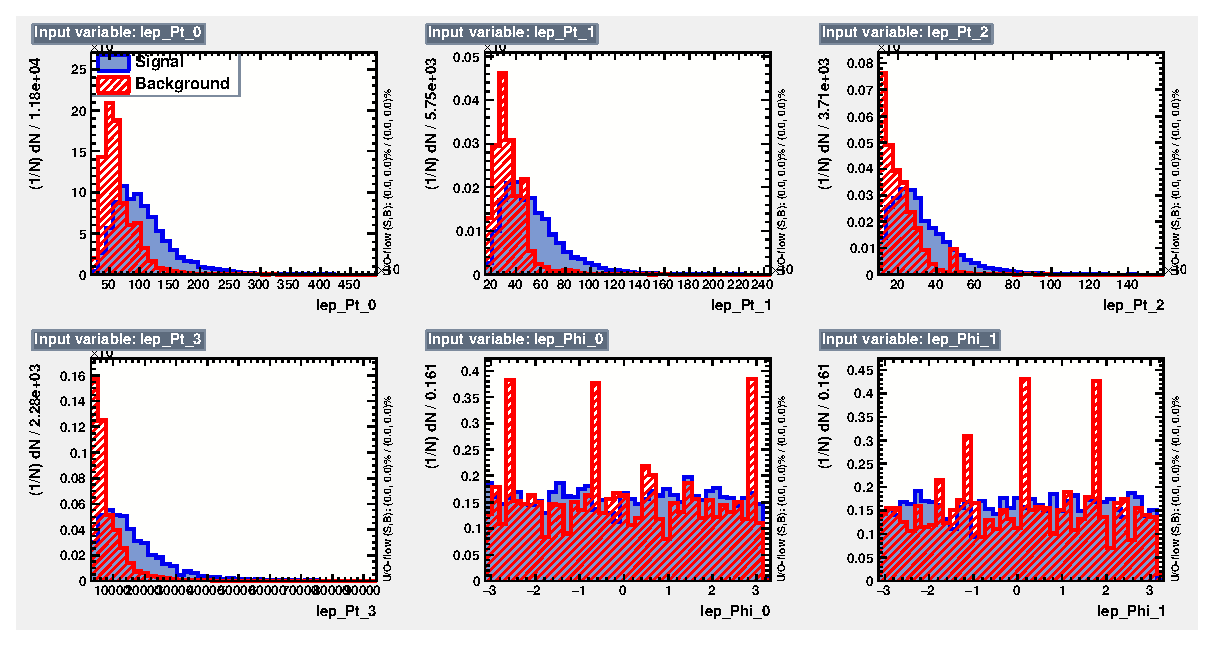
\includegraphics[width=0.4\textwidth]{figures/4lbb/variables_id_c1.eps}
	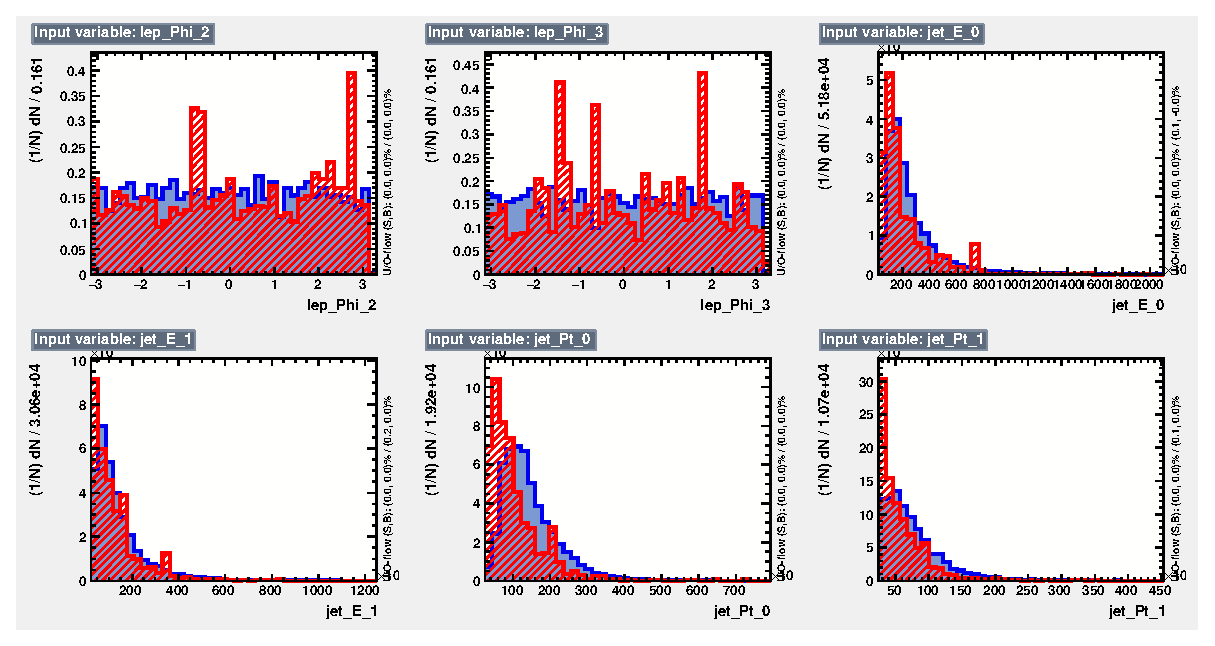
\includegraphics[width=0.4\textwidth]{figures/4lbb/variables_id_c2.eps}
	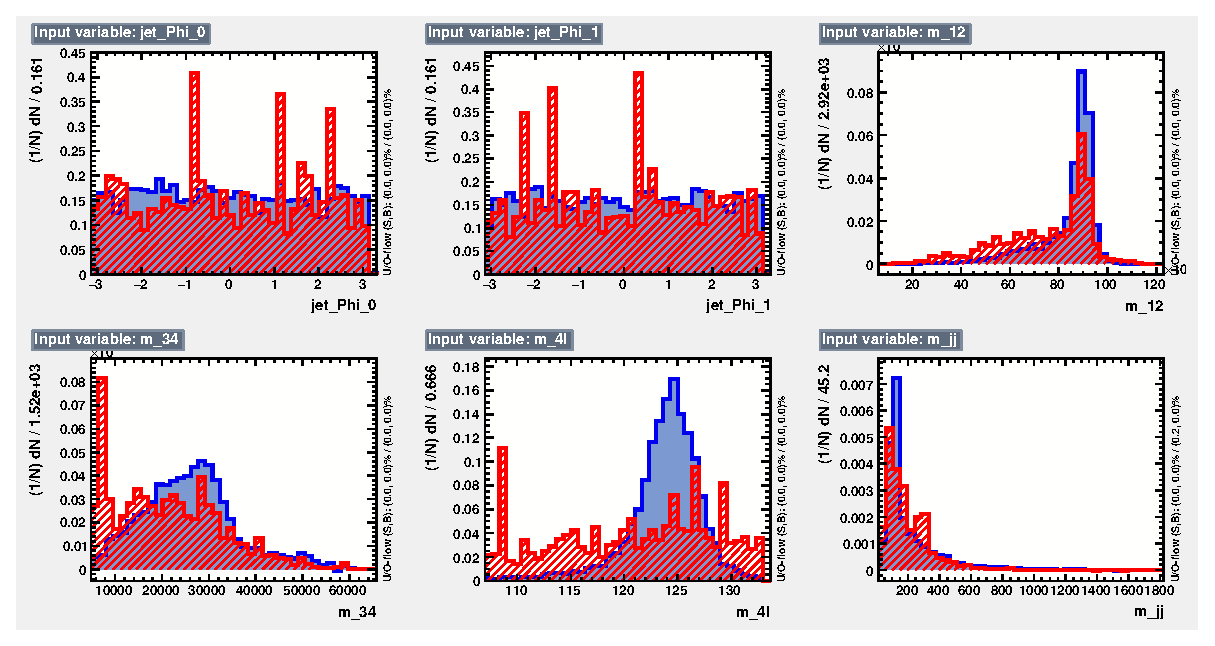
\includegraphics[width=0.4\textwidth]{figures/4lbb/variables_id_c3.eps}
	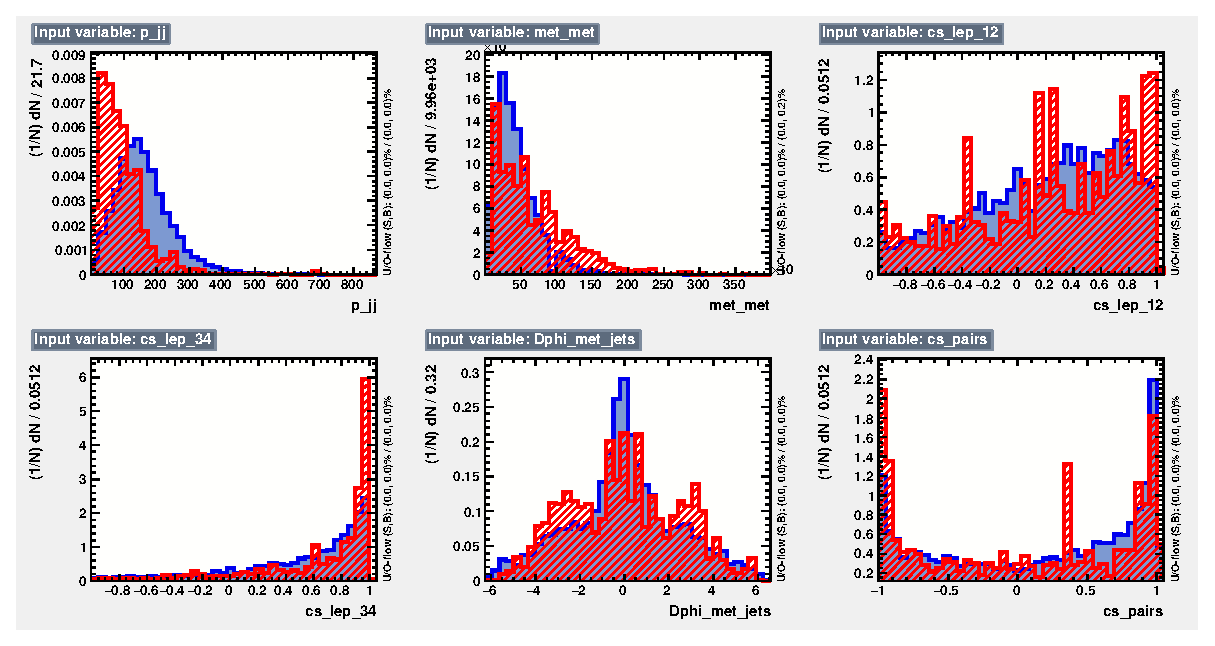
\includegraphics[width=0.4\textwidth]{figures/4lbb/variables_id_c4.eps}
	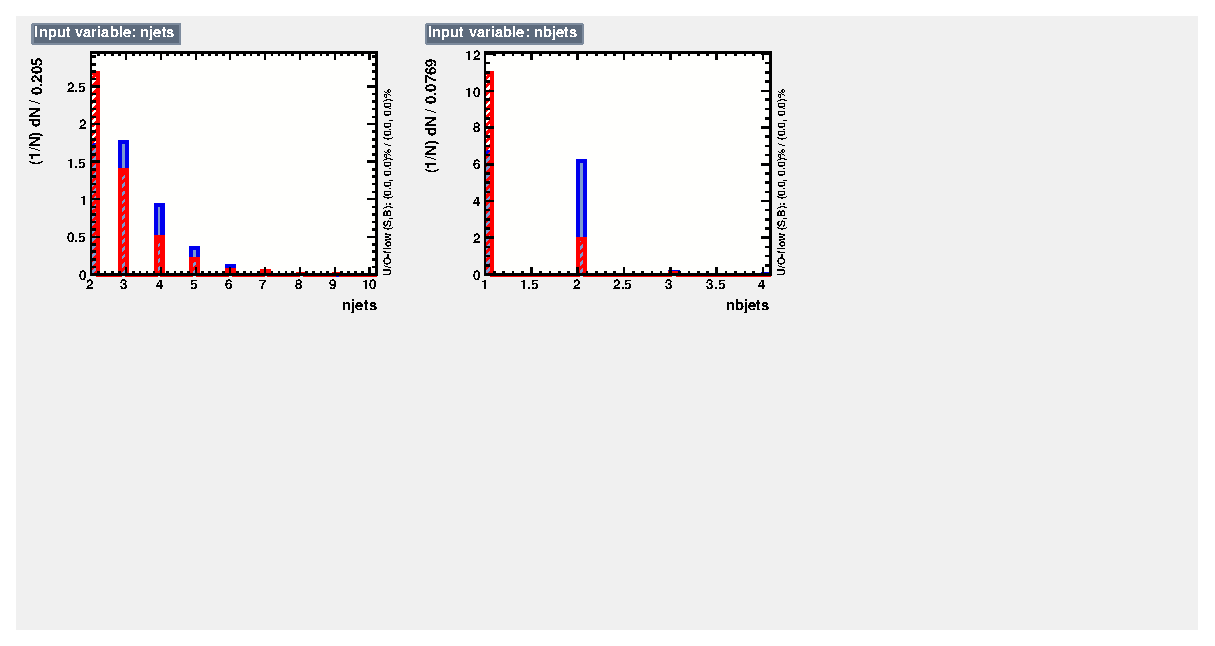
\includegraphics[width=0.4\textwidth]{figures/4lbb/variables_id_c5.eps}
\end{figure}

Events used for training is composed of randomly 90\% of the total events from the signal  and full backgrounds which pass the event selection. The rest of events are used for testing. The overtraining results is shown in Figure \ref{Fig.overtraining}. More details about the setup of the training can be found in Appendix \ref{app.bdt}

\begin{figure}[H]
	\caption{BDT overtraining results.}
	\label{Fig.overtraining}
	\centering
	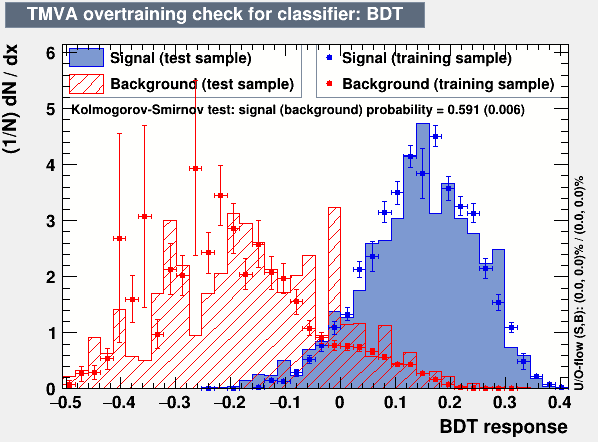
\includegraphics[width=0.6\textwidth]{figures/4lbb/overtrain_BDT.png}
\end{figure}

The classifier obtained from this training is applied on total signal and background samples and produces the outputs, i.e. BDT scores, of which the values vary between -0.6 to 0.4. The distribution of BDT score in SR is shown in Figure \ref{Fig.SR pre-fit}. 

\begin{figure}[H]
	\caption{BDT score distribution in SR. Dashed line represents signal normalized to total background}
	\label{Fig.SR pre-fit}
	\centering
	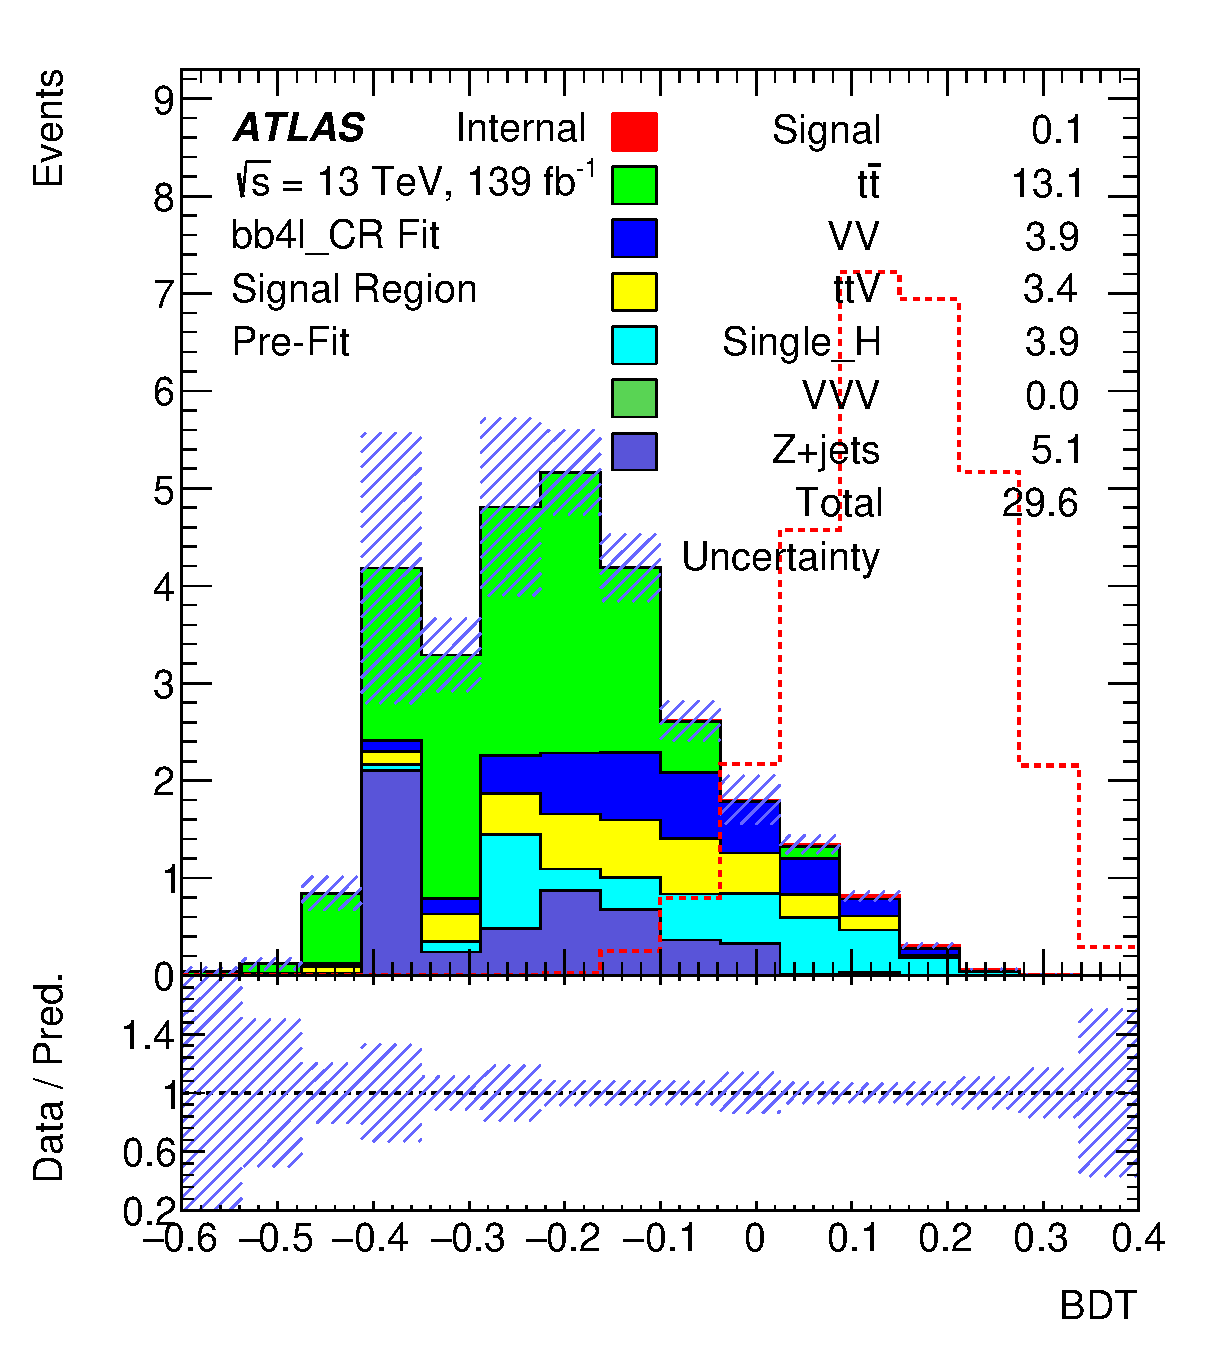
\includegraphics[width=0.6\textwidth]{figures/4lbb/Plots/SR.eps}
\end{figure}

\subsubsection{Background estimation}
\label{subsubsec:bkg}

As mentioned in Section \ref{sec:sample}, the dominant backgrounds in $4l+b\bar{b}$ channel include $t\bar{t}$, $t\bar{t}Z$, diboson, single Higgs and $Z$+jets processes. Since the signal selection uses some relatively loose cuts to improve the signal efficiency, processes with large cross section, like $t\bar{t}$, diboson and $Z$+jets, can have more events surviving from the selection and have the major contribution to the total backgrounds. Some other processes with exactly the same topology as the signal, like $t\bar{t}Z$ and Higgs production, also have some important contribution. To estimate these dominant backgrounds, several dedicated control regions (CRs) are defined to derive normalization corrections for the MC results in signal region (SR): $t\bar{t}$ CR for $t\bar{t}$, $t\bar{t}Z$ CR for $t\bar{t}Z$, $VV$+Higgs CR for the combination of diboson with single Higgs, and $Z$+jets CR for $Z$+jets. These normalization corrections have a uniform prior and are checked in a validation region (VR).

\paragraph{CR definitions}

In principle, the definitions of CRs should be as similar as possible with SR and satisfy that each CR is orthogonal to SR. This ensures that the normalization correction determined in the fit for the background results in an accurate estimate of the dominant backgrounds process in the signal regions. In this case, the following description will only mention about the differences between CRs with SR. The other definitions of CRs are kept the same with the event selection in SR which are mentioned in Section \ref{subsubsec:pre-selection}.

For the $t\bar{t}$ CR, the sub-leading lepton pair is required not to be $OSSF$ ($anti$-$OSSF$), which builds a phase space orthogonal to SR. The leading lepton pair should satisfy $M_{\rm leading\ pair}<$ 75 GeV or $M_{\rm leading\ pair}>$ 100 GeV to veto the $Z$ decay.

For the $t\bar{t}Z$ CR, the sub-leading lepton pair is required to be $anti$-$OSSF$. All the four leptons must pass the isolation with $PflowLoose$ working point to suppress $t\bar{t}$ process. The leading lepton pair should satisfy 85 GeV $<M_{\rm leading pair}<$ 100 GeV to suppress the processes without $Z$ decay. The requirement on the invariant mass of the quadruplet is removed to enhance $t\bar{t}Z$ process.

For the $VV$+Higgs CR, events are required to containing no $b$ jets by zero jets passing the $DL1r$ working point, which build a phase space orthogonal to SR. Also all the four leptons are required to pass the isolation.

For the $Z+$jets CR, the sub-leading pair is required to be $anti$-$OSSF$. The leading lepton pair should satisfy 85 GeV $<M_{\rm leading pair}<$ 100 GeV to suppress the processes without $Z$ decay. The missing transverse energy (MET) should satisfy $MET<$ 80 GeV to suppress $t\bar{t}$ process. The requirement on the number of $b$ jets is removed to enhanced $Z$+jets process.

Table \ref{Tab.CRs summary} gives a summary about all of the differences of these CRs compared with SR. The BDT classifier mentioned in Section \ref{subsubsec:mva} is applied to the data and MC results from all above CRs to obtain the BDT score distributions in each CR. The results are shown on Figure \ref{Fig.CRs pre-fit}.

\begin{table}[H]
\begin{center}
\caption{Control regions definition, only the differences with signal region listed.}
\label{Tab.CRs summary}
	\begin{tabular}{c|c}
		\toprule
		\toprule
		\multirow{2}{*}{$t\bar{t}$ CR}&$\ast$Sub-leading pair $anti$-$OSSF$\\
		&$\ast{M_{\rm leading\ pair}<75}$ GeV || $M_{\rm leading\ pair}>100$ GeV\\
		\midrule
		\multirow{4}{*}{$t\bar{t}V$ CR}&$\ast$Sub-leading pair $anti$-$OSSF$\\
		&$\ast$All four leptons pass the isolation\\
		&$\ast$85 GeV $<M_{\rm leading\ pair}<$ 100 GeV\\
		&$\ast$No requirement on $M_{\rm 4l}$\\
		\midrule
		\multirow{2}{*}{$VV$+Higgs CR}&$\ast{N_{\rm bjets}=0}$\\
		&$\ast$All four leptons pass the isolation\\
		\midrule
		\multirow{4}{*}{$Z$+jets CR}&$\ast$Sub-leading pair $anti$-$OSSF$\\
		&$\ast$85 GeV $<M_{\rm leading\ pair}<$ 100 GeV\\
		&$\ast{MET<80}$ GeV\\
		&$\ast$No requirement on $N_{\rm bjets}$\\
		\bottomrule
		\bottomrule
	\end{tabular}
\end{center}
\end{table}

\begin{figure}[H]
	\caption{Pre-fit results in each CR, the upper left one is $t\bar{t}$ CR, the upper right one is $t\bar{t}$V CR, the bottom left one is $VV$+Higgs CR, the bottom left one is $Z$+jets CR.}
	\label{Fig.CRs pre-fit}
	\centering
	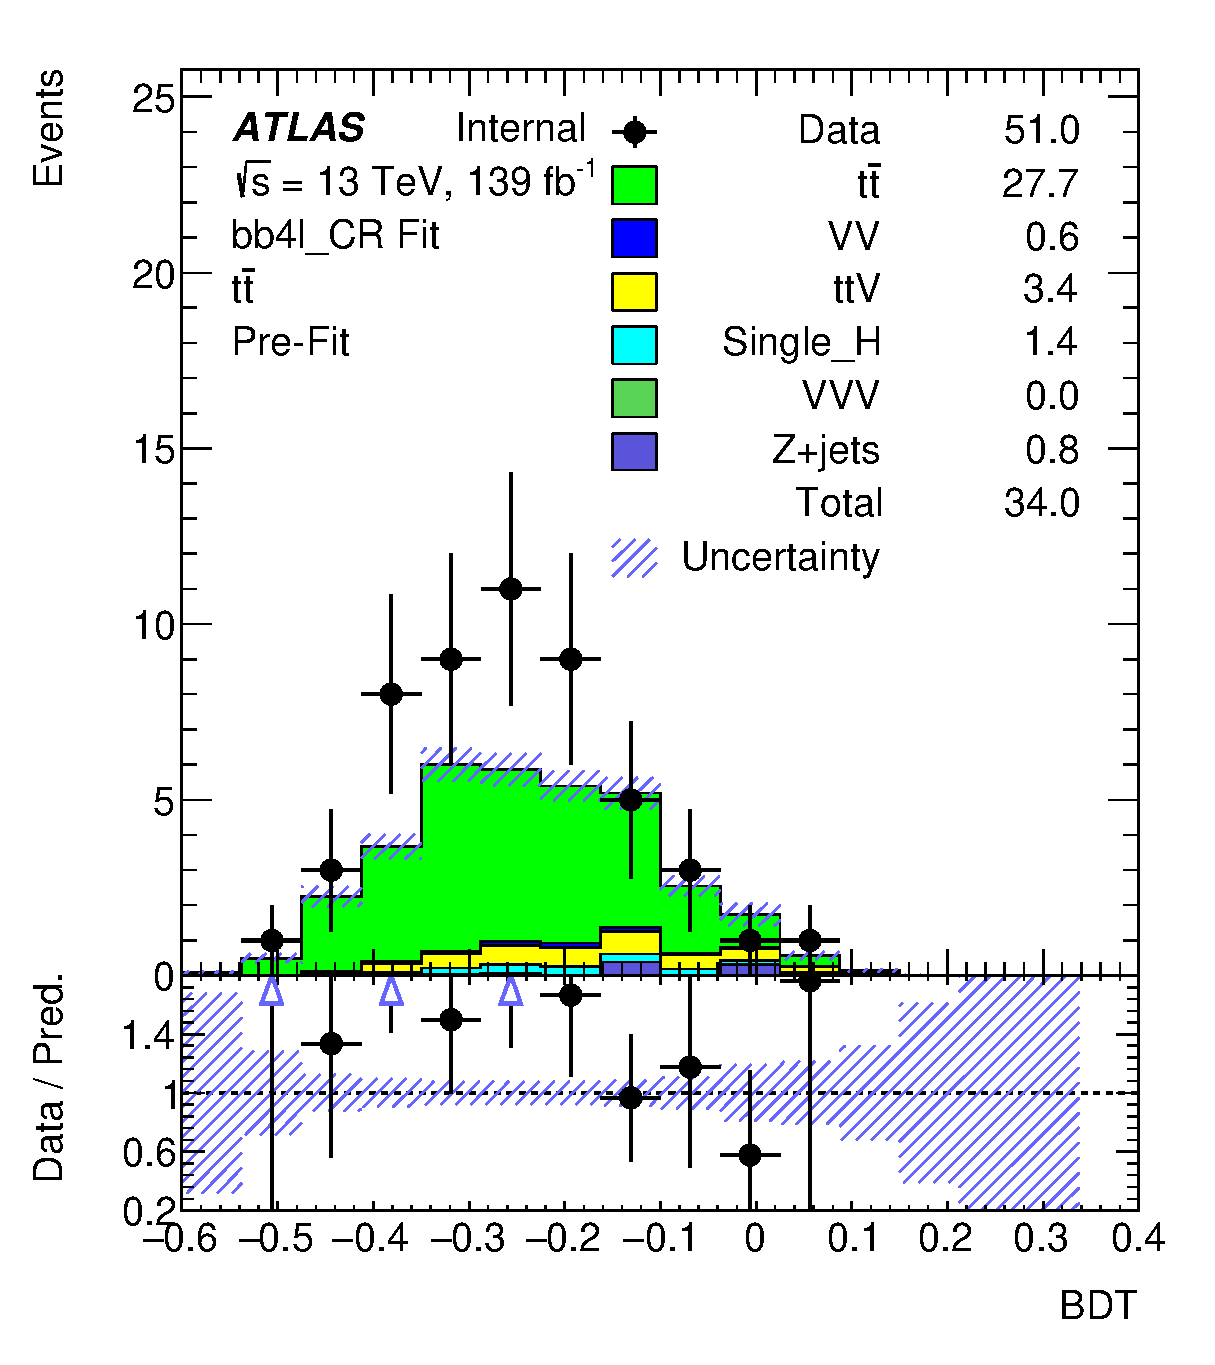
\includegraphics[width=0.4\textwidth]{figures/4lbb/Plots/tt_CR.eps}
	\includegraphics[width=0.4\textwidth]{figures/4lbb/Plots/ttV_CR.eps}
	\includegraphics[width=0.4\textwidth]{figures/4lbb/Plots/VVHiggsII_CR.eps}
	\includegraphics[width=0.4\textwidth]{figures/4lbb/Plots/Zjets_CR.eps}
\end{figure}

\paragraph{Fitting and validation}

The normalization corrections on MC results are derived from the background-only fits to data in the CRs. Distributions of BDT score are used to do this fitting as they contain the combined information from the observables listed in table, which can avoid strong correlation on some specific observables between CRs with SR or VR to ensure that the corrections can be extrapolated.

Table \ref{Tab.yields} compares the observed and predicted event yields, where the background event yields obtained after background-only fits in the corresponding control regions are also shown. The post-fit normalization correction factors for the dominant background processes, respectively $\mu_{t\bar{t}}=1.51\pm0.23,\mu_{t\bar{t}Z}=1.35\pm0.17,\mu_{VV}=0.77\pm0.39,\mu_{\rm Higgs}=1.12\pm0.37$, and $\mu_{Z+{\rm jets}}=0.5\pm0.18$, are also shown in Table \ref{Tab.yields}.

\begin{table}[H]
\begin{center}
\caption{Analysis region and background estimation summary, only statistical uncertainties included.}
\label{Tab.yields}
	\begin{tabular}{cccccc}
		\toprule
		\toprule
		\multicolumn{6}{c}{\textbf{Event Yields}}\\
		\midrule
		&$t\bar{t}$ CR&$t\bar{t}Z$ CR&$VV$+Higgs CR&$Z$+jets CR&VR\\
		\midrule
		Data	&51$\pm$7&82$\pm$9&43$\pm$7&40$\pm$6&303$\pm$17\\
		\midrule
		Total Bkg.&33.17$\pm$1.43&64.16$\pm$0.88&48.47$\pm$1.92&65.05$\pm$13.37&251.42$\pm$2.57\\
		\midrule
		$t\bar{t}$&31.53$\pm$1.18&2.23$\pm$0.31&0.96$\pm$0.21&3.54$\pm$0.40&61.15$\pm$1.56\\
		$t\bar{t}Z$&3.71$\pm$0.16&59.67$\pm$0.60&0.27$\pm$0.04&1.94$\pm$0.11&92.15$\pm$0.73\\
		$VV$	&0.60$\pm$0.06&4.05$\pm$0.16&21.77$\pm$0.28&6.13$\pm$0.23&79.05$\pm$0.51\\
		Higgs	&1.44$\pm$0.03&1.60$\pm$0.03&22.41$\pm$1.51&0.84$\pm$0.62&9.43$\pm$0.71\\
		$Z$+jets&0.05$\pm$0.79&2.85$\pm$0.54&3.09$\pm$1.14&51.89$\pm$13.33&9.15$\pm$1.69\\
		\midrule
		\midrule
		\multicolumn{6}{c}{\textbf{Post-fit Normalization}}\\
		\midrule
		\multicolumn{6}{c}{$\mu_{t\bar{t}}=1.51\pm0.23\mid\mu_{t\bar{t}Z}=1.35\pm0.17\mid\mu_{VV}=0.77\pm0.39\mid\mu_{\rm Higgs}=1.12\pm0.37\mid\mu_{Z+{\rm jets}}=0.5\pm0.18$}\\
		\bottomrule
		\bottomrule
	\end{tabular}
\end{center}
\end{table}

A VR enriched with events from the dominant backgrounds is built to check the normalization corrections. This VR only require the quadruplet satisfying $M_{\rm 4l}<$ 107 GeV or $M_{\rm 4l}>$ 133 GeV to be orthogonal to SR.

Distributions of BDT score in the control regions after performing background-only fits to data in the CRs and applying the dominant backgrounds normalization corrections are shown in Figure \ref{Fig.CRs post-fit}. In the VR, good agreement between the data and SM prediction provided by the post-fit MC simulation is observed for the BDT discriminant relevant to the analysis.

\begin{figure}[H]
	\caption{Post-fit results in each CR, the upper left one is $t\bar{t}$ CR, the upper right one is $t\bar{t}$V CR, the bottom left one is $VV$+Higgs CR, the bottom left one is $Z$+jets CR.}
	\label{Fig.CRs post-fit}
	\centering
	\includegraphics[width=0.4\textwidth]{figures/4lbb/Plots/tt_CR_postFit.eps}
	\includegraphics[width=0.4\textwidth]{figures/4lbb/Plots/ttV_CR_postFit.eps}
	\includegraphics[width=0.4\textwidth]{figures/4lbb/Plots/VVHiggsII_CR_postFit.eps}
	\includegraphics[width=0.4\textwidth]{figures/4lbb/Plots/Zjets_CR_postFit.eps}
\end{figure}

\begin{figure}[H]
	\caption{Pre-fit and post-fit results in VR, the left one is the pre-fit, the right one is the post-fit.}
	\label{Fig.VR}
	\centering
	\includegraphics[width=0.4\textwidth]{figures/4lbb/Plots/VR.eps}
	\includegraphics[width=0.4\textwidth]{figures/4lbb/Plots/VR_postFit.eps}
\end{figure}

\section{Systematic uncertainties}
\label{sec:error}

TBD

\section{Results}
\label{sec:results}

TBD

\section{Conclusions}
\label{sec:conclusion}

TBD



\clearpage
\section{The Analysis of 2L+$bb$+2j Channels }
\label{sec:LLbb2j}
Add the text for 2L$bb$2j channels



\clearpage
%\section{Signal region definition using multivariate analysis techniques}
\label{sec:eventselec}


%\clearpage
%\section{Fake lepton and tau background estimates}
\label{sec:nonpromptbkg}


%\clearpage
%\input{Tex/PromptBkgValidation.tex}
%\clearpage
%\section{Systematic uncertainties}
\label{sec:systematics}


%\clearpage
%\section{Signal regions before the fit}
\label{sec:signalregion}


%\clearpage
%\section{Results}
\label{sec:results}



%\clearpage
%\section{Conclusion}
\label{sec:conclusion}


%\clearpage

%Place your conclusion here.
% please each sub-channel analyst, please adds your sections in the following files
%\input{Tex/Chan2L.tex}
%\clearpage
%\input{Tex/3L.tex}
%\input{Tex/4L.tex}
%\section{The Analysis of $\gamma\gamma$+Lepton Channel }
\label{sec:AnaYYL}
Add the text for 3L



%\input{Tex/Taus.tex}
%\input{Tex/bb4L.tex}
%\input{Tex/2Lbb2j.tex}

%-------------------------------------------------------------------------------
% If you use biblatex and either biber or bibtex to process the bibliography
% just say \printbibliography here
\printbibliography
% If you want to use the traditional BibTeX you need to use the syntax below.
%\bibliographystyle{bib/bst/atlasBibStyleWithTitle}
%\bibliography{ANA-HDBS-2019-04-INT1,bib/ATLAS,bib/CMS,bib/ConfNotes,bib/PubNotes}
%-------------------------------------------------------------------------------

%-------------------------------------------------------------------------------
% Print the list of contributors to the analysis
% The argument gives the fraction of the text width used for the names
%-------------------------------------------------------------------------------
\clearpage
%The supporting notes for the analysis should also contain a list of contributors.
%This information should usually be included in \texttt{mydocument-metadata.tex}.
%The list should be printed either here or before the Table of Contents.
%\PrintAtlasContribute{0.30}


%-------------------------------------------------------------------------------
\clearpage
\appendix
\part*{Appendices}
\addcontentsline{toc}{part}{Appendices}
 %\input{Tex/AppAnaTwoLSS.tex}
% \clearpage
 %\section{Appendix of the Analysis of 3 Lepton Channel }
\label{sec:AppAnaThreeL}
Add Appendix of the text for 3L 



 %\clearpage
 %\input{Tex/AppAnaFourL.tex}
% \clearpage
 %\section{Appendix of the Analysis of $\gamma\gamma$+Lepton Channel }
\label{sec:AppAnaYYL}
Add appendix of the text for 3L



% \clearpage
 %\input{Tex/AppTaus.tex}
% \clearpage
 %\section{Appendix of the Analysis of $bb$ + 4l Channels }
\label{sec:Appbb4l}
Add Appendix of the text for $bb$+4l channels



 %\clearpage
 %\section{Appendix of the Analysis of 2L+$bb$+2j Channels }
\label{sec:AppLLbb2j}
Add appendix of the text for 2L$bb$2j channels



% \clearpage
 \section{Appendix of the  analysis of two Same Signed Lepton }
\label{sec:AppTwoLSS}
Add the Appendix of the text for 2LSS



 \clearpage
 \section{The Appendix of the Analysis of 3 Lepton Channel }
\label{sec:AppAnaThreeL}
Add the appendix of the text for 3L



 \clearpage
 \section{Appendix of the Analysis of 4 Lepton Channel }
\label{sec:AppAnaFourL}

\subsection{Analysis strategy}
\label{subsec:ana}

This analysis relies on the use of a multivariate discriminant designed to select candidate events consistent with non-resonant $HH$ production. To construct such a discriminant, a signal region is defined with some event selection criteria. Section \ref{subsubsec:pre-selection} describes these signal region selection criteria. Section \ref{subsubsec:mva} describes the architecture and the training of the Boosted Decision Tree (BDT) classifier from which the discriminant is constructed. Section \ref{subsubsec:bkg} describes the final background estimation procedure.

\subsubsection{Event selection}
\label{subsubsec:pre-selection}

To define the signal criteria, the analysis has some further requirements on each event. These events are triggered by any of the standard single electron and single muon, or di-leptons. Then trigger matching is applied to data and MC, requiring any of the selected leptons to be close to the corresponding trigger lepton within $\Delta{R}<0.1$.

In $4l+b\bar{b}$ channel, signal event are selected with exactly four leptons. The four leptons are sorted by $p_{T}$ number. Either of the third lepton and the forth lepton, with the third and forth highest $p_{T}$, is required to pass the $PflowLoose$ isolation working point. This loose selection can give a acceptable background rejection and good signal efficiency.

A angular separation of $\Delta{R}(l_{i},l_{j})=\sqrt{(\eta_{i}-\eta_{j})^{2}+(\phi_{i}-\phi_{j})^{2}}<0.1$ is required between any of lepton pairs.

In each quadruplet, the $p_{T}$ thresholds for the three leading leptons are 20,15 and 10 GeV.

The invariant mass of the $OSSF$ lepton pairs in each quadruplet is calculated. The lepton pair with invariant mass closest to the nominal $Z$ boson mass is selected as the leading lepton pair. The two remaining leptons are also required to be $OSSF$ and form the sub-leading lepton pair.

All the $OSSF$ lepton pairs are required to have invariant mass large than 5 GeV to veto the $J/\Psi$ decay.

Events are selected with at least two jets. The $DL1r$ algorithm is used to identify jets containing $b$-hadrons ($b$ jets). Events containing at least one $b$ jets are selected by requiring the number of jets passing a $DL1r$ working point, which gives a $b$-tagging efficiency of 77\%, no less than one.

Finally the invariant mass of the four leptons must satisfy 107 GeV$<M_{\rm 4l}<$ 133 GeV to select a on-shell Higgs decay. A comprehensive summary of all the cuts and requirements used in the event selection is shown in Table \ref{Tab.pre-selection}.

\begin{table}[H]
\begin{center}
\caption{The event selection used to define the signal criteria.}
\label{Tab.pre-selection}
\begin{tabular}{cc}
	\toprule
	\toprule	
	\multicolumn{2}{c}{\textbf{Event Selection}}\\
	\midrule
	\textbf{Trigger Matching}&Medium\\
	\midrule
	\textbf{Isolation}&\makecell[c]{Either of the third lepton and the forth lepton\\ passes the $PflowLoose$ isolation working point}\\
	\midrule
	\textbf{Separation}&$\Delta{R}(l_{i},l_{j})=\sqrt{(\eta_{i}-\eta_{j})^{2}+(\phi_{i}-\phi_{j})^{2}}<0.1$\\
	\midrule
	\textbf{Kinematics}&$p_{T}$ > 20, 15, 10 GeV for the three leading leptons\\
	\midrule
	\textbf{Pair Selection}&Two $OSSF$ lepton pairs\\
	\midrule
	\textbf{$J/\Psi$ veto}&All $OSSF$ lepton pairs have mass large than 5 GeV\\
	\midrule
	\textbf{Jets Number}&$N_{\rm jets}\ge{2}$\\
	\midrule
	\textbf{b Jets Number}&$N_{\rm b jets}\ge{1}$\\
	\midrule
	\textbf{Quadruplet Mass}&107 GeV $<M_{\rm 4l}<$ 133 GeV\\
	\bottomrule
	\bottomrule
\end{tabular}
\end{center}
\end{table}

\subsubsection{Multi-variable analysis}
\label{subsubsec:mva}

To enhance sensitivity to the signal process and to maximize rejection of the expected SM backgrounds, some observables from the selected events are checked and used for building a multivariate discriminant. The input variables are list in Table \ref{Tab.bdt inputs}. Distributions of these inputs are shown in Figure \ref{Fig.inputs}. This discriminant uses the outputs of a BDT classifier trained with the Toolkit for Multivariate Analysis (TMVA) which provides a ROOT-integrated environment for the processing.

\begin{table}[H]
\begin{center}
\caption{Variables used as inputs to the BDT classifier.}
\label{Tab.bdt inputs}
\begin{tabular}{cc}
	\toprule
	\toprule	
	Variables&Description\\
	\midrule
	$lep\_p_{T}\_*,lep\_\Phi\_*,$&$p_{T},\Phi$ of all the four leptons\\
	\midrule
	$jet\_p_{T}\_*,jet\_E\_*,jet\_\Phi\_*,$&$p_{T},E,\Phi$ of the two leading jets\\
	\midrule
	$M_{12},M_{34},M_{4l},M_{jj}$&\makecell[c]{Invariant mass of the leading lepton pair, \\sub-leading lepton pair, quadruplet and leading jets pair}\\
	\midrule
	$p_{T,4l},p_{T,jj}$&$p_{T}$ of the quadruplet and the leading jets pair\\
	\midrule
	MET&Missing transverse energy\\
	\midrule
	$cos\theta_{12},cos\theta_{34}$&\makecell[c]{Cosine of the angle between two leptons \\in the leading pair and sub-leading pair}\\
	\midrule
	$cos\theta_{pairs}$&Cosine of the angle between two lepton pairs\\
	\midrule
	$\Delta\Phi_{MET\&jets}$&$\Delta\Phi$ of the MET and leading jets\\
	\midrule
	$N_{jets},N_{bjets}$&The number of jets and b jets\\
	\bottomrule
	\bottomrule
\end{tabular}
\end{center}
\end{table}

\begin{figure}[H]
	\caption{Distributions of inputs for BDT training.}
	\label{Fig.inputs}
	\centering
	\includegraphics[width=0.4\textwidth]{figures/variables_id_c1.eps}
	\includegraphics[width=0.4\textwidth]{figures/variables_id_c2.eps}
	\includegraphics[width=0.4\textwidth]{figures/variables_id_c3.eps}
	\includegraphics[width=0.4\textwidth]{figures/variables_id_c4.eps}
	\includegraphics[width=0.4\textwidth]{figures/variables_id_c5.eps}
\end{figure}

Events used for training is composed of randomly 90\% of the total events from the signal  and full backgrounds which pass the event selection. The rest of events are used for testing. The overtraining results is shown in Figure \ref{Fig.overtraining}. More details about the setup of the training can be found in Appendix \ref{app.bdt}

\begin{figure}[H]
	\caption{BDT overtraining results.}
	\label{Fig.overtraining}
	\centering
	\includegraphics[width=0.6\textwidth]{figures/overtrain_BDT.png}
\end{figure}

The classifier obtained from this training is applied on total signal and background samples and produces the outputs, i.e. BDT scores, of which the values vary between -0.6 to 0.4. The distribution of BDT score in SR is shown in Figure \ref{Fig.SR pre-fit}. 

\begin{figure}[H]
	\caption{BDT score distribution in SR. Dashed line represents signal normalized to total background}
	\label{Fig.SR pre-fit}
	\centering
	\includegraphics[width=0.6\textwidth]{figures/Plots/SR.eps}
\end{figure}

\subsubsection{Background estimation}
\label{subsubsec:bkg}

As mentioned in Section \ref{sec:sample}, the dominant backgrounds in $4l+b\bar{b}$ channel include $t\bar{t}$, $t\bar{t}Z$, diboson, single Higgs and $Z$+jets processes. Since the signal selection uses some relatively loose cuts to improve the signal efficiency, processes with large cross section, like $t\bar{t}$, diboson and $Z$+jets, can have more events surviving from the selection and have the major contribution to the total backgrounds. Some other processes with exactly the same topology as the signal, like $t\bar{t}Z$ and Higgs production, also have some important contribution. To estimate these dominant backgrounds, several dedicated control regions (CRs) are defined to derive normalization corrections for the MC results in signal region (SR): $t\bar{t}$ CR for $t\bar{t}$, $t\bar{t}Z$ CR for $t\bar{t}Z$, $VV$+Higgs CR for the combination of diboson with single Higgs, and $Z$+jets CR for $Z$+jets. These normalization corrections have a uniform prior and are checked in a validation region (VR).

\paragraph{CR definitions}

In principle, the definitions of CRs should be as similar as possible with SR and satisfy that each CR is orthogonal to SR. This ensures that the normalization correction determined in the fit for the background results in an accurate estimate of the dominant backgrounds process in the signal regions. In this case, the following description will only mention about the differences between CRs with SR. The other definitions of CRs are kept the same with the event selection in SR which are mentioned in Section \ref{subsubsec:pre-selection}.

For the $t\bar{t}$ CR, the sub-leading lepton pair is required not to be $OSSF$ ($anti$-$OSSF$), which builds a phase space orthogonal to SR. The leading lepton pair should satisfy $M_{\rm leading\ pair}<$ 75 GeV or $M_{\rm leading\ pair}>$ 100 GeV to veto the $Z$ decay.

For the $t\bar{t}Z$ CR, the sub-leading lepton pair is required to be $anti$-$OSSF$. All the four leptons must pass the isolation with $PflowLoose$ working point to suppress $t\bar{t}$ process. The leading lepton pair should satisfy 85 GeV $<M_{\rm leading pair}<$ 100 GeV to suppress the processes without $Z$ decay. The requirement on the invariant mass of the quadruplet is removed to enhance $t\bar{t}Z$ process.

For the $VV$+Higgs CR, events are required to containing no $b$ jets by zero jets passing the $DL1r$ working point, which build a phase space orthogonal to SR. Also all the four leptons are required to pass the isolation.

For the $Z+$jets CR, the sub-leading pair is required to be $anti$-$OSSF$. The leading lepton pair should satisfy 85 GeV $<M_{\rm leading pair}<$ 100 GeV to suppress the processes without $Z$ decay. The missing transverse energy (MET) should satisfy $MET<$ 80 GeV to suppress $t\bar{t}$ process. The requirement on the number of $b$ jets is removed to enhanced $Z$+jets process.

Table \ref{Tab.CRs summary} gives a summary about all of the differences of these CRs compared with SR. The BDT classifier mentioned in Section \ref{subsubsec:mva} is applied to the data and MC results from all above CRs to obtain the BDT score distributions in each CR. The results are shown on Figure \ref{Fig.CRs pre-fit}.

\begin{table}[H]
\begin{center}
\caption{Control regions definition, only the differences with signal region listed.}
\label{Tab.CRs summary}
	\begin{tabular}{c|c}
		\toprule
		\toprule
		\multirow{2}{*}{$t\bar{t}$ CR}&$\ast$Sub-leading pair $anti$-$OSSF$\\
		&$\ast{M_{\rm leading\ pair}<75}$ GeV || $M_{\rm leading\ pair}>100$ GeV\\
		\midrule
		\multirow{4}{*}{$t\bar{t}V$ CR}&$\ast$Sub-leading pair $anti$-$OSSF$\\
		&$\ast$All four leptons pass the isolation\\
		&$\ast$85 GeV $<M_{\rm leading\ pair}<$ 100 GeV\\
		&$\ast$No requirement on $M_{\rm 4l}$\\
		\midrule
		\multirow{2}{*}{$VV$+Higgs CR}&$\ast{N_{\rm bjets}=0}$\\
		&$\ast$All four leptons pass the isolation\\
		\midrule
		\multirow{4}{*}{$Z$+jets CR}&$\ast$Sub-leading pair $anti$-$OSSF$\\
		&$\ast$85 GeV $<M_{\rm leading\ pair}<$ 100 GeV\\
		&$\ast{MET<80}$ GeV\\
		&$\ast$No requirement on $N_{\rm bjets}$\\
		\bottomrule
		\bottomrule
	\end{tabular}
\end{center}
\end{table}

\begin{figure}[H]
	\caption{Pre-fit results in each CR, the upper left one is $t\bar{t}$ CR, the upper right one is $t\bar{t}$V CR, the bottom left one is $VV$+Higgs CR, the bottom left one is $Z$+jets CR.}
	\label{Fig.CRs pre-fit}
	\centering
	\includegraphics[width=0.4\textwidth]{figures/Plots/tt_CR.eps}
	\includegraphics[width=0.4\textwidth]{figures/Plots/ttV_CR.eps}
	\includegraphics[width=0.4\textwidth]{figures/Plots/VVHiggsII_CR.eps}
	\includegraphics[width=0.4\textwidth]{figures/Plots/Zjets_CR.eps}
\end{figure}

\paragraph{Fitting and validation}

The normalization corrections on MC results are derived from the background-only fits to data in the CRs. Distributions of BDT score are used to do this fitting as they contain the combined information from the observables listed in table, which can avoid strong correlation on some specific observables between CRs with SR or VR to ensure that the corrections can be extrapolated.

Table \ref{Tab.yields} compares the observed and predicted event yields, where the background event yields obtained after background-only fits in the corresponding control regions are also shown. The post-fit normalization correction factors for the dominant background processes, respectively $\mu_{t\bar{t}}=1.51\pm0.23,\mu_{t\bar{t}Z}=1.35\pm0.17,\mu_{VV}=0.77\pm0.39,\mu_{\rm Higgs}=1.12\pm0.37$, and $\mu_{Z+{\rm jets}}=0.5\pm0.18$, are also shown in Table \ref{Tab.yields}.

\begin{table}[H]
\begin{center}
\caption{Analysis region and background estimation summary, only statistical uncertainties included.}
\label{Tab.yields}
	\begin{tabular}{cccccc}
		\toprule
		\toprule
		\multicolumn{6}{c}{\textbf{Event Yields}}\\
		\midrule
		&$t\bar{t}$ CR&$t\bar{t}Z$ CR&$VV$+Higgs CR&$Z$+jets CR&VR\\
		\midrule
		Data	&51$\pm$7&82$\pm$9&43$\pm$7&40$\pm$6&303$\pm$17\\
		\midrule
		Total Bkg.&33.17$\pm$1.43&64.16$\pm$0.88&48.47$\pm$1.92&65.05$\pm$13.37&251.42$\pm$2.57\\
		\midrule
		$t\bar{t}$&31.53$\pm$1.18&2.23$\pm$0.31&0.96$\pm$0.21&3.54$\pm$0.40&61.15$\pm$1.56\\
		$t\bar{t}Z$&3.71$\pm$0.16&59.67$\pm$0.60&0.27$\pm$0.04&1.94$\pm$0.11&92.15$\pm$0.73\\
		$VV$	&0.60$\pm$0.06&4.05$\pm$0.16&21.77$\pm$0.28&6.13$\pm$0.23&79.05$\pm$0.51\\
		Higgs	&1.44$\pm$0.03&1.60$\pm$0.03&22.41$\pm$1.51&0.84$\pm$0.62&9.43$\pm$0.71\\
		$Z$+jets&0.05$\pm$0.79&2.85$\pm$0.54&3.09$\pm$1.14&51.89$\pm$13.33&9.15$\pm$1.69\\
		\midrule
		\midrule
		\multicolumn{6}{c}{\textbf{Post-fit Normalization}}\\
		\midrule
		\multicolumn{6}{c}{$\mu_{t\bar{t}}=1.51\pm0.23\mid\mu_{t\bar{t}Z}=1.35\pm0.17\mid\mu_{VV}=0.77\pm0.39\mid\mu_{\rm Higgs}=1.12\pm0.37\mid\mu_{Z+{\rm jets}}=0.5\pm0.18$}\\
		\bottomrule
		\bottomrule
	\end{tabular}
\end{center}
\end{table}

A VR enriched with events from the dominant backgrounds is built to check the normalization corrections. This VR only require the quadruplet satisfying $M_{\rm 4l}<$ 107 GeV or $M_{\rm 4l}>$ 133 GeV to be orthogonal to SR.

Distributions of BDT score in the control regions after performing background-only fits to data in the CRs and applying the dominant backgrounds normalization corrections are shown in Figure \ref{Fig.CRs post-fit}. In the VR, good agreement between the data and SM prediction provided by the post-fit MC simulation is observed for the BDT discriminant relevant to the analysis.

\begin{figure}[H]
	\caption{Post-fit results in each CR, the upper left one is $t\bar{t}$ CR, the upper right one is $t\bar{t}$V CR, the bottom left one is $VV$+Higgs CR, the bottom left one is $Z$+jets CR.}
	\label{Fig.CRs post-fit}
	\centering
	\includegraphics[width=0.4\textwidth]{figures/Plots/tt_CR_postFit.eps}
	\includegraphics[width=0.4\textwidth]{figures/Plots/ttV_CR_postFit.eps}
	\includegraphics[width=0.4\textwidth]{figures/Plots/VVHiggsII_CR_postFit.eps}
	\includegraphics[width=0.4\textwidth]{figures/Plots/Zjets_CR_postFit.eps}
\end{figure}

\begin{figure}[H]
	\caption{Pre-fit and post-fit results in VR, the left one is the pre-fit, the right one is the post-fit.}
	\label{Fig.VR}
	\centering
	\includegraphics[width=0.4\textwidth]{figures/Plots/VR.eps}
	\includegraphics[width=0.4\textwidth]{figures/Plots/VR_postFit.eps}
\end{figure}

\section{Systematic uncertainties}
\label{sec:error}

TBD

\section{Results}
\label{sec:results}

TBD

\section{Conclusions}
\label{sec:conclusion}

TBD

 \clearpage
 \section{Appendix of the Analysis of $\gamma\gamma$+Lepton Channel }
\label{sec:AppAnaYYL}
Add appendix of the text for 3L



 \clearpage
 \section{Appendix of the Analysis of $\tau$ Channels }
\label{sec:Apptaus}
Add the Appendix of the text for $\tau$ channels



 \clearpage
 \section{Appendix of the Analysis of $bb$ + 4l Channels }
\label{sec:Appbb4l}
Add Appendix of the text for $bb$+4l channels



 \clearpage
 \section{Appendix of the Analysis of 2L+$bb$+2j Channels }
\label{sec:AppLLbb2j}
Add appendix of the text for 2L$bb$2j channels



%-------------------------------------------------------------------------------

In an ATLAS note, use the appendices to include all the technical details of your work
that are relevant for the ATLAS Collaboration only (e.g.\ dataset details, software release used).
This information should be printed after the Bibliography.

\end{document}
